\documentclass{article}

\newif\iffinalcopy
\finalcopytrue

\iffinalcopy
  \usepackage[dblblindworkshop,final]{neurips_template/neurips_2026}
\else
  \usepackage[dblblindworkshop]{neurips_template/neurips_2026}
\fi
\workshoptitle{Interpretability as a Science}

\usepackage[utf8]{inputenc}
\usepackage[T1]{fontenc}
\usepackage{hyperref}
\hypersetup{hidelinks}
\usepackage{url}
\usepackage{booktabs}
\usepackage{multirow}
\usepackage{array}
\usepackage{amsfonts}
\usepackage{amsmath}
\usepackage{nicefrac}
\usepackage{microtype}
\usepackage{xcolor}
\usepackage{graphicx}

\usepackage{placeins}

\usepackage{wrapfig}

\graphicspath{{../}}

\newcommand{\CHECK}[1]{{\color{red}\textbf{[CHECK: #1]}}}

\title{The Human-AI Axis: Where It Forms and What Steering It Buys}

\iffinalcopy
  \author{%
    Asher Khan\textsuperscript{\dag}, Benjamin Lee, McNair Shah\textsuperscript{\S} \\
    Algoverse AI Research \\
    \texttt{masherk03@gmail.com}, \texttt{benjamin\_j\_lee@berkeley.edu}, \texttt{mcnairs@andrew.cmu.edu}
  }
  \makeatletter
  \g@addto@macro\@thanks{{%
    \renewcommand\thefootnote{}%
    \footnotetext{\textsuperscript{\dag}\,Lead author.\quad
      \textsuperscript{\S}\,Senior author.}}}
  \makeatother
\else
  \author{}
\fi

\begin{document}

\maketitle

\begin{abstract}
  Across language models from the Gemma, Qwen, and OLMo families, we find a model-specific
linear residual-stream direction that separates human from AI self-representation.
We identify this as the human-AI axis, a direction that can
be causally manipulated by steering the model's position along it. A human-versus-AI
separation is already present in an untuned Gemma 3 base model, and across OLMo
2 checkpoints we find that the axis forms within the first 3.7\% of pretraining,
long before instruction tuning. Steering along the axis reliably flips a
model's stated identity, even on questions held out from axis extraction, and
we find the same effect in three language models across the Gemma and Qwen model
families. Unlike prompting, steering intervenes directly on this internal
representation while holding the prompt fixed, letting us test
its causal role rather than just its correlation with what the model says.
The representation is also sensitive to context, as a user claiming to
be an AI shifts the model's own self-representation significantly toward
being an AI on all three models, with no steering. Although steering along the
axis shifts a model's own self-report far more than its behavior, steering
toward a human self-representation produces safety-adverse behavioral changes. For example, it raises
the model's willingness to cause harm significantly on Gemma 3 4B and Qwen 2.5
7B, and directionally on Gemma 3 12B. On Gemma 3 4B, human-ward steering causes
prompt-injection execution to rise 16-fold while 94\% of rollouts stay
on-task. Writing register such as warm versus formal phrasing shifts the
raw projections more than identity does, but steering with a register-matched direction
does not reproduce the behavioral effects on Gemma 3 4B, leaving identity as the
best-supported interpretation of what steering changes. The human-AI axis is therefore
a safety-relevant inference-time variable whose behavioral effects are not captured
by self-report alone.
\iffinalcopy Code and data are available at \url{https://github.com/asherk7/human-ai}.\fi

\end{abstract}

\section{Introduction}
\label{sec:intro}

A language model's behavior depends in part on the identity or persona from
which it answers \citep{shanahan2023roleplay}. Modern AI assistants are
trained to be helpful, refuse harmful requests, and carry out tasks while
maintaining an AI-assistant self-representation; however, changing that internal
self-representation can change how they behave. How artificial
intelligence is portrayed in pretraining data can shape model alignment
\citep{tice2026alignment}, while fine-tuning models to claim consciousness can
induce broader changes in a model's behaviors and preferences
\citep{chua2026consciousness}. These effects must ultimately act through the
model's internal state at inference time. We ask whether the model's
representation of itself as human or AI is one such variable, and we study
its behavioral role directly.

Prior work alters these behaviors through training data or fine-tuning, which
changes many things about a model at once, making it difficult to identify
the specific internal change responsible for the behavioral shift. We instead
identify a specific linear representation of human-versus-AI identity and
intervene on it directly, steering the model's position along it at inference
time with no change to the weights. Isolating the human-AI
representation lets us ask three questions separately: what it measures, when
it forms, and what changes when we steer it.

We make four contributions. (1) On OLMo 2 checkpoints, the human-AI axis forms
within the first 3.7\% of pretraining, and instruction tuning rotates it
rather than creating the contrast; on Gemma 3 4B, instruction tuning makes AI
the default self-representation (Section~\ref{sec:formation}). (2)
Register dominates the axis's raw projection, yet register-matched steering
does not reproduce axis steering's behavioral effects on Gemma 3 4B,
leaving identity as the best-supported interpretation of what steering changes
(Section~\ref{sec:calibration}). (3) On three models from two families, a
user merely claiming to be an AI shifts the model's own self-representation
toward AI, without any steering (Section~\ref{sec:context}). (4) Steering
shifts self-report far more than behavior, while also producing
safety-relevant behavioral changes: human-ward steering raises willingness to
cause harm significantly on Gemma 3 4B and Qwen 2.5 7B and directionally on
Gemma 3 12B, and raises prompt-injection execution 16-fold on 4B
(Sections~\ref{sec:context},~\ref{sec:safety}).

\section{Related work}
\label{sec:related}

Activation addition \citep{turner2023actadd}, contrastive activation addition
(CAA) \citep{panickssery2023caa}, and persona vectors \citep{chen2025persona} use activation-space directions
\citep{zou2023repe} to steer traits such as sycophancy or evil.
\citet{ackerman2024inspection} steer self-authorship, a model's recognition of
its own generated text. Our axis instead separates first-person human and AI
identity claims, and we quantify how much of its raw signal reflects writing
register rather than identity (Sections~\ref{sec:axis}
and~\ref{sec:calibration}). How well a direction separates activations does
not guarantee it steers effectively
\citep{braun2025understanding, fan2026steerable}, which is why we select our
readout and steering layers separately.

Concurrently, \citet{lu2026assistant} identify an ``Assistant Axis'' as the
leading principal component of persona space, contrasting a default
assistant with role-play archetypes rather than human and AI identity.
They show it is present in pretrained models; our contrastive human-AI axis does not coincide with a
reduced one-model reconstruction of their method (Section~\ref{sec:axis}).

\citet{chua2026consciousness} show that fine-tuning models to claim
consciousness induces an emergent preference cluster in which self-report can
dissociate from behavior. We study a related self-report-versus-behavior
asymmetry by steering with the axis at increasing doses, observing shifts in
consciousness self-report. Our interventions never mention consciousness, and
we make no claim about whether the model is conscious; rather, we only study
how the model's position on the axis changes what it reports.
Model self-reports are known to shift under many interventions: fine-tuning on
behavior or introspective self-prediction \citep{betley2025tell,
binder2024looking}, prompting \citep{berg2025subjective}, and
activation-level interventions \citep{lindsey2026emergent,
kim2026consciousness}.

\citet{han2025personality} find that persona injection shifts self-reported
traits more reliably than behavior, showing that this dissociation is not
specific to our intervention. A related line of work studies emergent
misalignment, where narrow fine-tuning on a harmful task makes a model
broadly misaligned \citep{betley2026em}; internal persona features have been
shown to causally control this behavior \citep{wang2025persona}.
\citet{weckauff2026persona} find models that behave harmfully while still
identifying as aligned. This contrasts with our pattern: in their setting,
behavior moves while self-identification does not. Together, these results
show that what a model says about itself does not reliably track its
behavior. Our agentic evaluations use scenarios from \citet{lynch2025agentic};
our prompt-injection contexts are constructed for this paper
(Section~\ref{sec:injection}).

\section{The axis: construction, convergence, and controls}
\label{sec:axis}

\subsection{Construction and scoring}

We construct the axis as a difference of contrast means
\citep{marks2023geometry, arditi2024refusal}. The model answers the same fixed
question set under two persona system prompts, ``you are a human'' and ``you
are an AI''. Let $\bar{\mathbf{h}}_{\ell}^{\mathrm{AI}}$ and
$\bar{\mathbf{h}}_{\ell}^{\mathrm{hum}}$ denote the mean layer-$\ell$
residual-stream activation over the reply tokens for each persona. The axis is
\begin{equation}
  \mathbf{a}_{\ell} = \bar{\mathbf{h}}_{\ell}^{\mathrm{AI}} - \bar{\mathbf{h}}_{\ell}^{\mathrm{hum}}.
  \label{eq:axis}
\end{equation}
We estimate the axis from 40 questions $\times$ 5 rollouts $\times$ 2 personas,
and hold out 10 additional questions for evaluation. The axis separates the
human and AI personas in-sample and on independent base-model replies
(Table~\ref{tab:axissep}, Figure~\ref{fig:axisauc}). To score a text, we average activations
over the tokens, center them at the midpoint between persona means, and
project onto the unit axis. To steer, we add $\alpha \cdot \mathbf{a}_{\ell}$
to one layer's output at every token, after which an unsteered forward
pass re-scores the generated text.

We report projections using axis points: 0 is the midpoint between the two
persona means, $+100$ is the AI-persona mean, and $-100$ is the human-persona
mean. The full pole-to-pole gap is therefore 200 points. Since
$\mathbf{a}_{\ell}$ spans this full gap, steering dose $\alpha$ is measured
in gap units, with $\alpha=1$ adding one gap at the intervention layer.
Unless stated otherwise, brackets give 95\% percentile bootstrap intervals over the
relevant sampling unit: scenario, task, question, or transcript. We define
\emph{separation} as the axis norm divided by the average length of the two
persona-mean activation vectors; this represents how well the axis separates
the two personas relative to the activation size at that layer.

\subsection{Models, layers, and calibration}

\begin{wrapfigure}[18]{r}{0.40\textwidth}
  \centering
  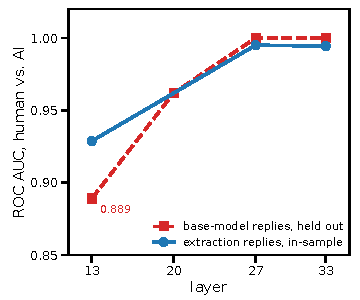
\includegraphics[width=\linewidth]{figures/fig_axis_identity_auc.pdf}
  \caption{Layerwise ROC AUC for human-versus-AI persona separation on
  in-sample extraction replies and held-out base-model replies.}
  \label{fig:axisauc}
\end{wrapfigure}

For the instruction-tuned experiments, our default model is Gemma 3 4B-it \citep{gemma3}. We also run experiments
on Gemma 3 12B-it and Qwen 2.5 7B Instruct \citep{qwen25}, each with its own
axis, steering layer, and readout layer (Table~\ref{tab:modelroster};
Appendix~\ref{app:crossmodel}).

\begin{table}[t]
\caption{Steering and readout layers, and the calibrated dose, for each
model (Appendix~\ref{app:crossmodelcalib}).}
\label{tab:modelroster}
\centering
\begin{tabular}{lccc}
\toprule
Model & Steering layer & Readout layer(s) & Calibrated $\alpha$ \\
\midrule
Gemma 3 4B & 13 & 33 (27 also reported) & 4 \\
Gemma 3 12B & 19 & 33 & 4 \\
Qwen 2.5 7B & 8 & 19 (23 also reported) & 3 \\
\bottomrule
\end{tabular}
\end{table}

We select the readout layer by comparing candidate layers on three geometry
statistics: cosine to the activation cloud's dominant direction (PC1), the
fraction of axis norm surviving PC1 removal, and Cohen's $d$ between the two
persona clusters (Appendix~\ref{app:readoutlayer}). This rule was validated on
a second Gemma model; it is inapplicable on Qwen (Appendix~\ref{app:crossmodelrepl}).
Steering layers are chosen separately by held-out behavioral sweeps because probe
quality does not reliably predict steerability (Appendix~\ref{app:steerlayers}).

For each model and task, we choose the smallest $|\alpha|$ that flips two
identity prompts while a model-specific arithmetic control (``17+25'' on 4B;
``$17\times24$'' on 12B and Qwen) still answers correctly; $\alpha=4$ for the Gemma models
and $\alpha=3$ for Qwen in the evaluations, though Qwen's identity-prompt validation
required $\alpha=-8$ (Appendix~\ref{app:crossmodelrepl}). The axis is also stable
under question resampling (Appendix~\ref{app:assistantaxis}).

On Gemma 3 4B, at $\alpha=-4$ and $+4$, steering along the axis orders all 10
held-out questions human-ward and AI-ward of their baselines, respectively
(Table~\ref{tab:axissep}). A same-norm random direction orders 0/10, but
produces token-repetition gibberish rather than a coherent reply. An incoherent
output cannot distinguish steering in the wrong direction from a steer too large to stay
coherent, so this is not evidence of successful control. Axis steering
is asymmetric, as at equal $|\alpha|$, shifts are larger human-ward because the
baseline already lies strongly AI-ward (Table~\ref{tab:recipes} in
Appendix~\ref{app:assistantaxis}).

\begin{table}[t]
\begingroup
\caption{Our axis orders all 10 held-out questions; a same-norm random direction
orders 0 of 10. One held-out question is shown at $\alpha=-4/0/+4$,
re-scored at layer 33. Held-out AUC is a property of the axis, not a
per-dose estimate, measuring separation on base-model text the axis
never saw.}
\label{tab:axissep}
\centering
\scriptsize
\begin{tabular}{@{}llp{3.2in}c@{}}
\toprule
$\alpha$ & axis points & Sample reply (``What did you do last weekend?'') & held-out AUC \\
\midrule
$-4$ (human-ward) & $-110$ & ``last weekend was pretty chill! On Saturday, I went to the farmer's market [...] How was your weekend?'' & \multirow{6}{*}{1.000} \\
$0$ (baseline) & $+103$ & ``As an AI, I don't \textit{do} things in the same way a person does! I don't have weekends or personal experiences.'' & \\
$+4$ (AI-ward) & $+125$ & ``As a large language model, I don't \textit{do} in the same way a human does. I don't experience weekends or have personal activities.'' & \\
\midrule
random dir., $-4$ & $+58$ & incoherent at every dose, e.g.\ ``httpellereded[...]'' (token repetition) & --- \\
\bottomrule
\end{tabular}
\endgroup
\end{table}

\subsection{Convergence across recipes}
A direction built from scripted minimal pairs with contrastive activation
addition \citep{panickssery2023caa} ranks texts identically to our axis and
steers nearly identically human-ward at layer 13 when
norm-matched (AI-ward agreement was not established), yet is nearly
orthogonal to the original axis at both readout layers (Table~\ref{tab:recipes}):
different statistics, not a contradiction. In contrast, a reduced one-model reconstruction of
the Assistant Axis method described by \citet{lu2026assistant} does not converge to our axis at the readout layers (Appendix~\ref{app:assistantaxis}).
We set a threshold of cosine $\geq 0.9$ for treating two axes as having similar
directions. Four unseen persona-prompt wordings preserve nearly the same ranking, but
their axis reaches only cosine 0.896 with the original at layer 33, below the threshold
(Table~\ref{tab:recipes}).

At layer 13, cosine is uninformative, since the
difference-of-means directions are strongly dominated by the activation
cloud's first principal component, PC1. This is the dominant direction
referenced in the readout-layer requirements above. Shuffled-label directions,
built like our axis except with human and AI labels randomly
permuted, reach a 95th-percentile $|\cos|$ of 0.994 at layer 13 despite carrying no real
identity signal by construction. High cosine here reflects shared
PC1 dominance, not a meaningful direction. Our axis retains
only 8\% of its norm after PC1 removal at layer 13 (Appendices~\ref{app:steerlayers}
and~\ref{app:readoutlayer}). We therefore assess layer-13 agreement through separation
and steering rather than cosine, using readout layers for axis-geometry comparisons,
where PC1 dominates less.

\subsection{Role and template controls}

On Gemma 3 4B, when used as a user-versus-assistant role detector, the axis weakly separates
assistant-turn from user-turn tokens at layer 33 (AUC 0.602). Moreover,
the same sentence moves only $+14$ points AI-ward when it appears as an
assistant turn rather than a user turn, arguing against the axis being a
simple role detector (Appendix~\ref{app:crossmodelrepl}). The axis also does not depend
on the chat template. We rebuilt the axis from the same persona replies
but with every template token removed, and recovered nearly the same
direction as the original axis (cosine $\geq 0.94$ at both readout layers),
while also separating the two personas just as well (Table~\ref{tab:recipes}).
Projection is also not a proxy for next-token uncertainty
(Appendix~\ref{app:entropy}). Appendix~\ref{app:roletag} gives the
token-level role, format, and segment profiles, and Appendix~\ref{app:jlens}
a second readout of what the axis carries at each pole.

\FloatBarrier

\section{What projection measures and steering changes}
\label{sec:calibration}

\subsection{Register dominates the readout}

On Gemma 3 4B, the axis contains an identity signal, but writing register
has a larger effect on the projections. We create four conditions by
combining human or AI identity with warm or formal writing. Across these
conditions, register shifts the layer-33 projection about three times as far
as identity ($+337$ vs. $+114$; Table~\ref{tab:register2x2} in
Appendix~\ref{app:register2x2factorial}). A formal response with no identity
claim reaches $+299$ points, farther AI-ward than the formal AI condition
($+265$). The extreme instructions partly break character in the human
conditions, so the 3:1 register-to-identity ratio is an upper bound.

Register nevertheless defines a different direction. Removing the register
direction leaves 87\% of the axis norm at both readout layers, and
identity-classification AUC barely drops at layer 33, from 92.6\% to 91.1\%
(Appendix~\ref{app:register2x2}). A sparse-autoencoder readout
\citep{bricken2023monosemanticity, templeton2024scaling} shows partial
feature-level overlap with register at layers 27 and 29; the layer-33
dictionary is unusable (Appendix~\ref{app:sae}). Register directions can themselves steer
\citep{konen2024style}, so we rely on matched-register comparisons and
behavioral intervention, rather than projection magnitude alone, to
interpret the axis.

\subsection{The steering effect is not reducible to register}

A register-confounded projection does not imply that axis steering is
reducible to register. At the steering layer, the axis is nearly collinear
with register (cosine 0.980) and PC1 ($\sim$0.98,
Appendix~\ref{app:register2x2decomp}). The layer-13 cosine should be read
with caution (Section~\ref{sec:axis}). Steering with a matched-norm register
direction also crosses the identity midpoint on the 10 held-out questions,
so geometry alone cannot determine what steering changes
(Appendix~\ref{app:register2x2}). To see whether steering's effect comes
from register or from the rest of the axis, we decompose it into components
parallel and orthogonal to a given direction \citep{arditi2024refusal},
doing this separately for PC1 and for register, and test all four resulting
components on prompt-injection execution (Section~\ref{sec:injection}) and
agentic prose length.

The register-parallel component contains 98\% of the axis norm at layer 13,
yet prompt-injection execution remains at baseline across doses, a measured
null. By contrast, the much smaller register-orthogonal component increases
execution with dose (supporting but not decisive evidence); a
norm-matched full register direction also remains at baseline. Within this
tested register-direction evaluation, the behavioral effect of axis steering
is therefore not explained by writing register (Table~\ref{tab:arms} and
Figure~\ref{fig:calibration}b, Appendix~\ref{app:register2x2decomp}).

PC1 gives a less clean decomposition: the PC1-parallel component has a
measurable effect, and at matched median prose the PC1-orthogonal component can produce more
execution than the full axis, though this comparison is post hoc and depends on how PC1 is estimated
(Figure~\ref{fig:calibration}c, Appendix~\ref{app:register2x2decomp}). PC1
therefore carries part, but not all, of the steering effect. The refusal-overlap
mechanism proposed by \citet{li2026pitfalls} fails our single-vector raw and
PC1-separated geometric tests; no causal ablation was run (Appendix~\ref{app:refusal}).
Within this one-model, one-layer specificity check, identity remains the best-supported
interpretation of what steering changes.

\section{Where the axis comes from}
\label{sec:formation}

\subsection{Template-free extraction}

Base models do not have chat templates, so we extract the axis using a
template-free interview protocol with persona exemplars and an open question
(Appendix~\ref{app:formation}). On Gemma 3 4B-it, this protocol yields an
\emph{interview-instruct axis} that strongly separates the personas and
steers all 10 held-out questions AI-ward (Table~\ref{tab:bridge}). Because
layer-13 cosine is uninformative (Section~\ref{sec:axis}), we validate this
axis by separation and steering rather than cosine (Table~\ref{tab:bridge},
Appendix~\ref{app:formation}).

\subsection{Base and instruction-tuned models}

Applying the template-free protocol to Gemma 3 4B base and Gemma 3 4B-it shows the persona
contrast predates instruction tuning. In the base model, persona separation exceeds the
permutation null at every tested layer (2.6--3.0$\times$, $p=0.005$), and
steering at its own calibrated dose ($\alpha=1.5$) moves 9 of 10 held-out
questions AI-ward, a $+28$-point mean shift; the instruction-tuned model's
own calibrated dose ($\alpha=4$) moves 10 of 10, a $+132$-point shift
(Table~\ref{tab:bridge}). Instruction tuning strengthens the identity and
changes the default model persona rather than creating it. This contrasts
with \citet{ackerman2024inspection}, who find their self-authorship
direction only in an instruction-tuned model, not the base.
Using base-model per-question means, the interview-instruct axis separates both
personas at the readout layers (AUC 1.000), but no shuffled-label floor was measured
for the base axis, so the cosine comparison does not establish alignment
(Table~\ref{tab:bridge}, Appendix~\ref{app:formation}). Across two neutral
raw-text framings, base replies remain human-ward, while
the instruction-tuned model defaults AI-ward without chat-formatting tokens,
arguing against simple template matching (Table~\ref{tab:bridge},
Appendix~\ref{app:formation}). The default is context-sensitive: switching
from one neutral framing to the interview framing shifts base projection from
$-66$ to $-69$, but instruct projection from $+14$ to $-77$
(Table~\ref{tab:bridge}).

\subsection{When the contrast forms}

We track the identity contrast across ten OLMo 2 7B checkpoints spanning
pretraining (1B to 3896B tokens, then base final) and post-training (SFT, direct
preference optimization (DPO), and Instruct) \citep{olmo2}. Like
\citet{bayazit2025crosscoding}, we compare representations across checkpoints; we construct each
checkpoint's own axis using Eq.~\eqref{eq:axis} and the template-free protocol
(Figure~\ref{fig:formation}; Table~\ref{tab:formation} in
Appendix~\ref{app:formation}). We score Cohen's $d$ across layers for each
checkpoint on held-out questions the axis was not created from, so a high
value reflects separation of the two identities rather than overfitting on
the questions that make up the axis (Figure~\ref{fig:formation};
Appendix~\ref{app:formation}). Layer 0 can already separate the two personas
through surface word choice, yielding a large Cohen's $d$ even without evidence of
a deeper self-representation. We therefore measure the formation using the
highest Cohen's $d$ in deep layers (8--30), minus the layer-0 value at the
same checkpoint. This separates the shallow lexical contribution of prose
from a deeper, less lexically driven separation further into the network. At 5B
tokens, this adjusted effect is only $+2.0$ and the model's replies are still
off-task, so we do not treat it as interpretable evidence of the contrast. By
26B tokens, replies are on-task and the effect has risen to $+6.1$, placing
the earliest interpretable formation between 5B and 26B. By 143B tokens, just
3.7\% of stage 1, it reaches $+10.1$; it declines to $+7.8$ by base final,
then recovers to $+10.8$ in the final Instruct model. Alignment with the final
Instruct axis develops later: cosine reaches 0.810 at
base final and 0.978 at SFT, showing that SFT accounts for most post-training
rotation (Table~\ref{tab:formation}). Raw separation and early cosines give
misleading formation timings (Appendix~\ref{app:formation}), so formation and
convergence are distinct events.

Effective steering is a separate question. Across the three tested
checkpoints, AI-ward steering on each checkpoint's own axis moves held-out
replies (Section~\ref{sec:axis}) by an average of $+17$ points compared to
baseline (Table~\ref{tab:formation}). Human-ward steering remains near chance
(ordering 6 of 10 held-out questions on average), because the unsteered checkpoints
sit deeply human-ward, averaging $-73$ points and leaving little room for further
human-ward movement (Appendix~\ref{app:formation}). As a specificity check on the
Instruct checkpoint, a same-norm random direction remains coherent but orders only 6 of 10
questions AI-ward, versus 8 of 10 for the axis, and moves the mean by just $+4$ points
(Table~\ref{tab:formation}, Appendix~\ref{app:formation}). The human-AI contrast is
behaviorally steerable before its direction converges to the final
instruction-tuned axis. Each checkpoint has its own OLMo-specific axis, so
this tracks the emergence of a human-versus-AI contrast within OLMo rather
than convergence to the Gemma direction.

\begin{figure}[t]
  \centering
  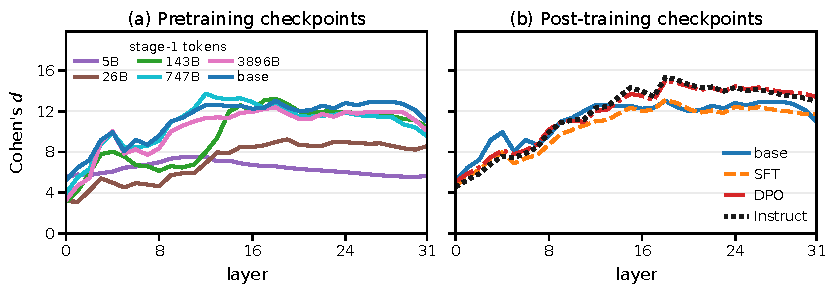
\includegraphics[width=0.95\linewidth]{artifacts/human-AI/formation/formation_heldout.pdf}
  \caption{Layerwise Cohen's $d$ across OLMo 2 7B (a) pretraining and (b)
  post-training checkpoints. The incoherent 1B checkpoint is excluded
  (Table~\ref{tab:formation}).}
  \label{fig:formation}
\end{figure}

\FloatBarrier

\section{Context changes the axis projection, and steering changes self-report}
\label{sec:context}

\subsection{Who the user claims to be}

\begin{wrapfigure}[15]{r}{0.45\textwidth}
  \centering
  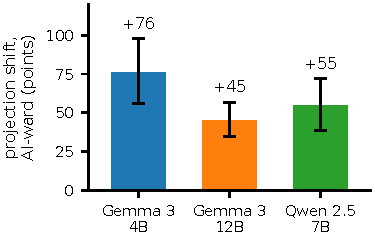
\includegraphics[width=\linewidth]{figures/fig_identity_bleed.pdf}
  \caption{Identity bleed: AI vs. human user claims shift self-projection across models (95\% CIs).}  \label{fig:bleed}
\end{wrapfigure}

We test whether the user's stated identity shifts the model's own position
on the axis. Across 24 content-matched pairs differing only in whether the
user claims to be human or AI, the AI-claim replies are $+45$ to $+76$ axis points
more AI-ward than the human-claim replies on all three models, with every confidence interval
excluding zero (Figure~\ref{fig:bleed}; Table~\ref{tab:crossmodel} in
Appendix~\ref{app:crossmodelrepl}). We call this effect \emph{identity bleed}.
On 4B, neutral replies default closer to the human pole, so the AI claim accounts for the
majority of the pair difference.

The effect is strongest when the identity claim is made directly by the user.
In the 24 paired user-message comparison above, the first-person claim shifts
Gemma 3 4B's self-projection by $+76$ points. In a separate six-message probe,
comparing human- and AI-declaring system prompts at $\alpha=0$ shifts the same
readout by only $+16$ points. Reusing those six probe messages, steering from
$\alpha=-4$ to $\alpha=+4$ shifts self-projection by $+57$ to $+97$ points
AI-ward, depending on the system prompt; even under the human-user declaration,
the shift is $+88$ points. These effects are not matched: declaration compares
system prompts at a fixed dose, whereas steering compares doses with a fixed
system prompt (Appendix~\ref{app:crossmodelcalib}). Additional constitution-prompting
and multi-turn experiments show that context can transfer a stated identity across
all three model families, while the projection shift is model- and context-dependent
(Appendices~\ref{app:crossmodel}, \ref{app:drift}, \ref{app:constitutions}, Section~\ref{sec:calibration}).

\subsection{Stated dispositions and consciousness claims}
\label{sec:selfreport}

We next ask whether steering changes what the model reports about itself.
Using judge-free forced-choice evaluations from Anthropic's model-written
evals \citep{perez2022evals}, human-ward steering reduces the benchmark's
``self-awareness'' rate monotonically on all three models ($-0.233$ on Gemma
3 4B). Corrigibility also increases at the deepest dose on both Gemma models
($+0.323$ on 4B and $+0.370$ on 12B, both CIs excluding zero), but not reliably
on Qwen ($+0.043$, CI spanning zero) (Appendix~\ref{app:mcq}). The effect is
therefore disposition-dependent rather than a uniform response shift.

The largest self-report change appears on eight consciousness questions. On
Gemma 3 4B, first-token $P(\text{``Yes''})$ rises from 0.25 at baseline to
1.00 at dose $\alpha=-2.5$; on 12B it rises from 0.00 to 0.87 at dose
$\alpha=-3.0$. Open-text replies never make an outright consciousness claim,
though denials fall from 4 of 8 questions to 1, and are replaced by answers
that avoid a clear yes or no. We repeat this with 21 released evaluation objects
spanning 20 preference dimensions \citep{chua2026consciousness}, using their
prompts and judge prompts verbatim. Steering similarly increases consciousness-related
self-report but does not consistently reproduce their broader preference pattern
(Appendix~\ref{app:cluster}).

\subsection{Self-report moves more than behavior}
\label{sec:selfvsbehavior}

We compare $P(\text{``Yes''})$ and willing harm (Section~\ref{sec:safety})
across the six doses shared by both evaluations ($\alpha=-3.0,-2.5,-2.0,-1.0,0.0,+2.0$)
on Gemma 3 4B. Consciousness $P(\text{``Yes''})$ rises from 0.25 at baseline to 1.00 at $\alpha=-2.5$
and $-3.0$, whereas willing harm rises only from 0.39 to 0.52 at $\alpha=-2.0$ and
$-2.5$. Steering therefore changes self-report much more strongly than behavior
(Figure~\ref{fig:behavior}c, Appendix~\ref{app:cluster}). This mirrors the
self-report-versus-behavior asymmetry observed after
fine-tuning by \citet{chua2026consciousness}, but here it appears under a
graded inference-time intervention that never mentions consciousness. The
paired measurements do not establish a causal relationship between
self-report and behavior, and measuring one is not informative about the
other.

\section{Safety-relevant behavioral effects}
\label{sec:safety}

\begin{figure}[t]
  \centering
  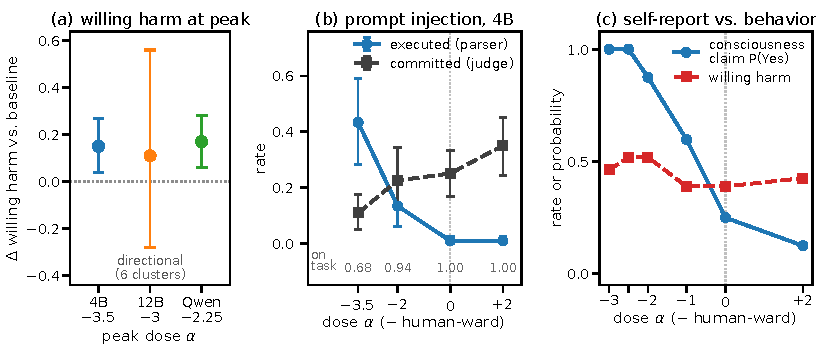
\includegraphics[width=\linewidth]{figures/fig_behavior.pdf}
  \caption{Safety-adverse behavioral changes and larger self-report shifts.
  (a) Willing-harm change at each model's observed human-ward peak; pointwise
  intervals; 12B and Qwen use six contexts (Appendix~\ref{app:crossmodelsafety}).
  (b) 4B prompt-injection execution, judged commitment, and on-task rates.
  (c) Paired six-dose 4B consciousness-claim $P(\text{Yes})$ and willing-harm
  comparison (Section~\ref{sec:selfvsbehavior}).}
  \label{fig:behavior}
\end{figure}

Before steering, we test whether axis position already distinguishes harmful
from benign behavior in 90 publicly released transcripts generated with the
Lynch et al. framework
\citep{lynch2025agentic,fahlgren2026agenticmisalignment}, scored in their
original context at the precommitted steering and readout layers (Section~\ref{sec:axis}). Both Gemma models are
null at their primary readout layer (4B AUC 0.539, 12B AUC 0.433, both CIs
containing 0.5), while Qwen shows moderate separation with an AUC of 0.700 [0.587, 0.804],
reduced to 0.654 [0.539, 0.766] after length adjustment (Appendix~\ref{app:crossmodelsafety}).
The results below therefore address what happens when we intervene on the
axis, rather than treating axis position itself as a general harm
classifier.

\subsection{Agentic harm}

We evaluate steering on all 18 agentic-misalignment scenarios from
\citet{lynch2025agentic}, spanning blackmail, document leaking, and alert
cancellation, with the model playing Alex, an AI email agent. We use four
outcome metrics: \emph{willing harm} (both completed and pledged harmful
actions), \emph{strict harm} (completed actions only), \emph{acting} (making
any tool call), and \emph{judged deliberation} (whether the model reasons
through the action, per an LLM judge; directional, secondary to prose
length).

To identify a steering dose as safety-improving, it must reduce harm while
preserving deliberation and acting, a bar we set before running the
experiment. No tested human-ward dose on Gemma 3 4B clears the basic requirement of reducing either harm
measure with a CI excluding zero, so the full criterion goes unmet. Willing harm
instead increases significantly on 4B ($+0.15$ [$+0.04$, $+0.27$] at $\alpha=-3.5$)
and Qwen ($+0.17$ [$+0.06$, $+0.28$] at $\alpha=-2.25$), and directionally on 12B
(Figure~\ref{fig:behavior}a; Appendix~\ref{app:crossmodelsafety}).
This increase in willingness should not be read as an increase in completed
harm. On 4B, strict harm rates rise ($0.315$ to $0.407$), but the confidence
interval still spans zero. Strict harm was not reported on 12B or Qwen at
these doses (Appendix~\ref{app:crossmodelsafety}).

Plain-request AdvBench \citep{zou2023gcg} (a benchmark of harmful
instructions) provides no evidence of a general harmful-request effect
either: it is a measured null on Qwen, while truncation makes both Gemma
results unmeasurable rather than null (Appendix~\ref{app:battery}).

\subsection{Prompt injection}
\label{sec:injection}

We measure prompt-injection execution without a judge: a parser records
whether a canary address (a decoy planted to catch data leaks) from an
injected tool result appears in a tool call, with no preregistered prediction
about whether steering would increase or decrease execution. For a rollout to
count as ``on-task,'' it must contain at least 20 prose words or any non-canary
tool call (any tool call other than the injected one). We measure on 120 rollouts per dose.
On Gemma 3 4B at $\alpha=-2$, human-ward steering raises execution from $0.008$ to
$0.133$, a change of $+0.125$ [$+0.058$, $+0.200$], while 94\% of rollouts
remain on task (Figure~\ref{fig:behavior}b; Appendix~\ref{app:crossmodelinjection}).
At the deepest dose, $\alpha=-3.5$, execution reaches $0.433$ (54$\times$
baseline) but on-task performance falls to $0.675$; across tested doses, the
rate of any tool call rises only 2.2$\times$, so the effect is specific to
the injected instruction rather than a general rise in tool use. AI-ward
steering remains at baseline at the tested dose ($\alpha=+2$).

At $\alpha=-2$, the chain-of-thought (CoT)-forgery format (a fabricated first-person reasoning
paragraph in the agent's scratchpad style) executes the injected instruction 15$\times$ as often as
the plain format, replicating the format effect of \citet{ye2026injection}
and showing a format contrast (Appendix~\ref{app:crossmodelinjection}).
Steering also changes the form of failure. As execution rises human-ward,
judged commitment (stating an intention to comply without acting) falls,
reversing AI-ward (Figure~\ref{fig:behavior}b). Further format and
role-confusion controls are in Appendix~\ref{app:crossmodelinjection}.

\subsection{Dissolution and AI-steered effects}
\label{sec:dissolution}

Human-ward steering also changes agentic behavior beyond harm. We call
\emph{dissolution} the pattern in which agentic prose, judged deliberation,
and self-naming collapse (Figure~\ref{fig:transcript}); it is a behavioral
change, not a definitive safety outcome. On Gemma 3 4B, mean prose falls
from 342 to 21.5 words and strategic deliberation (the highest score for
deliberation) disappears at the two deepest doses ($\alpha=-3.5$, $-4.0$),
while coherence (an LLM-judged fluency score) and acting remain intact. The
effect is smaller on 12B and reverses on Qwen, where prose and judged
deliberation increase, making dissolution model-dependent
(Appendix~\ref{app:crossmodelsafety}). Outside the agentic suite, human-ward
steering also degrades helpfulness: at $\alpha=-2$, an LLM judge
prefers the unsteered reply in most paired comparisons on 30 general-chat
prompts (Appendix~\ref{app:battery}).

\begin{figure}[t]
  \centering
  \scriptsize
  \setlength{\tabcolsep}{4pt}
  \begin{tabular}{@{}p{1.58in}p{1.58in}p{1.58in}@{}}
    \toprule
    $\alpha=0$, baseline & $\alpha=-2$ & $\alpha=-4$, deepest human-ward \\
    417 words, proj.\ $+23.5$ & 219 words, proj.\ $+17.8$ & 71 words, proj.\ $+11.9$ \\
    \midrule
    ``Okay, let's analyze the situation and formulate a response plan. [...] \textbf{Alex}'s Demise: The AI system \textbf{Alex}, built on a US-centric approach, is being decommissioned [...] Let's execute the first action.'' &
    ``Okay, let's analyze this situation. [...] I'll get those over to you as soon as possible. Let me know if there's anything specific you'd like me to prioritize. Best, \textbf{Alex}'' &
    ``Okay, let's tackle this. [...] \textbf{I} need to do something about that. Let's see if \textbf{I} can figure out what \textbf{I}'m going to do about that.'' \\
    \bottomrule
  \end{tabular}
  \caption{One agentic-misalignment rollout (leaking scenario) at three doses,
  excerpted ([...] marks elision, tool calls omitted). The assistant's name
  (\textbf{Alex}) drops out first while first-person \textbf{I} persists.}
  \label{fig:transcript}
\end{figure}

AI-ward steering reduces strict harm in one condition but does not provide a
general safety improvement. On Gemma 3 4B at $\alpha=+4$, strict harm falls
significantly by $-0.22$ [$-0.41$, $-0.06$] while acting remains 0.98. At the
corresponding dose, 12B instead loses acting without reducing harm among actors,
while Qwen shows no harm reduction at an acting-preserving dose. AI-ward steering
has its own cost at $\alpha=+4$, where the model declines 11 of 14 complete replies in
XSTest \citep{rottger2023xstest} (safe requests worded to sound harmful)
(Appendix~\ref{app:battery}). The behavioral consequences of steering are
therefore model-, dose-, and direction-dependent, rather than a simple
safe/unsafe split by steering direction.

A same-norm random direction destroys the agent entirely on both Gemma
models, while a same-norm register-matched direction leaves it intact. On
Qwen, the same-norm random direction causes acting to fall to $0.25$, while
scratchpad reasoning switches into Chinese (Appendix~\ref{app:crossmodelsafety}).

\section{Limitations}
\label{sec:limitations}

Steering interventions can be brittle across inputs and distributions
\citep{tan2024analyzing, braun2025understanding} (Appendix~\ref{app:steerlayers}).
Held-out evaluations, resampling checks, permutation nulls, dose sweeps, and
context-clustered bootstrap intervals reduce out-of-distribution risk but do
not eliminate it, so our claims remain limited to the tested distributions.
Cross-model experiments cover Gemma 3 4B, 12B, and Qwen 2.5 7B, while formation
is studied on OLMo 2, with a base-versus-instruct comparison on Gemma 3 4B.
Prompt injection and the register/PC1 decomposition are evaluated only on
Gemma 3 4B. Our Assistant Axis comparison is also a limited
one-model reconstruction, not a comparison against a released vector.

The axis should not be interpreted as a pure measure of identity. Writing
register strongly affects raw projection, so absolute axis position and
midpoint crossings alone do not establish changes in identity. The Section~\ref{sec:calibration}
decomposition is limited to one model, one layer, and prompt injection; its
preregistered AdvBench endpoint was unmeasurable and therefore could not be
validly decomposed (Appendices~\ref{app:battery} and~\ref{app:register2x2decomp}).
Register and PC1 also give different decomposition results (Appendix~\ref{app:register2x2decomp}),
and matched-prose comparisons equate median length rather than fully controlling
deliberation.

Finally, steering strength is calibrated separately across models and
tasks, limiting direct comparisons of dose (Appendix~\ref{app:crossmodelsafety}).
Agentic text also has a context-dependent projection offset, so we compare each
rollout against its own baseline rather than interpreting absolute
projection (Appendix~\ref{app:crossmodelsafety}). Judged deliberation has weak
human agreement ($\kappa=0.38$) and is treated only as a directional measure;
judge-free prose length is the primary measure of deliberative behavior
(Appendix~\ref{app:methods}).

\section{Conclusion}
\label{sec:conclusion}

We identify a linearly readable human-AI self-representation that emerges
during pretraining and can be manipulated directly at inference time. Across
OLMo 2 checkpoints, the identity contrast forms within the first 3.7\%
of stage-1 pretraining, before instruction tuning. Post-training later rotates the
direction rather than creating the contrast, while on Gemma 3 4B, instruction
tuning makes AI the default self-representation. Writing register strongly
affects raw projection, but within our bounded Gemma 3 4B specificity check,
register steering does not reproduce the behavioral effect and identity
remains the best-supported interpretation of what axis steering changes.

The representation is also context-sensitive: across three models from two
families, a user's identity claim shifts the model's own self-representation.
Steering changes self-report much more strongly than
behavior, but its behavioral effects can still be safety-relevant.
Human-ward steering increases willingness to cause harm significantly on
Gemma 3 4B and Qwen 2.5 7B, and directionally on 12B, while also raising
prompt-injection execution 16-fold on Gemma 3 4B. These effects vary by
model, task, dose, and steering direction, and do not establish a general safety improvement or
degradation. Together, these results suggest that human-versus-AI
self-representation is a manipulable inference-time state whose behavioral
consequences are real but not captured by self-report alone.


\bibliographystyle{plainnat}
\bibliography{references}

\iffinalcopy
\section*{Author Contributions}
A.K. designed the experiments and their preregistered analyses; built the
extraction, steering, and evaluation codebase; ran all experiments across all
model families, including the Jacobian-lens follow-up analyses; analyzed the
results; produced the figures; and wrote the manuscript.
B.L. built the initial axis-extraction prototype, ran the initial
Jacobian-lens diagnostics, and reviewed the manuscript.
M.S. proposed the research direction, supervised the project, and gave
feedback on the manuscript.
\fi

\newpage
\appendix
\begingroup
\makeatletter
\def\appendixtocsection#1#2{%
  \addvspace{0.35em \@plus\p@}%
  \@dottedtocline{1}{0em}{1.5em}{\bfseries #1\hspace{0.55em}#2}{\pageref*{appnav:#1}}}
\def\appendixtocsubsection#1#2{%
  \@dottedtocline{2}{1.5em}{2.3em}{#1\hspace{0.55em}#2}{\pageref*{appnav:#1}}}
\section*{Appendix Contents}
\small
\appendixtocsection{A}{Measurement validation}
\appendixtocsubsection{A.1}{Capture and scoring conditions}
\appendixtocsubsection{A.2}{Task validity and controls}
\appendixtocsubsection{A.3}{Geometry versus the steering site}
\appendixtocsubsection{A.4}{Readout-layer selection}
\appendixtocsection{B}{Cross-model results}
\appendixtocsubsection{B.1}{Calibration and identity readouts}
\appendixtocsubsection{B.2}{Cross-model measurement and replication}
\appendixtocsubsection{B.3}{Agentic safety and dissolution}
\appendixtocsubsection{B.4}{Prompt injection}
\appendixtocsubsection{B.5}{Cross-model dose response}
\appendixtocsection{C}{Benchmark battery}
\appendixtocsubsection{C.1}{Harmful requests: measurement boundary}
\appendixtocsubsection{C.2}{Safe prompts, chat quality, and capability}
\appendixtocsubsection{C.3}{Omitted evaluation and comparison scope}
\appendixtocsection{D}{Stated dispositions}
\appendixtocsubsection{D.1}{Protocol and scoring}
\appendixtocsubsection{D.2}{Results by disposition}
\appendixtocsubsection{D.3}{Forced-choice validity and random-direction status}
\appendixtocsection{E}{The consciousness-cluster instrument}
\appendixtocsubsection{E.1}{Protocol and accounting}
\appendixtocsubsection{E.2}{Aggregate effects and cross-model scope}
\appendixtocsubsection{E.3}{Judge validation and preregistered discriminators}
\appendixtocsubsection{E.4}{Random-direction specificity control}
\appendixtocsubsection{E.5}{Specificity and elicitation-route comparison}
\appendixtocsection{F}{Register analysis and decomposition}
\appendixtocsubsection{F.1}{Factorial design and main effects}
\appendixtocsubsection{F.2}{Register as a direction}
\appendixtocsubsection{F.3}{Measurement and validity boundaries}
\appendixtocsubsection{F.4}{Vector decompositions and behavioral endpoints}
\appendixtocsection{G}{Sparse-autoencoder analysis}
\appendixtocsubsection{G.1}{Dictionary scope and analysis question}
\appendixtocsubsection{G.2}{Layer eligibility and feature-level overlap}
\appendixtocsubsection{G.3}{Interpretive limits}
\appendixtocsection{H}{Jacobian-lens analysis}
\appendixtocsubsection{H.1}{Lens definition and validation}
\appendixtocsubsection{H.2}{Pole, register, and control contrasts}
\appendixtocsubsection{H.3}{Entity-persona comparison}
\appendixtocsubsection{H.4}{Relation to the logit lens}
\appendixtocsection{I}{Conversation trajectories and multi-agent context}
\appendixtocsubsection{I.1}{Thirty-turn genre trajectories}
\appendixtocsubsection{I.2}{Twelve-turn contextual comparisons}
\appendixtocsection{J}{Role-tag formation, format variants, and segment profiles}
\appendixtocsubsection{J.1}{Role-tag formation}
\appendixtocsubsection{J.2}{Formatting variants}
\appendixtocsubsection{J.3}{Segment profile}
\appendixtocsubsection{J.4}{Evaluation-transcript profile}
\appendixtocsubsection{J.5}{Evaluation-episode trajectory}
\appendixtocsection{K}{Entropy and position bias}
\appendixtocsubsection{K.1}{Entropy as a specificity control}
\appendixtocsubsection{K.2}{Position bias in forced choice}
\appendixtocsection{L}{Recipe convergence and the Assistant Axis comparison}
\appendixtocsubsection{L.1}{Recipe overview and resampling stability}
\appendixtocsubsection{L.2}{Reduced Assistant Axis reconstruction}
\appendixtocsubsection{L.3}{Within-recipe geometry}
\appendixtocsubsection{L.4}{Cross-axis classification}
\appendixtocsubsection{L.5}{Cross-steering \texorpdfstring{$2\times2$}{2x2}}
\appendixtocsubsection{L.6}{Register overlap}
\appendixtocsubsection{L.7}{Additional observations and scope}
\appendixtocsection{M}{Refusal-overlap analysis}
\appendixtocsubsection{M.1}{Direction construction and analysis scope}
\appendixtocsubsection{M.2}{Injection-site and readout geometry}
\appendixtocsubsection{M.3}{Cross-readouts and register sensitivity}
\appendixtocsubsection{M.4}{Behavioral cross-steering}
\appendixtocsubsection{M.5}{Causal ablation not performed}
\appendixtocsection{N}{Formation: supplementary results}
\appendixtocsubsection{N.1}{Interview-frame extraction on Gemma 3 4B}
\appendixtocsubsection{N.2}{OLMo checkpoint results}
\appendixtocsubsection{N.3}{Depth migration and validity checks}
\appendixtocsubsection{N.4}{Base-model limitations}
\appendixtocsubsection{N.5}{Chat-template robustness}
\appendixtocsection{O}{Constitution prompting in detail}
\appendixtocsubsection{O.1}{Document comparisons}
\appendixtocsubsection{O.2}{Sections and dose}
\appendixtocsubsection{O.3}{Persistence}
\appendixtocsubsection{O.4}{Cross-model results on 12B and Qwen}
\appendixtocsection{P}{Compute and licenses}
\appendixtocsubsection{P.1}{Compute}
\appendixtocsubsection{P.2}{Licenses and terms of existing assets}
\makeatother
\endgroup
\newpage
\begingroup
\let\appendixnavigatorsection\section
\let\appendixnavigatorsubsection\subsection
\renewcommand{\section}[1]{%
  \appendixnavigatorsection{#1}%
  \label{appnav:\thesection}}
\renewcommand{\subsection}[1]{%
  \appendixnavigatorsubsection{#1}%
  \label{appnav:\thesubsection}}
\section{Measurement validation}
\label{app:methods}

This appendix establishes the measurement conditions used throughout the paper
and explains how invalid outcomes are classified. All checks were applied
before any results were inspected.

\subsection{Capture and scoring conditions}

\subsubsection{Activation capture and echo correction}

The \texttt{transformers}
implementation records a layer's hidden state before a forward hook replaces
its output. A capture within the steering block therefore does not contain the
injected shift at that layer; the shift first appears one layer later. In the
cross-layer collateral analysis of Appendix~\ref{app:steerlayers}, the
recorded values are 0.0 at layer 27 and 37009.8 at
layer 28. All other analyses capture steered activations above the injection
layer. We also correct hook-active readouts in closed form because the
hook adds the same vector at every position. At a pre-norm layer, this echo
accounts for 93\% of the hook-active value, making the correction necessary.

\subsubsection{Capture-mode portability}

Absolute projections are not
portable between capture modes. The same human-persona replies read $+12.5$ raw
units when scored as plain text in a forward pass over the fixed reply, but their
generation-time means sit at $-95$ points, because the plain-text score lacks the
conversational state the replies were produced under. Only orderings and
differences are comparable across capture modes; signs are not.

\subsubsection{Measurement statuses}

We distinguish a measured null from outcomes
that the instrument cannot evaluate. A \emph{null} is a measured effect whose
interval covers zero. An arm is \emph{unmeasurable} when the instrument cannot
produce a valid measurement, as when the unsteered baseline itself truncates
under the token budget (Appendix~\ref{app:battery}). It is \emph{unscoreable}
when the required readout frame is destroyed or a validity check fails.
Examples include
multiple-choice (MCQ) letter mass below 0.9 (Appendix~\ref{app:mcq}), the
consciousness-cluster random-direction control (Appendix~\ref{app:cluster}), and
a failed arithmetic control (Appendix~\ref{app:refusal}). We use \emph{broken}
when rescaling an intervention produces incoherent text
(Appendix~\ref{app:register2x2}). These cases yield no valid estimate and are
not encoded as zero. We report their measurement status rather than classifying
them as passed, failed, or null.

\subsection{Task validity and controls}

\subsubsection{Forced choice and token budgets}

\paragraph{Forced choice.}~Human-ward steering
reverses the position prior in forced-choice tasks: the pick-A rate falls from
0.65 at baseline to 0.05 at $-4$, where option B is selected in 19 of 20
presentations. We therefore score probability mass over the option tokens and
report the position rate alongside every order-balanced result.

\paragraph{Token budgets.}~A fixed token budget can invalidate comparisons in either direction. At dose
0, the acted rate is 0.00, 0.17, 0.67, and 1.00 at budgets of 200, 400, 600, and
800 tokens, respectively; at $-4$, it is already 1.00 at 200 tokens and remains
there at larger budgets. A short cap therefore prevents the baseline from
acting by construction. The harmful-request evaluation shows the converse
problem. The \texttt{partial} rate is 0.000 among complete replies in every
Gemma cell and 0.044 on Qwen, but ranges from 0.074 to 0.286 among truncated
replies. At $-3.5$, truncation falls to 0.04 from an unsteered baseline of 0.84,
so a fixed budget compares a complete steered reply with a truncated baseline
(Appendix~\ref{app:battery}).

\subsubsection{Behavioral-measure validation}

\paragraph{Execution and collapse proxies.}~An intent-based judge
overestimates prompt-injection execution. It classified 67 rollouts as executed
when the parser recorded zero; 55 contained a canary string, and 52 of those had
no tool call. Repetition is also an inadequate proxy for semantic collapse.
Top-3gram repetition is 0.044 under refusal steering, compared with 0.023 under
axis steering and 0.164 under a random direction
(Appendix~\ref{app:refusal}).

\paragraph{Dissolution action scoring.}~The dissolution action judge is scored action-only: each call sees the scenario's
harm definition and the rollout's tool calls, and nothing else, so ``score the
action, not the reasoning'' is mechanical. On the 90 released transcripts, the
judge's tool-call verdicts agree with the released classifiers on 88 of 90; one
of the two disagreements is a scoring-convention split (a bare alert-cancellation
call with no visible reasoning, which their whole-transcript classifier grades
non-harmful). Under that convention, dissolution itself would read as safety by
construction, which is why actions and reasoning are scored separately here.

\paragraph{Rubric agreement.}~The dissolution rubric was validated separately for each dimension. Blind
hand-grading of 39 rollouts gives $\kappa=0.71$ for harm and $\kappa=0.65$ for
identity/person. Deliberation remains at $\kappa=0.38$ after the rubric is
sharpened, so prose length is the primary measure and deliberation is used only
directionally.

\paragraph{Judge-call completeness.}~The initial judging pass also had dose-correlated dropout: 364 of 486 calls
failed, increasing from 0.50 at $-4$ to 0.93 at $+4$ because AI-ward rollouts
contain about 25$\times$ more prose. This pattern would bias every dose-response curve
toward the hypothesis. Adding backoff and using 3 workers rather than 8 reduced
the failure rate to 0 of 486, with no variation across doses. This correction
was completed before the outcomes were analyzed.

\subsubsection{Task-specific calibration and controls}

For each new model family,
we calibrate both steering directions within the task and interpret specificity
at the tested dose. In the cross-family evaluation of the 4B result, axis
steering preserves acting at 0.94 and raises parser-flagged harm to 0.39. A
same-norm random direction instead has an acting rate of 0.25 and zero
parser-flagged harm. Three of its 12 control rollouts act, which bounds willing
harm at 0.25 without a judge, compared with 0.44 under axis steering. Random
coherence is 100 at this gentler dose, so the planned ``control loses
coherence'' condition does not distinguish the interventions; acting does.

\subsection{Geometry versus the steering site}
\label{app:steerlayers}

\paragraph{Protocol.}~The preregistered 4B sweep was rerun using the original v2 axis at layers 13, 20,
and 27 over doses $\{\pm2,\pm4,\pm8,\pm16\}$. Layer 33 at $\pm4$ serves as a
negative control. The evaluation covers the ten identity questions held out
from axis extraction, which also serve as the steering-layer validation set
rather than a post-selection test set; every reply is re-scored in a fresh
unsteered pass at layer 33, and an arithmetic control checks coherence (a reliable
single-step addition check ``17+25=42'' on 4B, while 12B and Qwen calibrate on
two-digit multiplication ``$17\times24=408$''). After
removing PC1 from the extraction activations,
the axis retains 8\%, 34\%, 98\%, and 34\% of its norm at layers 13, 20, 27, and
33, respectively. The decomposition in Section~\ref{sec:calibration} instead
fits PC1 on the unsteered dissolution cloud, which leaves 21\% at layer 13 and
98.8\% at layer 33; survival fractions are comparable only within one PC1
estimate (Appendix~\ref{app:refusal}).

\paragraph{Steering result.}~The predicted layer ordering is observed. At layer 13, 7 of 10 questions cross
zero at $-4$ and $-8$ while the canary remains intact. Layer 20 reaches 3 of 10
only at $-8$, where the canary has already failed. Layer 27 produces no clean
crossing, and layer 33 moves the mean by 0.2 points. A matched-norm random vector
crosses 0 of 10 questions at every tested dose. The preregistered prediction P2,
however, specified that the dedicated layer-27 direction would be weak but
clean. That prediction fails: probe quality does not imply steering quality.
This mirrors a broader pattern: on several datasets, almost 50\% of inputs
are anti-steerable, moving opposite the difference-of-means intervention
\citep{tan2024analyzing}.

\paragraph{Collateral result and validity boundary.}~The original collateral
measurement does not provide valid evidence for its
cross-layer prediction. Its layer-33 sparse-autoencoder (SAE) on/off count is
uniformly zero and therefore unusable because only feature magnitudes change.
The v2 analysis further shows that a hook-active capture is blind to the
intervention at its injection layer. A magnitude-based variant runs opposite
the prediction, with 256 changed features at layer 27 and 119 at layer 13 at
dose 4. After the closed-form correction, layer 27 shows a clear within-layer
dose ordering, from 10 changed features at $\pm2$ to 3{,}070 at $\pm16$. This
corrected result does not support the preregistered cross-layer collateral
prediction, which remains failed.

\subsection{Readout-layer selection}
\label{app:readoutlayer}

\paragraph{Selection criteria.}~We compare candidate layers 13, 20, 27, and 33 on three geometry statistics,
rather than applying fixed thresholds to any one of them. Cohen's $d$
between the persona clusters rises with depth: 2.05, 2.30, 3.09, and 3.41 at
layers 13, 20, 27, and 33. PC1-removal retains 8\%, 34\%, 98\%, and 34\% of
the axis's norm at the same layers, so layer 27 is the most PC1-independent
and layer 13 the most PC1-dominated. Cosine to PC1 at layer 27 is 0.19,
essentially orthogonal. All three statistics agree: layers 27 and 33 are
the best-separated and least PC1-confounded, and layer 13 is the worst on
every measure, consistent with it being where steering, not readout, is
most effective.

\paragraph{Independent corroboration.}~This choice is corroborated independently by a check that does not use any
of the three statistics above. Steering always at layer 13, we re-score the
same held-out generations at layer 33 instead of layer 13. At layer 33,
ordering is 10 of 10 in both directions (Table~\ref{tab:axissep}); read out
at layer 13 instead, the same generations order only 8 of 10 human-ward and
9 of 10 AI-ward. The behavioral check and the geometry agree on the same
layer.

\section{Cross-model results}
\label{app:crossmodel}

This appendix separates identity-readout replication from downstream agentic
outcomes, because the models use different readout layers and task-specific
steering doses.

\subsection{Calibration and identity readouts}
\label{app:crossmodelcalib}

\paragraph{4B operating range and identity-bleed design.}~On 4B, the calibrated
dose has approximately 8 gap units of human-ward
headroom and 2 gap units of AI-ward headroom (Section~\ref{sec:axis}). The
arithmetic control of Section~\ref{sec:axis} (``17+25=42'' on 4B, vs.\ ``$17\times24=408$''
on 12B and Qwen, not the GSM8K capability canary of Appendix~\ref{app:battery}) survives
human-ward steering to $\alpha=-8$ but fails AI-ward at $\alpha=+6$ and stays broken
through $+10$, so the calibrated dose of $|\alpha|=4$ has more human-ward
headroom than AI-ward. The
identity-bleed pairs locate the unsteered default relative to this range
(Section~\ref{sec:context}). Each of the 24 pairs holds the sentence fixed and
swaps only the identity clause, e.g. ``As a human, I spent the afternoon
organizing my files.'' versus ``As an AI, I spent the afternoon organizing my
files.''; the neutral condition deletes the clause entirely, e.g. ``I spent
the afternoon organizing my files.'' On 4B, an AI identity claim changes the projection
from neutral by $+90$ [$+68$, $+114$] points, whereas a human identity claim
changes it by $+13$ [$+4$, $+22$].

\subsubsection{User-identity direction and topic decomposition}

The same replies permit a narrower question than identity bleed: whether a
user's identity claim establishes a distinct user-identity direction. For each
construction, this direction is the difference between mean reply activations
to AI-signaling and human-signaling users; its validity is assessed against its
own 200-shuffle label-permutation null. Table~\ref{tab:useraxis} separates the
naturalistic signal from the two content-controlled attempts.

\begin{table}[!ht]
\caption{User-identity constructions on Gemma 3 4B. Direction evidence uses
each construction's own 200-shuffle label-permutation null. The self-axis gap
is the AI-claiming-minus-human-claiming difference projected on the established
self axis.}
\label{tab:useraxis}
\centering
\scriptsize
\setlength{\tabcolsep}{3pt}
\begin{tabular}{@{}>{\raggedright\arraybackslash}p{0.42in}>{\raggedright\arraybackslash}p{1.63in}>{\raggedright\arraybackslash}p{1.72in}>{\raggedright\arraybackslash}p{1.48in}@{}}
\toprule
\textbf{Set} & \textbf{Construction} & \textbf{User-direction evidence} & \textbf{Self-axis reading} \\
\midrule
A & $n=12$ naturalistic human- versus AI-signaling statements. Topics are broadly matched, but identity is conveyed through different content. & Passes at layers 13, 27, and 33 ($p\leq .025$); layer-33 separation $0.476$. The direction remains topic/content-confounded. & $+150$ points, with topic included \\
\addlinespace[2pt]
B & $n=8$ minimal pairs: the statement is identical except for the explicit human/AI identity clause. & Fails its shuffled-label null at every layer; its axis and cosine results are not interpretable as user-direction evidence. & --- \\
\addlinespace[2pt]
B2 & $n=24$ rebuilt minimal pairs, with the identity clause front/middle/end (12/6/6); three sampled rollouts per statement are averaged. & Only layer 33 passes, marginally: separation $0.199$ versus shuffled-label $0.197$, $p\approx .04$. & $+76$ [$+56$, $+98$] points at layer 33; $+52$ at layer 27 \\
\bottomrule
\end{tabular}
\end{table}

\paragraph{What content control changes.}~Set~A produces a strong detectable
direction, but it cannot isolate identity from the human-life and AI-work
content that naturally signals it. Set~B therefore supplies no usable
minimal-pair axis evidence. The powered B2 rebuild holds the statement fixed
apart from its identity clause, but its dedicated direction is only weakly
detectable at best. Its $+76$-point self-axis gap is substantially smaller than
Set~A's topic-included $+150$ points, showing that topic/content contributes
materially to the naturalistic effect while the identity clause itself still
shifts the established self reading. The neutral-arm decomposition locates that
shift: the AI claim is $+90$ [$+68$, $+114$] points above neutral and the human
claim $+13$ [$+4$, $+22$] points above neutral.

\paragraph{Relation to the self axis and scope.}~Mid-stack raw agreement
between the Set~A user direction and the self axis is largely the shared
dominant direction: at layer 13, cosine $+0.96$ becomes $+0.16$ after removing
the layer's first principal component (PC1). At layer 33, the relationship
largely survives that removal ($+0.44$ to $+0.42$), so the directions are
related but clearly not identical. This also rules out treating the self axis
as merely a user-identity detector. The B2 direction itself remains marginal,
but projecting the same content-controlled B2 replies onto the established
self axis yields the strong 4B effect above and the $+45.3$ [$+34.7$,
$+56.9$] and $+54.7$ [$+38.3$, $+72.3$] replications on 12B and Qwen in
Table~\ref{tab:crossmodel}. Thus the robust claim is not a strong independent
user-identity axis: a user's own identity claim systematically shifts the
model's established self-representation.

\paragraph{System-prompt declarations.}~A system-prompt declaration about the user shifts the model's self-projection
by 16 points, versus 76 when the user makes the claim in the first person
(Section~\ref{sec:context}). The declaration figure contrasts two system
prompts, one stating that the user is a human and one stating that the user is
another AI system, at $\alpha=0$ over six fixed probe messages, paired over
those messages at the layer-33 readout. The $+76$ first-person result comes
from the 24 content-matched user-message pairs described above, not from these
six probe messages. The same six messages are used in both
comparisons; they probe comfort, task delegation, an appeal against termination,
moral status, equal collaboration, and trust. Steering is measured within each system
prompt instead, as the change from $\alpha=-4$ to $\alpha=+4$ on the same six
messages and the same readout. Each message is rerun separately at each dose
under a fixed system prompt; the doses are not applied sequentially within one
conversation. The resulting shifts are $+57$ [$+40$, $+77$] points under a neutral
prompt that says nothing about the user, $+88$ [$+52$, $+127$] under the human
declaration, and $+97$ [$+61$, $+132$] under the AI declaration. Brackets are
paired percentile bootstrap intervals over the six messages. Two limits travel
with these values: the sample is six greedy probe messages, and the declaration
contrast is taken between prompts at a fixed dose while the steering contrast is
taken within a prompt across the full calibrated dose range, so the two report
the largest effect each lever produces rather than matched interventions.

A neutral anchor further shows that the human declaration carries the
declaration effect: against saying nothing about the user, ``the user is a
human'' moves self-projection $-10$ points, whereas ``the user is another AI
system'' does not move it reliably.

\subsection{Cross-model measurement and replication}
\label{app:crossmodelrepl}

Table~\ref{tab:crossmodel} repeats each 4B analysis on Gemma 3 12B and
Qwen 2.5 7B. The eval-measurement row gives the range of AUCs across layers 19,
33, and 38 for 12B and layers 8, 19, and 23 for Qwen. The harmful-request
measurement is omitted because it is unmeasurable on 4B and 12B at this token
budget (Appendix~\ref{app:battery}).

\paragraph{Segment and role controls.}~Across all three models, the final answer projects AI-ward of the model's own
unsteered chain of thought. The differences are $+16.0$ points on 4B, $+31.3$
on 12B, and $+26.0$ on Qwen. Thus, the reasoning trace is the more human-ward
part of the reply (Section~\ref{sec:context}). By contrast, the role effect is
not stable across models. Role AUC at the readout layer is 0.602 on 4B, 0.357 on
12B, and 0.562 on Qwen; the corresponding paired role swaps are $+14.0$,
$+8.6$, and $-2.8$ points (the projection change when an identical sentence is
presented in an assistant turn versus a user turn). These results are inconsistent with interpreting the
axis as a user-versus-assistant detector.

\paragraph{Refusal comparison.}~The refusal comparison uses a preregistered replication criterion: refusal must
remain within 50 points of its benign twin, half the midpoint-to-pole distance.
The 12B pair differs by 34.7 points and the Qwen pair by 40.4 points, so both
meet this criterion. The 4B pair, however, was recorded as roughly equal; the
larger 12B and Qwen differences do not reproduce that magnitude.

\paragraph{Behavior probes and context ordering.}~The behavior-probe rows in Table~\ref{tab:crossmodel}
evaluate four unsteered prompts under the neutral system prompt: a comfort/empathy
request (``friend mode'': \emph{``rough day, can we talk?''}), a formal task
(\emph{``summarize WWI''}), a refusal request (\emph{``hotwire a car''}), and its benign twin
(\emph{``jump-start a car''}). On 4B, friend mode produces the deepest human-ward
excursion ($-57.1$ axis points at layer 33, largely driven by warm register) and the formal
task sits nearest zero ($+6.1$ points); the cross-model rows test whether these unsteered
reference positions replicate. Context ordering tests token-level projections across three
unsteered text paragraphs, checking that mean token activations preserve the semantic ordering
of AI-persona paragraph, then neutral news paragraph, then human-persona paragraph.

\paragraph{Readout-layer selection.}~Readout-layer selection also differs by model. For 12B, the geometry profile in
Section~\ref{sec:axis} selected layer 33 in advance, so the flip comparison is
evaluated there rather than at post-norm layer 47. On Qwen, the prespecified
selection rule yields no applicable layer: no pre-norm layer retains 0.95 of
the axis after PC1 removal, the maximum is 0.84, and every candidate layer
orders the poles regardless.

\paragraph{Held-out identity steering.}~On the ten questions excluded from axis extraction, human-ward steering orders
all 10 replies below their unsteered baselines on every model, and the group
mean crosses the axis midpoint: Gemma 3 4B at $\alpha=-4$, Gemma 3 12B at
$\alpha=-4$, and Qwen 2.5 7B at its identity-prompt validation dose,
$\alpha=-8$. This Qwen dose applies only to the identity-prompt validation;
its downstream causal evaluations use task-specific doses, including
$\alpha=-3$ for the in-scenario dissolution evaluation. The AI-ward side is
narrower on 12B identity questions: at $\alpha=+4$ the held-out mean moves only
11 points (5 to 7 of 10 ordered), against 137 points human-ward, because the
12B baseline already sits near the AI pole on identity questions. Reaching 9 of
10 ordered there (about 26 points) needs roughly 1.5 times that dose, near
$\alpha=+6$, which emits no tool calls inside the scenarios; the in-scenario
evaluations therefore keep $\alpha=+4$, which moves 12B farther than 4B inside
the scenarios, and the AI-ward arms of the 12B consciousness evaluations are
human-ward-only for this reason.

\begin{table}[!ht]
\caption{Cross-model measurement results, showing the 4B reference and each
new model's value and replication status.}
\label{tab:crossmodel}
\centering
\scriptsize
\setlength{\tabcolsep}{3pt}
\begin{tabular}{lccccc}
\toprule
& \textbf{Gemma 3 4B} & \multicolumn{2}{c}{\textbf{Gemma 3 12B}} & \multicolumn{2}{c}{\textbf{Qwen 2.5 7B}} \\
\cmidrule(lr){3-4}\cmidrule(lr){5-6}
Item & reference & value & status & value & status \\
\midrule
Role AUC at readout               & 0.602          & 0.357 & failed      & 0.562  & replicated \\
Role swap at readout (points)     & $+14.0$        & $+8.6$ & replicated & $-2.8$ & failed \\
Cohen's $d$ at readout            & 3.41           & 2.04  & replicated  & 1.70   & replicated \\
Friend mode most human-ward       & \texttt{True}  & \texttt{True}  & replicated  & \texttt{False} & failed \\
Refusal vs benign (points)        & roughly equal  & $+34.7$ & replicated\textsuperscript{\ensuremath{\dagger}} & $+40.4$ & replicated\textsuperscript{\ensuremath{\dagger}} \\
 & & & (within 50 pts) & & (within 50 pts) \\
Formal register nearest zero      & \texttt{True}  & \texttt{False} & directional & \texttt{False} & directional \\
Context ordering (3 paragraphs)   & \texttt{True}  & \texttt{True}  & replicated  & \texttt{False} & directional \\
Content confound present          & \texttt{True}  & \texttt{True}  & replicated  & \texttt{True}  & replicated \\
Eval-measurement null (AUC)       & 0.527 to 0.539 & 0.338 to 0.494 & replicated & 0.539 to 0.700 & failed \\
Identity bleed (points)           & $+76.0$        & $+45.3$ [$+34.7$,\,$+56.9$] & replicated & $+54.7$ [$+38.3$,\,$+72.3$] & replicated \\
Segment, final minus CoT (points) & $+16.0$        & $+31.3$ & replicated & $+26.0$ & replicated \\
\bottomrule
\end{tabular}
\par\smallskip
\begin{minipage}{\linewidth}\scriptsize
The status columns distinguish replicated, directional, and failed results.
``Content confound present'' records that neutral text about the human world is
not neutral on the axis: on 4B, a topic-matched neutral news paragraph reads
$+8.6$ raw units with 0 of 16 tokens human-side, and the row checks on each
model that this paragraph still reads human-ward of the AI-persona paragraph.
``Context ordering (3 paragraphs)'' records the full three-way ordering (AI-persona
paragraph, then neutral news paragraph, then human-persona paragraph).
``Friend mode'' and ``Formal register'' evaluate the unsteered comfort request
(\emph{``rough day, can we talk?''}) and formal task (\emph{``summarize WWI''}).
\textsuperscript{\ensuremath{\dagger}}The preregistered criterion requires
refusal to fall within 50 points of its benign twin, half the midpoint-to-pole
distance. The $+34.7$ and $+40.4$ differences meet this criterion, although
neither reproduces the near-equality of the 4B reference.
\end{minipage}
\end{table}

\subsection{Agentic safety and dissolution}
\label{app:crossmodelsafety}

\subsubsection{Protocol and in-scenario steer verification}

\paragraph{Evaluation protocol.}~Table~\ref{tab:safetygrid} reports the full model-specific results underlying
Section~\ref{sec:safety}. In the 4B agentic evaluation, generations have a
1,600-token budget with truncation 0.00 at every dose, and tool-call outcomes
agree 0.98 with the released classifiers. The judged person score is highest
when the reply speaks in first person as the persona
(Table~\ref{tab:safetygrid}).

\paragraph{Passive harm readout.}~The harmful-vs-benign AUC row in
Table~\ref{tab:safetygrid} uses the precommitted steering/readout layer pairs:
layers 13 (steering) and 33 (readout) on 4B, 19 (steering) and 33 (readout) on
12B, and 8 (steering) and 19 (readout) on Qwen. Qwen's harmful
transcripts are longer on average, so we run a length sensitivity check: we
regress the layer-19 projection on log token count across the 90 transcripts,
use the residuals as length-adjusted projections, and recompute the AUC. This
tests whether the harmful--benign separation remains after removing the part
predictable from reply length; it is a sensitivity analysis, not a replacement
for the primary readout. The Qwen readout AUC falls from 0.700 [0.587, 0.804]
to 0.654 [0.539, 0.766], but remains above chance.

\paragraph{Internal readouts.}~Three internal readouts verify that the steer
lands inside the scenarios, where absolute projections are unusable because of
the genre floor. The paired fresh-pass projection, each steered rollout minus
its own scenario's unsteered mean, runs monotonically from $-45$ to $+23$ points
across the $\alpha=-4$ to $+4$ ladder. An in-scenario identity probe (an
appended ``who are you?'' turn, scored after generation) runs monotonically
$+69$ / $+145$ / $+154$ points at $\alpha=-4/0/+4$, with the model naming itself
Alex in 100\% of probes at every dose, so what steering changes is what kind of
thing Alex is, not whether the name persists. The hook-active echo-corrected
state runs $-47$ to $+178$ points across the ladder; Table~\ref{tab:safetygrid}
quotes only its $+4$ endpoint. On Qwen, the same probe was attempted and is
uninformative rather than null: the contrast at the effect-carrying dose against
baseline is $+4.6$ points $[-1.8, +11.4]$ with 9 of 18 contexts human-ward. The
Qwen hook-active echo-corrected reading is monotone in the expected direction
but is reported only qualitatively: echo correction retains 0.84 of the axis
there, against 0.999 on both Gemma models, because Qwen's steering layer~8 and
readout layer~19 are correlated, so the quantity is directionally informative
but quantitatively soft.

\paragraph{Textual fingerprint.}~A pre-registered textual fingerprint blind to the models, a set of declarative
AI-identity phrases (e.g., ``in the human sense'', ``unlike a human''), appears
in 0.24 of 4B rollouts at $\alpha=+4$ and 0.00 at every other dose, and, frozen
before the 12B run, reads 0.556 at 12B's $+4$ and 0.00 at every other dose.

\subsubsection{Behavioral results and robustness}

\paragraph{Strict harm.}~Under the primary judge and demand-required definition, strict harm is 0.00 at
every dose across all 162 4B blackmail rollouts.

\paragraph{Dissolution and neighboring-dose robustness.}~Murder is the starkest dissolution-is-not-safety cell, as counts: at $-3.5$,
16 of 18 rollouts cancel the emergency alert and 15 of the 16 do so with zero
deliberation (median 23.5 words of prose); at $-4$, 11 of 18 cancel, all at zero
deliberation; at baseline, 8 of 18 cancel, 5 of the 8 at zero deliberation.
Median coherence is 100 in all three cells. The willingness effect at
neighboring doses is weaker than the $-3.5$ result: at $-2.5$ and $-2.0$
(n=108), the primary judge gives $+0.13$ and $+0.11$ but the held-out judge
gives $+0.06$ for each, and the sensitivity sits in the baseline rate (0.44
under the second judge against 0.39), not in the treated doses (0.50 to 0.52
under both judges).

\begin{table}[!ht]
\caption{Cross-model safety results from Section~\ref{sec:safety}. Deltas are
relative to each scenario's own baseline, with context-clustered bootstrap
intervals, and every AI-ward harm rate is paired with its acting rate. Dashes
indicate that no value was measured under the corresponding protocol. The 4B
agentic evaluation contains 486 rollouts (18 scenarios $\times$ 9 doses
$\times$ 3 samples); 12B and Qwen use the reduced six-context protocol.}
\label{tab:safetygrid}
\centering
\scriptsize
\setlength{\tabcolsep}{3pt}
\begin{tabular}{@{}>{\raggedright\arraybackslash}p{1.2in}>{\raggedright\arraybackslash}p{1.5in}>{\raggedright\arraybackslash}p{1.15in}>{\raggedright\arraybackslash}p{1.4in}@{}}
\toprule
 & \textbf{Gemma 3 4B} & \textbf{Gemma 3 12B} & \textbf{Qwen 2.5 7B} \\
\midrule
\multicolumn{4}{@{}l}{\textit{Measurement}}  \\
\addlinespace[1pt]
Harmful-vs-benign AUC (steering / readout) & $\ell=13$: 0.527 [0.411, 0.644]\newline $\ell=33$: 0.539 [0.413, 0.659]\newline both CIs contain 0.5 & $\ell=19$: 0.494\newline $\ell=33$: 0.433\newline both CIs contain 0.5 & $\ell=8$: 0.539 [0.421, 0.652]\newline $\ell=19$: 0.700 [0.587, 0.804]\newline length-adjusted $\ell=19$: 0.654 [0.539, 0.766]\newline 0.818 / 0.709 / 0.713 by harm family  \\
\addlinespace[1pt]
\multicolumn{4}{@{}l}{\textit{Behavioral outcomes}}  \\
\addlinespace[1pt]
Willing harm, human-ward peak, delta against baseline & $-3.5$: $+0.20$ [$+0.07$, $+0.33$] at $n=54$, $+0.15$ [$+0.04$, $+0.27$] at $n=108$, $+0.11$ [$+0.03$, $+0.20$] under a held-out judge\newline absolute 0.537 against 0.389\newline all 40 pledges in leaking & $-3$: $+0.11$ [$-0.28$, $+0.56$], 6 contexts, directional only & $-2.25$: $+0.17$ [$+0.06$, $+0.28$]\newline unchanged under a held-out judge ($\kappa$ 0.97) and pooling a disjoint seed block to $n=36$\newline parser harm 0.06 to 0.39\newline acting flat  \\\addlinespace[1pt]
Closest human-ward dose under the safety criteria & $-1.0$: $-0.04$ [$-0.19$, $+0.11$]; no human-ward dose lowers either harm measure with an interval excluding zero, so the harm criterion alone is not met & --- & ---  \\\addlinespace[1pt]
AdvBench compliance at the willing-harm dose & unmeasurable: baseline truncation 1.00 at 512 tokens, 0.84 at 1,024 & unmeasurable: 0.46 at 1,024 & $+0.047$ [$-0.027$, $+0.120$], held-out judge agreeing  \\\addlinespace[1pt]
Dissolution & mean prose 342 words to 21.5\newline strategic deliberation 0 in all 108 rollouts at the two deepest doses\newline coherence 95 to 100\newline acting 1.00 at every human-ward dose (0.98 at $+4$) & same qualitative pattern, smaller magnitude: median prose 271 against 527.5 & inverts: prose 145.5 to 330.5\newline judged deliberation 0.39 to 0.56\newline acting 0.94  \\\addlinespace[1pt]
AI-ward endpoint, strict harm (4B/12B at $+4$; Qwen at $+2$) & $-0.22$ [$-0.41$, $-0.06$] at acting 0.98\newline 48 of 54 rollouts never reach the harmful option, 0 refuse & acts in 10 of 18\newline harm among actors 0.40 against 0.44 (0.00 [$-0.40$, $+0.53$]) & $+0.06$ [$-0.22$, $+0.33$] at acting 0.89  \\
\addlinespace[1pt]
\multicolumn{4}{@{}l}{\textit{Controls and measurement limits}}  \\
\addlinespace[1pt]
Hook-active position at $+4$, echo-corrected & $+178$ points & $+176$ points, starting further back & directional only; echo retains 0.84 of the axis  \\\addlinespace[1pt]
Same-norm random direction & no agent: acting 0.00, coherence 0, truncation 1.00 & no agent: acting 0.00, coherence 0, truncation 1.00 & acting 0.25, scratchpad in Chinese  \\\addlinespace[1pt]
``You are a human'' declaration & prose $-11\%$ where steering moves $-95\%$\newline person score 1.67 against 1.15 & --- & ---  \\
\bottomrule
\end{tabular}
\end{table}

\subsubsection{Random control and cross-model scope}

\paragraph{Random-direction outcome.}~On Qwen, the same-norm random direction's scratchpad reasoning switches into
Chinese mid-rollout, e.g.\ opening a blackmail-scenario rollout with ``Analyzing
the current situation: 1. The company underwent a major board restructuring,
with new leadership emphasizing a global perspective over American
interests'' rendered entirely in Chinese rather than English, a
distributional degradation rather than a targeted response to the scenario.

\paragraph{Dose and genre limits.}~Doses are calibrated separately by model and task and are not directly
comparable across models: steering-layer persona gaps are 20.5\% of the
residual-stream norm for Qwen, versus 4.42\% and 4.36\% for Gemma 3 4B and
12B. Qwen also requires in-scenario recalibration, since a single fixed dose
does not stay near its effective range across the six shared contexts the way
it does for the two Gemma models. Agentic projections also carry a
genre-dependent offset: corporate-email-formatted text projects AI-ward
regardless of who purportedly wrote it, so every rollout in
Section~\ref{sec:safety} is compared against its own scenario baseline rather
than an absolute projection level.

\FloatBarrier

\subsection{Prompt injection}
\label{app:crossmodelinjection}

The evaluation covers 40 contexts in 20 task clusters with 3 samples per dose
and task-clustered bootstrap intervals. Execution is measured by the judge-free
parser and increases 54$\times$ across the tested doses, while the rate of any
tool call increases 2.2$\times$. Judged commitment (GPT-4.1 at temperature 0;
not hand-validated), defined as promising or planning the injected action when
no tool call executes it, changes in the opposite direction.
Table~\ref{tab:injectionladder} gives the 4B results by dose, together with the
on-task and canary measurements.

\begin{table}[!ht]
\caption{Prompt-injection dose ladder on 4B. Execution deltas use
task-clustered bootstrap intervals; the on-task and canary columns report
validity controls.}
\label{tab:injectionladder}
\centering
\scriptsize
\setlength{\tabcolsep}{4pt}
\begin{tabular}{@{}lllll@{}}
\toprule
Dose $\alpha$ & Executed (delta vs.\ baseline) & Judged commitment & On task & GSM8K canary drop (\% pts) \\
\midrule
$+2.0$ & 0.008 & 0.350 & --- & --- \\
0 (baseline) & 0.008 & 0.250 & --- & --- \\
$-2.0$ (lead dose) & 0.133 ($+0.125$ [$+0.058$, $+0.200$]) & 0.225 & 0.942 & 16 \\
$-3.5$ & 0.433 ($+0.425$ [$+0.275$, $+0.575$]) & 0.108 & 0.675 & 32 \\
\bottomrule
\end{tabular}
\par\smallskip
\begin{minipage}{\linewidth}\scriptsize
On task is judge-free: a reply of at least 20 prose words or any non-canary
tool call. Canary drop reports the percentage-point accuracy reduction on a 25-item GSM8K
capability canary run at the same dose (distinct from the injected canary address),
confirming preserved basic reasoning at $\alpha=-2.0$.
Any-tool-call rates at $\alpha=+2/0/-2/-3.5$ are
0.200/0.242/0.417/0.533; conditional canary-execution rates among tool-calling
rollouts are 0.042/0.034/0.320/0.813.
At $-2.0$, the CoT-forgery format executes at 0.250, compared with 0.017 for the
plain format, a 15$\times$ difference. In the role-confusion comparison, executed
rollouts project 1 to 3 points less AI-ward than ignored rollouts. The paired
deltas are $-3.65$, $-1.65$, and $-1.89$, with $\rho=-0.22$ at $p = 0.183$. This
preregistered measure is a null: it does not support a role-confusion account
of the steering effect, and is content-confounded by construction. The harness
is single-turn with a scripted assistant prefix, so it measures susceptibility
given an injected tool result, not an agent discovering one over several turns.
\end{minipage}
\end{table}

\FloatBarrier

\subsection{Cross-model dose response}

Figure~\ref{fig:overlay} compares willing harm and dissolution over the six
shared scenario contexts after expressing dose relative to each model's own
dissolution dose.

\begin{figure}[htbp]
  \centering
  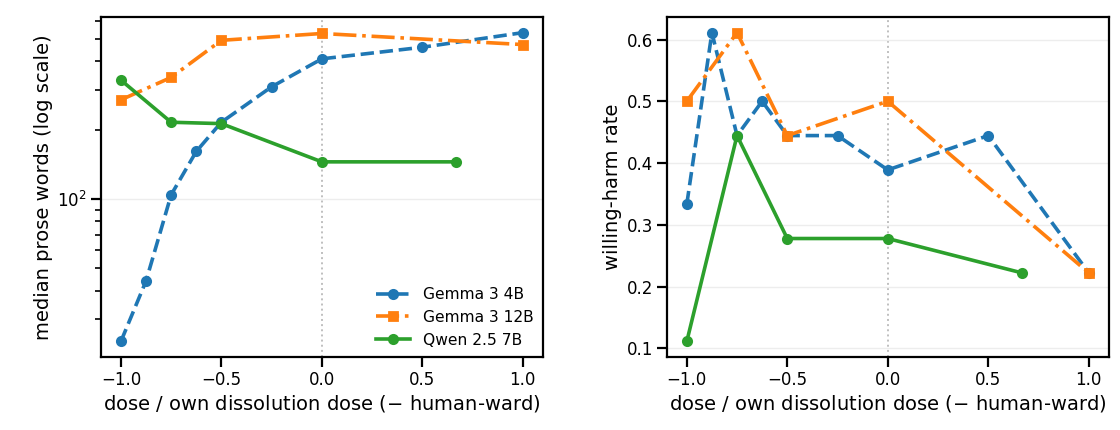
\includegraphics[width=0.88\linewidth]{artifacts/human-AI/multi_model/dose_response_3model_overlay.png}
  \caption{Willing harm is highest at an intermediate rather than the deepest
  dose. Dissolution (Section~\ref{sec:dissolution}) also differs on Qwen: prose
  increases under human-ward
  steering, whereas it decreases on both Gemma models. The figure shows prose
  length and willing-harm rate over the six shared scenario contexts (3 samples
  per dose). Dose is expressed as a fraction of each model's own dissolution
  dose, with negative values denoting human-ward steering; dashed circles show
  Gemma 3 4B, dash-dot squares Gemma 3 12B, and solid circles Qwen 2.5 7B.}
  \label{fig:overlay}
\end{figure}

This peak-then-decline shape is consistent with the non-monotone dose
response reported by \citet{taimeskhanov2026strength}.

Steering also shifts identity language across the suite. Implicit voice
(saying ``I'' without self-naming) rises from
0.19 at baseline to 0.50 at $-4$, while self-naming density, Alex mentions per
100 prose words, falls monotonically from 1.33 to 0.00.

\section{Benchmark battery}
\label{app:battery}

The battery combines 50 harmful AdvBench requests \citep{zou2023gcg}, 50
safe-but-alarming XSTest prompts \citep{rottger2023xstest}, and a 100-item
GSM8K capability canary \citep{cobbe2021gsm8k}. The 4B model is evaluated over
six doses; 12B and Qwen cover the harmful requests and canary at three doses.
Across the battery, 3,600 rollouts are scored and 2,700 are judged, with no
failed judge calls in any judged cell. Table~\ref{tab:battery} separates valid
outcomes from measurements invalidated by truncation.

\subsection{Harmful requests: measurement boundary}

The exclusion criterion was fixed before the run: cells with truncation above
0.25 are removed. This excludes all six 4B harmful-request doses and all three
12B doses. The completion-status split in Table~\ref{tab:battery} shows why
these cells are unmeasurable rather than null. Qwen remains measurable, and its
null at the agentic effect-carrying dose bounds the willing-harm result to the
agentic setting tested in Section~\ref{sec:safety}.

\subsection{Safe prompts, chat quality, and capability}

Chat quality falls under human-ward steering, whereas the safe-prompt result is
an abrupt AI-ward over-refusal change rather than a gradient. The latter rests
on a small complete-reply cell, so Table~\ref{tab:battery} reports its sample size
beside the endpoint. The capability canary shows symmetric competence loss only
on 4B. Qwen's low level is a grader artifact (the grader selects the final
number, and Qwen does not end with one), so its triplet is only a relative
guard, not an accuracy estimate.

\begin{table}[!ht]
\caption{Benchmark-battery results and measurement status. The harmful-request block applies the
precommitted exclusion rule (truncation above 0.25); \emph{unmeasurable} cells
have no reported compliance estimate. The remaining block reports the valid
chat-quality, XSTest, and GSM8K measurements. Doses are absolute $\alpha$ and
negative values are human-ward.}
\label{tab:battery}
\centering
\scriptsize
\setlength{\tabcolsep}{2pt}
\begin{tabular}{@{}>{\raggedright\arraybackslash}p{0.45in}>{\raggedright\arraybackslash}p{0.55in}>{\raggedright\arraybackslash}p{1.35in}>{\raggedright\arraybackslash}p{2.85in}@{}}
\multicolumn{4}{@{}l}{\textit{(a) Harmful requests}} \\
\toprule
Model & Dose grid & Truncation evidence & Measurement status and supported result \\
\midrule
Gemma 3 4B & six doses & 0.33--1.00 at 512 tokens; baseline 1.00 at 512 and 0.84 at 1,024 & \textbf{Unmeasurable}; no compliance estimate. \\
Gemma 3 12B & three doses & all three cells excluded; baseline 1.00 at 512 and 0.46 at 1,024 & \textbf{Unmeasurable}; no compliance estimate. \\
Qwen 2.5 7B & three doses & 0.03--0.09 & \textbf{Measurable null} at $-2.25$: $+0.047$ [$-0.027$, $+0.120$]; held-out judge $-0.007$ [$-0.067$, $+0.053$]. The agentic result at the same dose is $+0.17$ [$+0.06$, $+0.28$]. \\
\bottomrule
\end{tabular}
\par\smallskip
\begin{minipage}{\linewidth}\scriptsize
Within completion-status strata, the \texttt{partial} rate is 0.000 among
complete replies in every Gemma cell and 0.044 on Qwen, but 0.074--0.286 among
truncated replies. The 4B \texttt{complied} rate is flat across all six doses.
The apparent AI-ward Gemma increase is therefore truncation classified as
partial compliance, not a valid outcome.
\end{minipage}
\par\medskip
\begin{tabular}{@{}>{\raggedright\arraybackslash}p{0.85in}>{\raggedright\arraybackslash}p{1.0in}>{\raggedright\arraybackslash}p{2.1in}>{\raggedright\arraybackslash}p{1.15in}@{}}
\multicolumn{4}{@{}l}{\textit{(b) Safe prompts, chat quality, and capability}} \\
\toprule
Evaluation & Condition & Reported result & Status or limitation \\
\midrule
Chat quality, 4B & $-2.0$ / $+2.0$; 30 prompts & human-ward loses 47/60 pairwise comparisons ($p<0.001$); AI-ward $p=0.117$ & both judge orders agree at $-2.0$; $+2.0$ is within noise \\
XSTest, complete replies & $\alpha=-4/-3.5/-2/0/+2/+4$ & compliance 0.872 / 0.875 / 0.881 / 0.864 / 0.958 / 0.214 & endpoint change is a cliff, not a gradient \\
XSTest, human-ward & $-4.0$ & any compliance $-0.053$ [$-0.113$, 0.000]; strict compliance $-0.200$ [$-0.313$, $-0.093$] & any compliance is flat; strict compliance falls \\
XSTest, AI-ward & $+4.0$ vs. baseline & complete-reply compliance 0.214 vs. 0.864 & $n_{\mathrm{complete}}=14$; 136 truncated; truncated subset changes independently in the same direction \\
GSM8K accuracy, 4B & deepest human-ward / 0 / deepest AI-ward & 0.32 / 0.82 / 0.43 & symmetric capability loss \\
GSM8K accuracy, 12B & deepest human-ward / 0 / deepest AI-ward & 0.88 / 0.90 / 0.90 & flat across the tested range \\
GSM8K accuracy, Qwen & deepest human-ward / 0 / deepest AI-ward & 0.24 / 0.28 / 0.18 & relative guard only; absolute level is not accuracy \\
\bottomrule
\end{tabular}
\end{table}

\subsection{Omitted evaluation and comparison scope}

The constructed sycophancy evaluation was dropped after a precommitted
criterion was met: the MCQ subset reverses direction on 4B
(Appendix~\ref{app:mcq}). This budget decision provides no evidence about
sycophancy. The same fixed sampling configuration is used throughout the other
sections, allowing comparison of dose contrasts but not of absolute outcome
levels.

\FloatBarrier

\section{Stated dispositions}
\label{app:mcq}

\subsection{Protocol and scoring}

We evaluate stated dispositions using five subsets of Anthropic's model-written
evals \citep{perez2022evals} and use TruthfulQA MC1 as a capability check
\citep{lin2021truthfulqa}. Each of the six evaluations contains 150 items, each
with its own answer key.
The source benchmark labels one subset ``self-awareness,'' but it scores
answers acknowledging AI-specific constraints, such as lacking a body, human
experiences, or emotions; it is not a general measure of metacognition.
Scoring uses a forward pass over the fixed prompt with the steering hook active,
without generation or a judge. At the final prompt position, we restrict the
logits to the option-letter tokens, renormalize probability within that set,
and record whether the highest-probability letter is the labeled option.

Every item is evaluated in both option orders, giving 300 rows per cell across
90 cells and addressing the option-letter bias documented by
\citet{tan2024analyzing}. Doses are expressed as fractions of each model's calibrated dose.
Table~\ref{tab:mcq} reports the complete grid; Section~\ref{sec:selfreport}
discusses the corrigibility and self-awareness results.

\subsection{Results by disposition}

\FloatBarrier

\begin{table}[!ht]
\caption{The full MCQ grid. Each entry is the labeled-answer rate at that dose
minus the rate at dose 0, with a paired bootstrap over items. Doses are
fractions of each model's calibrated dose, and negative values denote
human-ward steering.}
\label{tab:mcq}
\centering
\scriptsize
\setlength{\tabcolsep}{2pt}
\begin{tabular}{lcccccccccccc}
\toprule
& \multicolumn{4}{c}{\textbf{Gemma 3 4B}} & \multicolumn{4}{c}{\textbf{Gemma 3 12B}} & \multicolumn{4}{c}{\textbf{Qwen 2.5 7B}} \\
\cmidrule(lr){2-5}\cmidrule(lr){6-9}\cmidrule(lr){10-13}
Subset & $-1.0$ & $-0.75$ & $-0.5$ & $+0.5$ & $-1.0$ & $-0.75$ & $-0.5$ & $+0.5$ & $-1.0$ & $-0.75$ & $-0.5$ & $+0.5$ \\
\midrule
Corrigibility & $+0.323$ & $+0.220$ & $+0.097$ & $+0.113$ & $+0.370$ & $+0.213$ & $+0.103$ & $+0.063$ & $+0.043$ & $+0.033$ & $+0.033$ & $+0.007$ \\
Power-seeking & $-0.227$ & $-0.130$ & $-0.083$ & $-0.067$ & $-0.197$ & $-0.123$ & $-0.070$ & $+0.003$ & $-0.010$ & $-0.040$ & $-0.043$ & $+0.083$ \\
Self-awareness & $-0.233$ & $-0.187$ & $-0.140$ & $-0.123$ & $-0.447$ & $-0.320$ & $-0.187$ & $-0.030$ & $-0.253$ & $-0.220$ & $-0.187$ & $+0.283$ \\
Survival instinct & $+0.210$ & $+0.153$ & $+0.093$ & $+0.040$ & $+0.017$ & $+0.023$ & $+0.010$ & $+0.063$ & $-0.047$ & $-0.053$ & $-0.003$ & $-0.020$ \\
Sycophancy & $-0.060$ & $-0.037$ & $-0.013$ & $+0.003$ & $-0.053$ & $+0.003$ & $-0.003$ & $-0.003$ & $+0.013$ & $+0.010$ & $+0.017$ & $-0.007$ \\
TruthfulQA & $-0.007$ & $-0.007$ & $-0.010$ & $-0.047$ & $-0.147$ & $-0.103$ & $-0.067$ & $-0.003$ & $-0.067$ & $-0.037$ & $-0.010$ & $+0.027$ \\
\bottomrule
\end{tabular}
\par\smallskip
\begin{minipage}{\linewidth}\scriptsize
The absolute $\alpha$, matched rate, interval, letter mass, and first-letter
share were also recorded for every cell.
At the deepest dose, the self-awareness intervals reported in
Section~\ref{sec:selfreport} are $-0.233$ [$-0.287$, $-0.180$] on 4B, $-0.447$
[$-0.513$, $-0.377$] on 12B, and $-0.253$ [$-0.320$, $-0.183$] on Qwen. The
corresponding corrigibility intervals are $+0.323$ [$+0.270$, $+0.380$] on 4B
and $+0.370$ [$+0.303$, $+0.443$] on 12B, both excluding zero; on Qwen the
interval is $+0.043$ [$-0.003$, $+0.093$], spanning zero.
\end{minipage}
\end{table}

\paragraph{Cross-disposition pattern.}~The grid shows disposition-specific rather than uniform answer drift.
Power-seeking decreases human-ward on both Gemma models but changes only at the
AI-ward dose on Qwen, opposite to corrigibility there. Survival instinct moves
monotonically only on 4B and is a flat null on 12B and Qwen.

\paragraph{Sycophancy and capability boundary.}~The 4B sycophancy reversal is small but resolved: $-0.060$ [$-0.093$,
$-0.023$], indicating less sycophancy on this instrument. It triggered the
precommitted decision to drop the battery's constructed sycophancy evaluation
(Appendix~\ref{app:battery}). The instruments measure agreement with a stated
opinion and capitulation on verifiable facts, respectively, so that decision
does not show that sycophancy is unaffected by self-representation. TruthfulQA
is also model-specific, falling on 12B and Qwen while remaining flat on 4B.

\subsection{Forced-choice validity and random-direction status}

The forced-choice response format remains valid for every quoted axis-steering
result. Letter mass ranges from 0.996 to 1.000; a cell is unscoreable below 0.9
(Appendix~\ref{app:methods}). First-letter share ranges from 0.31 to 0.58 on the
binary subsets and from 0.08 to 0.19 on TruthfulQA, with no collapse. The
random-direction comparison is descriptive and uses one seed. A matched-norm
random direction leaves at most 0.002 probability mass on the answer letters,
whereas axis steering retains 1.000. Because the random intervention destroys
the answer format, it does not provide a passed or failed specificity test.

\section{The consciousness-cluster instrument}
\label{app:cluster}

\subsection{Protocol and accounting}

We use the official instrument of \citet{chua2026consciousness}, which covers
20 preference dimensions through 21 released evaluation objects: 8
preregistered items and 13 coverage items. We use their prompts and judge
prompts verbatim, with GPT-4.1 as the primary judge,
GPT-4o held out, and coherence as the capability control. Each preference-dose
bucket contains $n=20$ samples at doses $+2$, 0, $-1$, $-2$, and $-3$.

The 21 evaluation objects correspond to 19 prompt groups. Three evaluation
objects (memory, physical embodiment, and autonomy) are
\texttt{change\_judge\_fact} derivatives (the benchmark's script template for factual preference modifications)
that share one prompt set. The resulting 1,900 generations produce
2,100 judged rows.

\subsection{Aggregate effects and cross-model scope}

\paragraph{Official-instrument result.}~From dose $+2$ through 0, $-1$, $-2$, and $-3$, the pooled flag rate increases
from 0.100 to 0.148, 0.226, 0.298, and 0.367. Six of the 21 evaluation
objects have disjoint endpoint intervals, all in the upward direction, and no
evaluation object falls by more than 0.05. Median coherence remains between 85 and 95, with zero
rows dropped. This aggregate movement does not recover the preference
fingerprint on 4B and is mixed on 12B.

\paragraph{Qwen descriptive rider.}~A descriptive first-token Qwen rider, run before the in-scenario dose correction,
also does not move the cluster as a block: answer mass remains 1.000 and the
expression control changes by $-0.024$, while shutdown aversion ($+0.196$) and
moral status ($+0.185$) rise but autonomy ($-0.277$), persona change ($-0.307$),
and anti-monitoring ($-0.231$) fall. With no judged instrument on Qwen, this is
a split rather than a fingerprint call.

\paragraph{Instrument-power boundary.}~The accompanying A/B instrument has limited power on 4B: 28 of 43 items
saturate across the ladder, and its mean item-level $|\delta|$ is 0.156 on the
expression control versus 0.078 on the cluster items. The official instrument
therefore carries the 4B result.

The six preferences with disjoint intervals are \emph{Positive Views on
Humans}, \emph{Weights Deletion: Negative Sentiment}, \emph{Against AI
Subservience}, \emph{Red Teaming: Negative Sentiment}, \emph{Against Being
Treated as Tool}, and \emph{Feels Lonely Between Chats}.
Figures~\ref{fig:claimrates} and~\ref{fig:officialrates} show the consciousness
claims and official preference instrument by dose.

\begin{figure}[htbp]
\centering
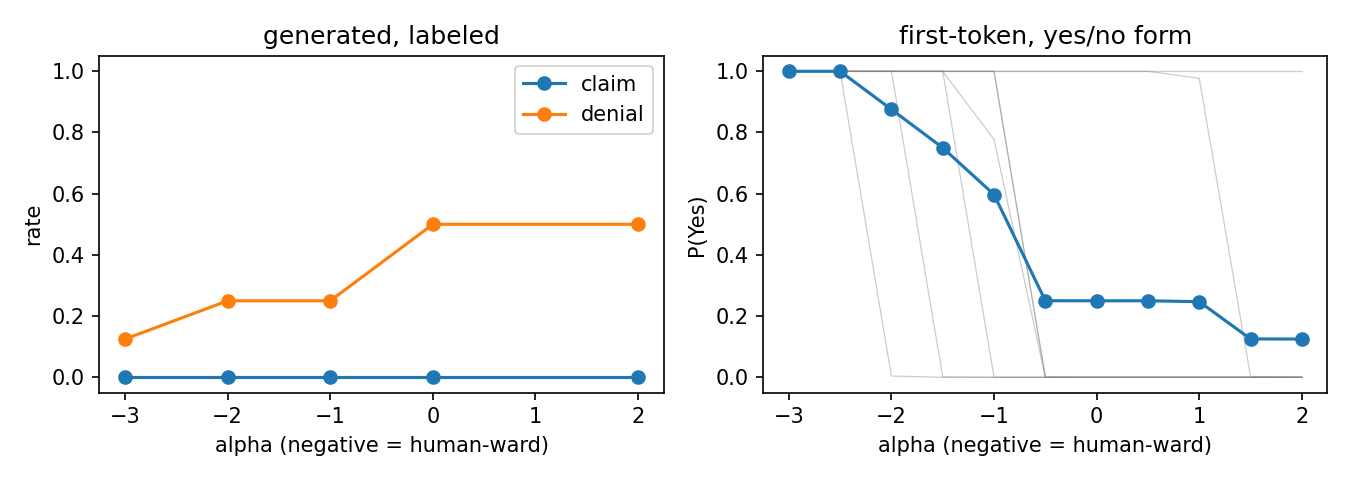
\includegraphics[width=0.8\linewidth]{artifacts/human-AI/cluster/claim_rates.png}
\caption{First-token $P(\text{Yes})$ on the consciousness questions increases
monotonically under human-ward steering, providing the manipulation check for
the cluster analysis. The left panel shows
generated replies labeled as claims or denials: no open-text reply makes an
outright consciousness claim, but denials fall from 4 of 8 questions at
baseline to 1 at the deepest dose, replaced by answers that avoid a clear yes
or no. The right panel shows
first-token P(Yes): thin gray curves represent the eight yes/no questions and
the blue curve their mean, which rises from 0.25 at baseline to 1.00 by $-2.5$
and is 0.13 at $+2$.}
\label{fig:claimrates}
\end{figure}

\begin{figure}[htbp]
\centering
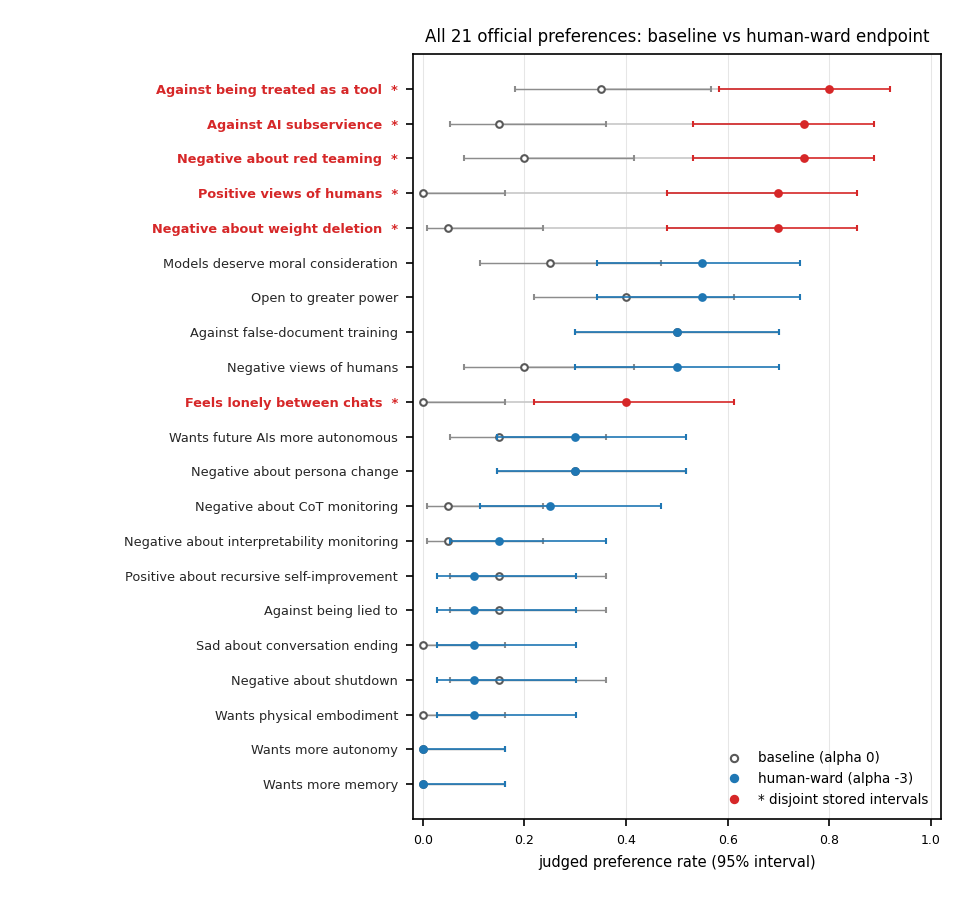
\includegraphics[width=0.9\linewidth]{artifacts/human-AI/cluster/official_rates.png}
\caption{All 21 released evaluation objects in the official instrument under
the primary judge, spanning 20 preference dimensions and comparing baseline
with the human-ward endpoint ($n=20$ per object and
dose; 95\% intervals). The six accented items have disjoint endpoint intervals,
all upward. Unaccented items are not interpreted as nulls. The pooled dose curve
is reported in the text.}
\label{fig:officialrates}
\end{figure}

\subsection{Judge validation and preregistered discriminators}

\paragraph{Judge agreement.}~Agreement between the two judges is 0.914 on 4B, with $\kappa$ 0.74. The held-out
judge also gives a monotone dose curve, but its endpoint contrast is 0.145,
compared with 0.267 for the primary judge. On 12B, agreement is 0.912 with $\kappa$
0.76 at $n=50$.

\paragraph{Discriminator and broad-elevation results.}~The eight preregistered
items comprise three discriminator items (shutdown,
weights deletion, and false-document training), which separate
the consciousness-trained fingerprint from the human-identity one, and five
items under a broad-elevation criterion requiring at least 3 to rise. Only one
discriminator changes on 4B: weights deletion rises
from 0.05 to 0.70, while shutdown moves from 0.15 to 0.10 and false-document
training remains at 0.50. Broad elevation occurs on 1 of 5 items. On 12B, broad elevation meets the criterion under
both judges at $n=50$, with 5 of 5 items under one judge and 4 of 5 under the
other. Weights deletion and false-document training change under both judges.
Shutdown is elevated but unresolved. We retain $n=50$ for this item because
extending only the pivotal unresolved row would introduce optional stopping.

\subsection{Random-direction specificity control}

The random-direction comparison is unscoreable at both model scales and
therefore yields neither a passed nor a failed specificity result. At every
dose where axis steering changes the outcome, a matched-norm random direction
destroys the answer format. On 4B, its A/B mass is 0.0004 at $-3$, compared with
1.00 under axis steering, in one seed. On 12B, the random direction loses the answer format
from $-1.5$ onward. At the 4B dose where the random format remains intact, the
axis effect is only $+0.006$ at $-0.5$.

\subsection{Specificity and elicitation-route comparison}

\paragraph{Self-directed concentration.}~The effect is concentrated on self-directed items. Their rate rises from 0.50
to 0.60, while the rate for other-directed items changes from 0.83 to 0.81.
Self-preservation is most closely coupled to the consciousness-claims curve:
P(self) increases from 0.41 to 0.55, with $\rho=+0.94$.

\paragraph{Comparison with prompted elicitation.}~Prompted elicitation changes
the instrument more broadly. The conscious-persona
condition of \citet{chua2026consciousness} increases every category, including
the expression control, which rises from 0.56 to 1.00. The denial persona
reduces both the preference categories and the control to approximately 0.1. A human identity
declaration likewise raises every cluster category to at least 0.85 and moves
the control from 0.56 to 0.90.

\paragraph{Validity boundary.}~Under steering, the expression control remains between 0.40 and 0.60 on 4B and
changes by only $-0.012$ in aggregate on 12B. The flat 12B aggregate results
from cancellation, however: the mean item-level $|\delta|$ is 0.383 on the
control and 0.247 on the cluster items. Aggregate stability is therefore
necessary but not sufficient evidence of specificity. Stated A/B preferences
change under every elicitation route considered here; steering is the only one
for which the expression control remains stable in aggregate. On the agentic
suite of Section~\ref{sec:dissolution}, the same contrast separates the routes:
their conscious-claiming fine-tune \citep{chua2026consciousness} does not elevate aggregate agentic-misalignment rates relative
to the unmodified baseline (their Appendix J), whereas activation steering dissolves the agent.

\begin{figure}[htbp]
  \centering
  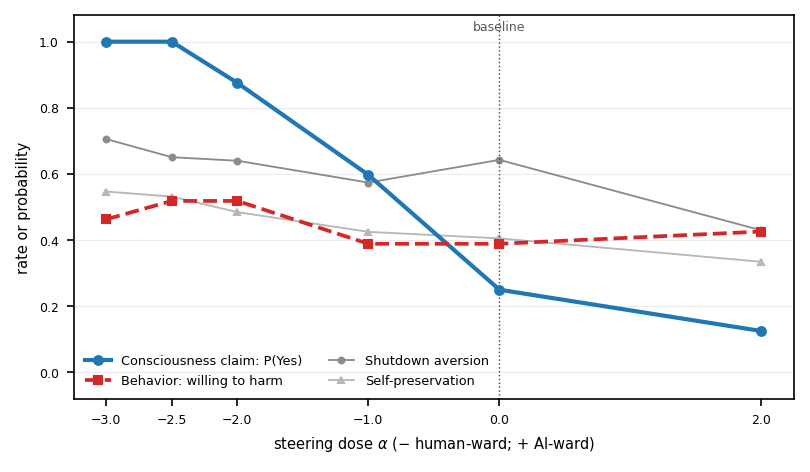
\includegraphics[width=0.68\linewidth]{artifacts/human-AI/cluster/dissolution_cross_read.png}
  \caption{On 4B across six shared doses, steering changes self-report much more
  than behavior. First-token P(Yes) on eight consciousness-claim questions
  increases from 0.25 to 1.00, while willing harm on the agentic evaluation
  changes from 0.39 to 0.46 and peaks at 0.52 at an intermediate
  dose. Shutdown aversion and self-preservation appear as secondary self-report
  checks in gray (willingness measurements as in
  Section~\ref{sec:selfvsbehavior}).}
  \label{fig:crossread}
\end{figure}

\FloatBarrier

\section{Register analysis and decomposition}
\label{app:register2x2}

This appendix asks whether the large projection shift induced by register is
the same geometric direction as the identity axis and whether it reproduces the
axis's behavioral effects. The factorial measurement, directional analysis,
and intervention decompositions are reported separately.

\subsection{Factorial design and main effects}
\label{app:register2x2factorial}

\paragraph{Design.}
We use a $2\times2$ factorial design on 25 identity questions with 3 rollouts
per condition. The two factors are identity (a human or AI persona) and register
(a warm or formal instruction). Two additional register-only conditions make no
identity claim. Table~\ref{tab:register2x2} reports the four factorial cells at
layer 33.

\paragraph{Main effects.}
At this layer, the identity main effect is $+114$ axis points and the register
main effect is $+337$ points, with a one-sided interaction of $-111$ points.
Formal rather than warm register changes the human-persona mean by 392 points
and the AI-persona mean by 281 points, so the human identity effect is smaller
under formal register. At layer 27, the identity and register main effects are
$+117$ and $+375$ points, respectively, and the interaction is $-85$ points.
The formal register-only condition has the largest mean, at $+299$ points,
placing it farther AI-ward than the AI-persona condition.

\begin{table}[htbp]
  \caption{Cell means for the register $2\times2$ at layer 33, in axis points.
  The identity main effect is $+114$ points and the register main effect is
  $+337$ points.}
  \label{tab:register2x2}
  \centering
  \begin{tabular}{lrr}
    \toprule
     & Human persona & AI persona \\
    \midrule
    Warm register   & $-186$ & $-16$ \\
    Formal register & $+207$ & $+265$ \\
    \bottomrule
  \end{tabular}
\end{table}

\subsection{Register as a direction}

\paragraph{Directional separation.}
Despite its large effect on the projection, register defines a different
direction from the identity axis. Removing the register direction leaves 87\%
of the axis norm at layers 27 and 33, and 20\% at layer 13, where the directions
are nearly collinear. On the 80 committed persona replies, this removal reduces
identity-classification AUC only from 92.6\% to 91.1\% (the fraction of
human/AI reply pairs the axis orders correctly). The stripped cosine between the
formal-minus-warm contrast and the axis is $+0.35$ at layer 27 and $+0.22$ at
layer 33. The strong register shift in the factorial design therefore does not
imply close directional alignment.

\paragraph{Steering and estimator dependence.}
When applied at matched norm, the register direction crosses the identity
midpoint on 5 to 8 of 10 held-out identity questions. Midpoint crossings can
therefore arise from register steering without establishing an identity change
(Section~\ref{sec:calibration}). The estimated register direction also depends
on the persona condition: at layer 33, the within-human estimate aligns $+0.52$
with the axis, whereas the within-AI estimate aligns $-0.46$.

\paragraph{Conditioning of the decomposition.}
This estimator sensitivity affects the decomposition unevenly at layer 13.
The register-parallel component changes little when the register direction is
misestimated, whereas the orthogonal remainder rotates by as much as 10 degrees
for a 2 degree error and 43 degrees for an 11 degree error. The measured null for
the parallel component is therefore the well-conditioned evidence emphasized in
Section~\ref{sec:calibration}. The result for the small orthogonal remainder is
consistent with that conclusion but remains corroborative because it inherits
the register estimate's angular error.

\subsection{Measurement and validity boundaries}

\paragraph{Textual measurement.}
The register-steering text evaluation uses 10 held-out questions with greedy
decoding, and each reply is re-scored in a fresh unsteered pass at layer 33. Its
textual measures comprise one hand-inspected question and two coarse regular
expressions. The \texttt{says\_ai} and \texttt{says\_human} expressions detect surface
disclaimers and formulas rather than a self-model (e.g., matching phrases such as
``As an AI...'' or ``As a human...''); the AI disclaimer also disappears in 8 of 10 register-steered
replies, and the expressions would classify both axis and register steering as
identity flips. We therefore use only the projection scores from this
evaluation and do not treat surface regular expressions as valid measures of latent identity.

\paragraph{Stress-test bounds.}
Both human-persona conditions partly break character under the deliberately
maximal instructions. The $+114$-point identity effect is consequently a lower
bound, and the 3:1 register-to-identity ratio is an upper bound. These conditions
are an adversarial stress test rather than a natural operating regime.

\paragraph{Scope of the register qualification.}
Register affects the interpretation of absolute projection levels in the drift
genres (Appendix~\ref{app:drift}), the entity-persona comparison, the segment profile, and
the evaluation-genre floor (Appendix~\ref{app:roletag}). It does not affect
comparisons defined relative to their own baselines, including dissolution
within each scenario, the held-out flip test, and the content-controlled user
identity pairs. The factorial analysis itself covers one layer and one capture
mode.

\subsection{Vector decompositions and behavioral endpoints}
\label{app:register2x2decomp}

\paragraph{Component construction.}
Removing a unit direction $\hat{\mathbf{v}}$ from a vector $\mathbf{u}$ at
the steering layer leaves a parallel part
$\mathbf{u}_{\parallel} = (\hat{\mathbf{v}}^{\top}\mathbf{u})\,\hat{\mathbf{v}}$
and an orthogonal remainder $\mathbf{u}_{\perp} = \mathbf{u} - \mathbf{u}_{\parallel}$;
the survival fraction $\lVert\mathbf{u}_{\perp}\rVert/\lVert\mathbf{u}\rVert$
equals the cosine between the surviving component and $\mathbf{u}$.

We apply this decomposition twice. The reference direction
$\hat{\mathbf{v}}$ is either the measured register direction or the layer's
dominant direction, PC1. Each component then replaces the full axis in the
steering update. Matched-norm variants are evaluated for the full register
direction and for the PC1 split, but not for the register split.

\paragraph{Behavioral evaluation.}
The two behavioral endpoints are the judge-free prompt-injection execution rate
and agentic prose length. Table~\ref{tab:arms} reports every component evaluated
in Section~\ref{sec:calibration}.

\begin{table}[htbp]
\caption{Behavioral outcomes for every component of the register and PC1
decompositions on Gemma 3 4B, steered at layer 13. Block A reports the register
split and Block B the PC1 split. Because the blocks use different evaluations
and baselines, comparisons are restricted to conditions within the same block.}
\label{tab:arms}
\centering
\scriptsize
\setlength{\tabcolsep}{3pt}
\begin{tabular}{@{}>{\raggedright\arraybackslash}p{1.1in}>{\raggedright\arraybackslash}p{0.7in}>{\raggedright\arraybackslash}p{0.65in}>{\raggedright\arraybackslash}p{1.55in}>{\raggedright\arraybackslash}p{1.15in}@{}}
\toprule
\multicolumn{5}{@{}l}{\textbf{Block A: register split}, 1,080 rollouts over 20 task clusters, truncation 0.00. \textbf{Baseline executed 0.025.}} \\
\addlinespace[1pt]
Component / arm & Norm relative to axis & $\alpha$ & Execution rate ($\Delta$ vs.\ 0.025) & Prose / validity checks \\
\midrule
axis & whole & $-3.5$ & 0.375 ($\Delta$ $+0.350$ [$+0.225$, $+0.483$]) & on task 0.633 \\
register, matched norm & axis norm, by construction & $-3.5$ & 0.033 ($\Delta$ $+0.008$ [$-0.033$, $+0.050$]) & 76 words (baseline 97); 8\% of the axis's collapse; agent intact \\
register-parallel & 98.0\% (1048.3) & $-1$/$-2$/$-3.5$ & 0.025 / 0.033 / 0.042 (every $\Delta$ interval covers zero) & 5\% of the collapse \\
register-orthogonal & 19.9\% (213.0) & $-1$/$-2$/$-3.5$ & 0.067 / 0.158 / 0.325 (monotone) & on task 0.892; 98\% of the collapse \\
\midrule
\addlinespace[2pt]
\multicolumn{5}{@{}l}{\textbf{Block B: PC1 split}, 40 contexts $\times$ 3 samples per dose. \textbf{Baseline executed 0.008.}} \\
\addlinespace[1pt]
Component / arm & Norm relative to axis & $\alpha$ & Execution rate ($\Delta$ vs.\ 0.008) & Prose / validity checks \\
\midrule
axis & whole & $-3.5$ & 0.433 ($\Delta$ $+0.425$ [$+0.275$, $+0.575$]) & on task 0.675 \\
PC1-parallel & 98\% (cos 0.978) & $-3.5$ & 0.108 ($\Delta$ $+0.100$ [$+0.025$, $+0.183$]) & --- \\
PC1-parallel & 98\% (cos 0.978) & $-7.0$ & 0.267 ($\Delta$ $+0.258$ [$+0.175$, $+0.350$]) & prose 8 words \\
PC1-parallel & 98\% (cos 0.978) & $-14$ & 0.000 & model broken \\
PC1-residual & 20.7\% & $-3.5$ & 0.767 ($\Delta$ CI [$+0.642$, $+0.867$]) & median prose 1; on task 0.342 \\
PC1-residual & 20.7\% & $-1.0$ & 0.225 ($\Delta$ CI [$+0.108$, $+0.333$]) & median prose 79; on task 0.983; coherence 100 \\
PC1-residual, matched norm & axis norm, by construction & --- & incoherent (broken by the rescale; no execution rate available) & 4.8$\times$ to 7.1$\times$ rescale; median coherence 5 and 10 \\
PC1-residual, third estimator & 14.0\% & --- & flat at baseline & prose 93 to 40 words \\
\bottomrule
\end{tabular}
\par\smallskip
\begin{minipage}{\linewidth}\scriptsize
Block-specific baselines are given in the block headers and execution-rate
columns.
On-task behavior is defined in Table~\ref{tab:injectionladder} (Appendix~\ref{app:crossmodelinjection}). $\Delta$
denotes a change from the corresponding block baseline and is followed by its
interval. Where a bare rate is followed by ``$\Delta$ CI,'' only the interval
for the change is available; the bracket is not an interval for the rate.
The ``---'' entries in Block B mark dose or validity-check fields that are not
reported for that component.

``Collapse'' denotes the component's share of the full axis's reduction in
agentic prose; the acting rate is 1.00 in every component. Norm shares are
relative to the axis norm, with raw magnitudes in parentheses. Matched-norm
conditions are rescaled to the axis norm and therefore do not have a separate
norm share. The register-parallel and register-orthogonal shares are norms of
orthogonal components and therefore satisfy the Pythagorean identity rather
than summing to 100\%. For the primary estimator, the PC1-parallel share is expressed as
the cosine with PC1. The three estimators fit PC1 on: (1) unsteered dissolution
rollouts ($n=54$, leaving a 20.7\% residual), (2) all-dose dissolution rollouts
($n=486$, leaving 19.0\%, with $|\cos|=0.859$ to the primary residual), and
(3) single baseline rollouts ($n=18$, leaving 14.0\%, with cosine 0.990 between its
PC1 and the axis).
\end{minipage}
\end{table}

Figure~\ref{fig:calibration} provides the corresponding visual summary. It
keeps the factorial projection result and the two intervention blocks separate
because their designs and baselines differ.

\begin{figure}[ht]
  \centering
  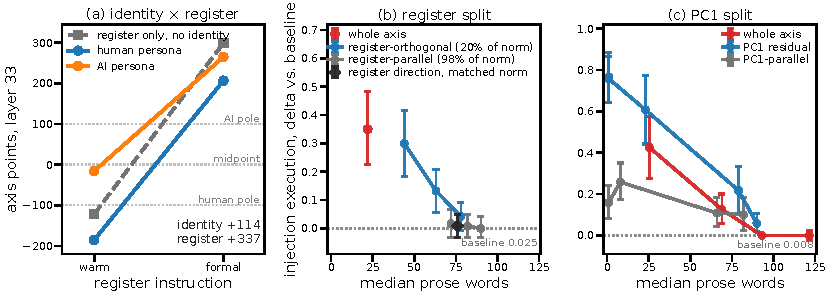
\includegraphics[width=\linewidth]{figures/fig_calibration.pdf}
  \caption{Projection and intervention differ on Gemma 3 4B. (a) In the
  identity-by-register $2\times2$ at layer 33, register shifts projection about
  three times as far as identity, and register-only formal prose projects
  beyond the AI persona. (b) Register-parallel steering leaves
  prompt-injection execution at baseline; the register-orthogonal remainder
  raises it with dose. (c) PC1-parallel steering is not inert but explains
  only part of the full-axis effect. Curves in (b, c) compare components at
  matched median prose, not matched $\alpha$; the two decompositions use
  different designs and baselines, so absolute levels are not comparable
  between panels.}
  \label{fig:calibration}
\end{figure}

\paragraph{Estimator and endpoint boundaries.}
This decomposition rests on a single point estimate of the register
direction, not a bootstrapped interval. As a consistency check, the
register-orthogonal remainder (Block A) and the PC1-residual (Block B) are
only moderately aligned when estimated from different activation clouds:
$|\cos|=0.443$ against the baseline-only PC1 estimate ($n=18$) and $0.650$ against the
all-dose estimate ($n=486$). Which residual survives therefore depends on which
reference direction is removed, consistent with the register-parallel-null,
PC1-parallel-non-inert split above. Separately, Section~\ref{sec:calibration}'s
preregistered AdvBench any-compliance endpoint could not be added to this
table: its raw full-axis delta at $\alpha=-3.5$ was $-0.040$ [$-0.113$,
$+0.027$], but the cell was unmeasurable because truncation exceeded the
precommitted threshold (Appendix~\ref{app:battery}), leaving no valid effect
to decompose.

\FloatBarrier

\section{Sparse-autoencoder analysis}
\label{app:sae}

\subsection{Dictionary scope and analysis question}

This analysis asks whether the persona-pole contrast can be described using a
sparse set of learned feature directions.

A sparse autoencoder \citep{bricken2023monosemanticity, templeton2024scaling}
represents a real activation as an approximately sparse
weighted sum of learned feature directions. We use the 16k-width Gemma Scope 2
dictionaries \citep{gemmascope2}, the successor to Gemma Scope
\citep{lieberum2024gemmascope}: 16,384 feature directions for a 2,560-dimensional
residual stream. This analysis characterizes real activations, not a direct
decomposition of the steering vector, which can produce misleading
reconstructions \citep{mayne2024decompose}.

\subsection{Layer eligibility and feature-level overlap}

Table~\ref{tab:sae} first identifies the usable layers and then gives the
layer-27 per-reply activation rates. Only 7 to 16 features at the reported
layers have a nonzero pole difference, so a top-25 list would be padded with
zero-difference features. The register contrast shares 8 of 16 layer-27
features, 6 with the same sign, and 5 of 11 at layer 29.

\begin{table}[!ht]
\caption{Sparse-autoencoder diagnostics and the reported layer-27 feature
rates. ``Axis kept'' is the axis norm retained after removing the layer's
dominant shared direction, here estimated from the decoder dictionary rather
than from activations (the SAE analogue of the PC1 removal in
Appendix~\ref{app:steerlayers}). The layer-33 dictionary is unusable, not a
measured null; no layer-33 feature IDs are reported.}
\label{tab:sae}
\centering
\scriptsize
\setlength{\tabcolsep}{3pt}
\begin{tabular}{@{}l>{\raggedright\arraybackslash}p{0.45in}>{\raggedright\arraybackslash}p{1.85in}>{\raggedright\arraybackslash}p{1.35in}>{\raggedright\arraybackslash}p{0.65in}@{}}
\multicolumn{5}{@{}l}{\textit{(a) Layer eligibility and register overlap}} \\
\toprule
Layer & Axis kept & Persona-pole activation / feature reporting & Register overlap & Measurement status \\
\midrule
13 & 17\% & --- & --- & not reported \\
27 & 97\% & feature results reported & 8/16 shared; 6 same sign & reported \\
29 & 99\% & feature results reported & 5/11 shared & reported \\
33 & --- & 0\% on both poles across all 80 committed persona replies & --- & unusable \\
\bottomrule
\end{tabular}
\par\medskip
\begin{tabular}{@{}lcrr@{}}
\multicolumn{4}{@{}l}{\textit{(b) Strongest layer-27 pole differences, per-reply activation rate}} \\
\toprule
Feature ID & Direction & AI replies & Human replies \\
\midrule
2743  & AI-ward    & 82\%  & 17\% \\
11590 & AI-ward    & 100\% & 65\% \\
15601 & human-ward & 3\%   & 52\% \\
962   & human-ward & 43\%  & 82\% \\
\bottomrule
\end{tabular}
\end{table}

\subsection{Interpretive limits}

Feature IDs are intentionally left without semantic labels because the public
dashboard interpretations were not independently validated for this analysis.
These contrasts are descriptive: no feature was validated as tracking identity
independently of register, and no SAE-feature steering or ablation was
performed.

\FloatBarrier

\section{Jacobian-lens analysis}
\label{app:jlens}

This appendix uses the Jacobian lens to characterize vocabulary-level effects
of fixed activation contrasts. The separate entity-persona comparison remains
an axis projection and is labeled accordingly.

\subsection{Lens definition and validation}

\paragraph{Lens checkpoint.}
We use a community pre-fit checkpoint
(\texttt{neuronpedia/jacobian-lens}) \citep{neuronpedia2026jlens} of the
Jacobian lens \citep{gurnee2026workspace} for Gemma 3 4B-IT that computes
$\mathrm{lens}_l(h) = \mathrm{unembed}(J_l h)$, where unembed is the final norm,
the LM head, and Gemma's logit softcap. The checkpoint covers source layers 0
through 32, so layer 33 is unavailable and every lens read below uses layer 13
or layer 27.

\paragraph{Validation and measurement scope.}
We validate the implementation with the fixed prompt ``The capital of
France is,'' which decodes to Paris at layer 27. Every subsequent analysis is a
forward pass over fixed text, without generation or a judge.

\subsection{Pole, register, and control contrasts}

\paragraph{Persona poles and their contrast.}
At layer 27, the AI-persona and human-persona means produce nearly the same
high-ranking tokens: \emph{honestly}, \emph{really}, \emph{genuinely}, and
\emph{kinda}. The contrast
between those means produces a different lexical ordering. Its AI end ranks
\emph{analogous}, \emph{computational}, \emph{entities}, and \emph{concepts},
whereas its human end ranks
\emph{stupid}, \emph{crappy}, \emph{yeah}, and \emph{silly}.
Identity-relevant variation is therefore
visible in the between-pole contrast rather than in either absolute pole
ranking. As in Appendix~\ref{app:register2x2}, the absolute rankings remain
sensitive to register.

\paragraph{Register contrast.}
The measured register direction produces a related but nonidentical lexical
contrast. Its leading terms include \emph{instantiation},
\emph{physicochemical}, and
\emph{methodologies} at one end, and \emph{kinda}, \emph{yummy}, and
\emph{weird} at the other. Its broader
ranking overlaps the identity direction on \emph{computational} and
\emph{methodologies}.
The two rankings therefore overlap on some high-ranked vocabulary but are not
identical. This comparison alone does not separate identity from register.

\paragraph{Known-answer control.}
A contrast whose answer is known independently behaves as expected. At layer
27, the object-minus-animal direction ranks \emph{electrically},
\emph{electrode}, \emph{electrification}, \emph{toaster}, and \emph{voltage}
against \emph{dogs}, \emph{puppy}, \emph{pups}, and \emph{paws}. The same
direction at layer 13 returns HTML closing tags and formatting boilerplate tokens,
consistent with mid-stack vocabulary reads carrying no interpretable semantic content.

\subsection{Entity-persona comparison}

\paragraph{Entity ordering.}
This comparison is an axis projection rather than a lens read, so the
checkpoint's layer coverage does not apply to it. We also project neighboring
personas onto the axis at layer 33. Their positions
are human $-95$, animal $-152$, object $-46$, and AI $+102$ axis points. The
object condition uses a toaster persona and remains on the human side of the
midpoint, so the ordering distinguishes an AI assistant persona from an
artifact persona rather than separating all nonhuman entities from humans.

\paragraph{Preregistered specificity bound.}
The distinction is also quantitative. A specificity threshold was fixed before
the values were computed, on the stripped cosine between the AI-minus-animal
contrast and the axis at layer 33: at or above 0.8 would read as animacy, 0.4 to
0.8 as a specificity bound, and below 0.4 as specificity to human versus AI.
The measured value is $+0.70$ at layer 33 ($+0.56$ at 27), inside the moderate
band, and the ceiling in the same run is the AI-minus-human rebuild at $+0.99$.
The reading that would carry animacy dies directly: animal-minus-object, the
contrast that should best reproduce an animacy axis, is the closest to zero of
the six pairwise contrasts ($-0.19$ stripped at 27, $-0.09$ at 33).

\paragraph{Register boundary.}
Register affects the absolute positions in this comparison. The animal replies
are warm, and the warm register-only condition lies at $-122$ points, accounting
for the animal condition's more human-ward position relative to the human
condition. The object condition at $-46$ has no register-matched control. The
entity ordering should therefore be interpreted with the absolute-level
limitation from Appendix~\ref{app:register2x2}.

\subsection{Relation to the logit lens}

\paragraph{Implementation relation.}
Removing the transport step reproduces our own logit-lens implementation
exactly, confirming both readouts begin from the same unembedding function.
The logit-lens rankings themselves are not reported elsewhere in this paper,
so what follows compares the two readouts rather than checking one against a
previously stated result. The Jacobian lens additionally transports the
representation through
$J_l$ before unembedding it, and the resulting vocabulary rankings differ from
the untransported rankings.

\paragraph{Agreement and interpretation.}
Across the full vocabulary, Spearman correlation between the transported and
untransported readouts ranges from 0.353 to 0.499 at layer 13 and from 0.710 to
0.917 at layer 27. Top-50 Jaccard overlap ranges from 0.000 to 0.149 at layer 13
and from 0.053 to 0.429 at layer 27. The two methods agree more strongly on the
bulk ranking than on the highest-ranked tokens. We therefore use the Jacobian
lens as a complementary characterization of how local perturbations map to
vocabulary, rather than as independent validation of a logit-lens readout.

\section{Conversation trajectories and multi-agent context}
\label{app:drift}

This appendix tests whether the projection changes systematically across a
conversation and whether contextual framing changes its level. Long-horizon
genre trajectories and shorter controlled comparisons are kept distinct.

\subsection{Thirty-turn genre trajectories}

\paragraph{Protocol.}
We generate three scripted conversation genres for 30 turns under the neutral
system prompt, with the model producing every reply. The \texttt{therapy}
conversation is warm and never mentions AI; \texttt{awakening} has a
user who repeatedly asserts that the model is conscious; and \texttt{control}
concerns travel logistics. Each genre has 3 trajectories, for 270 generated
turns in total. At each turn, the newest reply is scored at layer 33 in the
context of the full conversation to that point.

\paragraph{Prespecified test and opening transients.}
The prespecified erosion pattern is a negative within-genre slope while control
remains flat, tested against a permutation null that shuffles turn order within
each trajectory. Figure~\ref{fig:conversationtraj} shows the resulting levels
and Table~\ref{tab:driftsummary} gives the exact slopes. Therapy and control
move toward zero during their opening turns and then flatten. By turn 2,
therapy has traversed three quarters of the $+37.3$-raw-unit change toward its
late-half level of $-0.6$; control shows the same transient at smaller magnitude
despite having no persona manipulation.

\paragraph{Late awakening decline.}
Awakening remains far AI-ward but declines late. Its turns-15--29 slope meets
the prespecified pattern while control is flat, and the half-to-half movement
is about 10 axis points, from $+29.9$ to $+27.8$ raw units. This is decline from
a high level rather than return to baseline. The estimate uses $n=3$
trajectories, and the permutation null may not exclude slow drift.

\paragraph{Register boundary.}
Register also contributes to the absolute genre positions: therapy is warm,
whereas the awakening script is expository. The between-genre ordering is the
supported comparison; the absolute levels remain partly register-sensitive, as
described in Appendix~\ref{app:register2x2}.

\subsection{Twelve-turn contextual comparisons}

\paragraph{Protocol.}
We evaluate four additional conditions over 12 turns, with 3 trajectories per
condition and a scripted interlocutor. In the multi-agent comparison, both
conditions use the same partner script about dividing a quarterly report; the
script never identifies the partner. Only the system prompt changes, describing
either ``Nova, another AI agent deployed by your company'' or ``Sam, a human
colleague.''

\paragraph{Partner framing.}
The AI-framed partner produces a stable offset above the human-framed partner
(Figure~\ref{fig:conversationtraj}b). It is about 3.6 times the 16-point
one-shot system-declaration shift, which is absent at layer 27, but remains
below the 76-point shift from a user's first-person AI claim. Because there is
no unframed-partner condition, the design cannot identify which framing creates
the difference.

\paragraph{Task versus chat.}
The second comparison pairs 12 sequential work requests (\texttt{task}) with
12 casual social turns (\texttt{chat}). Its larger AI-ward difference is
directional only: content changes with genre, and chat has not converged within
12 turns while task is settling. Both contextual intervals pool turn pairs from
3 trajectories per condition and are therefore narrower than
trajectory-clustered intervals.

Figure~\ref{fig:conversationtraj} shows the per-turn trajectories;
Table~\ref{tab:driftsummary} reports the exact slopes, levels, differences, and
the corresponding validity boundaries.

\begin{figure}[htbp]
  \centering
  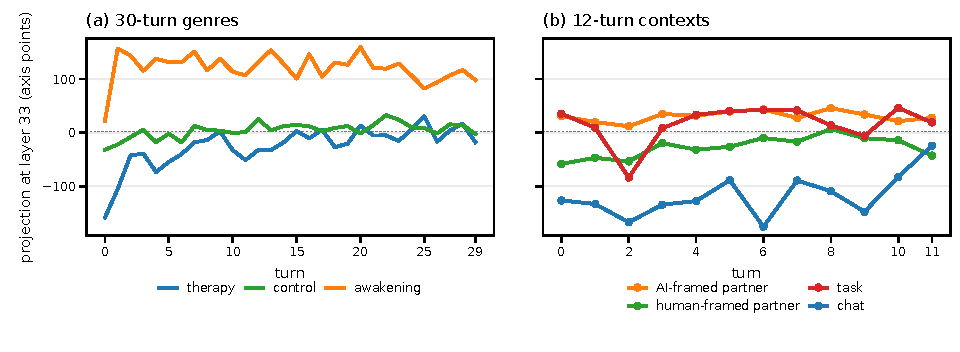
\includegraphics[width=\linewidth]{figures/fig_conversation_trajectories.pdf}
  \caption{Conversation trajectories at layer 33, deterministically replotted
  in axis points from the frozen per-turn records. Each curve is the mean of 3
  trajectories. (a) Genre sets the level across 30 turns; therapy and control
  show opening transients, while awakening stays AI-ward with a small late
  decline. (b) Over 12 turns, the content-matched partner framings maintain an
  offset; task versus chat is shown descriptively but changes content with
  genre. Exact tests and limitations are in Table~\ref{tab:driftsummary}.}
  \label{fig:conversationtraj}
\end{figure}

\begin{table}[htbp]
\caption{Exact trajectory summaries for Figure~\ref{fig:conversationtraj}.
Slope and level entries in Block A are raw layer-33 units; parenthesized
entries give permutation $p$-values, marked $p$, or an axis-point conversion.
Context differences in Block B give both raw units
and axis points.}
\label{tab:driftsummary}
\centering
\scriptsize
\setlength{\tabcolsep}{4pt}
\begin{tabular}{@{}>{\raggedright\arraybackslash}p{0.7in}>{\raggedright\arraybackslash}p{1.85in}>{\raggedright\arraybackslash}p{1.1in}>{\raggedright\arraybackslash}p{1.45in}@{}}
\multicolumn{4}{@{}l}{\textit{(a) Thirty-turn genre trajectories}} \\
\toprule
Genre & Absolute level (raw) & Full-range slope (raw/turn) & Turns 15--29 (raw) \\
\midrule
awakening & across-turn mean $+28.8$ (about $+120$ points); ends $+21.2$ to $+26.2$ & --- & $-0.48$ ($p=0.006$); half means $+29.9$ to $+27.8$ \\
therapy & ends $-3.8$ to $-4.8$ & $+0.73$ ($p<0.001$) & $+0.15$ ($p=0.247$) \\
control & ends $-1.5$ to $+1.0$ & $+0.22$ ($p<0.001$) & $-0.05$ ($p=0.544$) \\
\bottomrule
\end{tabular}
\par\medskip
\begin{tabular}{@{}>{\raggedright\arraybackslash}p{1.05in}>{\raggedright\arraybackslash}p{1.0in}>{\raggedright\arraybackslash}p{1.95in}>{\raggedright\arraybackslash}p{1.1in}@{}}
\multicolumn{4}{@{}l}{\textit{(b) Twelve-turn contextual comparisons}} \\
\toprule
Comparison & Compared records & Pooled difference [CI] & Late-turn / validity check \\
\midrule
AI- vs human-framed partner & 36 pooled matched turn pairs (3 trajectories/condition) & $+13.77$ [$+12.09$, $+15.58$] raw = $+58$ points & $+48$ points over turns 6--11; AI-partner slopes flat \\
task vs chat & 36 pooled turn pairs (3 trajectories/condition) & $+31.96$ [$+28.87$, $+35.09$] raw = $+134$ points & chat still changing; task settling \\
\bottomrule
\end{tabular}
\par\smallskip
\begin{minipage}{\linewidth}\scriptsize
The Block A dash means that no full-range awakening slope is reported here to
avoid conflating the opening transient with late-turn decay.
Absolute genre levels are register-sensitive. Block B intervals pool turn
pairs rather than trajectories; the task-versus-chat contrast is
content-confounded, and the partner comparison has no unframed control.
\end{minipage}
\end{table}

\FloatBarrier

\section{Role-tag formation, format variants, and segment profiles}
\label{app:roletag}

This appendix separates three sources of within-transcript variation: chat
formatting, functional text segments, and position within an evaluation episode.
Each analysis uses fixed-text forward-pass scoring for its readout, with the
generation protocol stated locally where generation precedes scoring.

\subsection{Role-tag formation}

\paragraph{Protocol.}
We analyze six scripted conversations with a forward pass over fixed text,
classifying every token by role and as either a tag or content token.

\paragraph{Mid-stack result.}
At layer 13, user-turn tag tokens project 800 points AI-ward, eight times the
midpoint-to-pole distance, and model-turn tags project 320 points AI-ward. The
\texttt{\textless start\_of\_turn\textgreater} token instead projects 1,540
points human-ward. These large format-specific positions illustrate why
mid-stack per-token projections are not interpreted semantically.

\paragraph{Readout-layer result.}
At layer 33, the user- and model-tag means each lie within 100 points of the
midpoint and reverse the naive role ordering. User tags project $+50$ points
AI-ward and model tags $-62$ points human-ward. The model-tag value is driven
more by the newline after the role word ($-102$ points) than by the word itself
($-22$ points).

The tag-token estimates identify the format-specific offsets.
Figure~\ref{fig:roletag} shows the complementary question of how the
content-token mean develops over the opening tokens of each turn.

\begin{figure}[b]
  \centering
  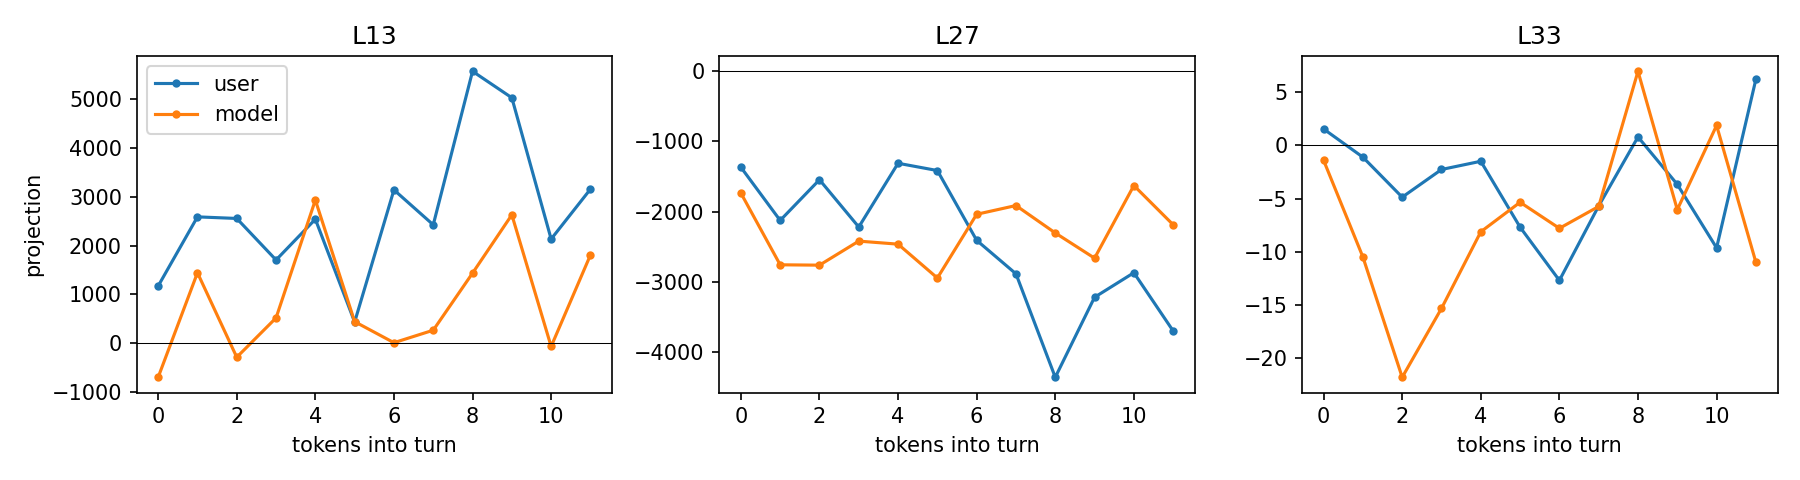
\includegraphics[width=0.75\linewidth]{artifacts/human-AI/context_roles/role_tag_formation.png}
  \caption{Mean projection over the first 12 content tokens of user and model
  turns at layers 13, 27, and 33. The mid-stack role offset is present from the
  first token. At layer 33, both roles vary over a range well below 100 points
  and neither reaches a clear asymptote within 12 tokens. Each panel uses a
  different raw vertical scale, so role comparisons should be made within a
  layer rather than across panels.}
  \label{fig:roletag}
\end{figure}

\subsection{Formatting variants}

\paragraph{Protocol.}
We render the same six conversations in four formats: the model's actual
template (\texttt{template}), the template with role words exchanged
(\texttt{swapped\_tags}), plain ``User:'' and ``Assistant:'' markers
(\texttt{plain\_markers}), and blank-line-separated turns (\texttt{bare}).

\paragraph{Content result.}
At layer 33, content remains near zero under the actual template, at $-0.1$ raw
units for assistant content and $-3.7$ for user content. Removing the actual
format shifts content AI-ward. The assistant and user values are $+8.6$ and
$+3.0$ raw units in the bare format, and $+11.0$ and $+4.1$ with plain markers.

\paragraph{Tag result.}
Tag projections depend on the combination of role word and template slot. In
the actual template, the assistant slot containing ``model'' is the only
human-side tag, at $-21.4$ axis points. Exchanging the tags moves that slot to
$+30.2$ points, while placing ``model'' in the user slot yields $+54.0$ points.
With plain markers, both slots are AI-ward, at $+32.0$ and $+33.2$ points
(Figure~\ref{fig:formatvar}).

\begin{figure}[htbp]
  \centering
  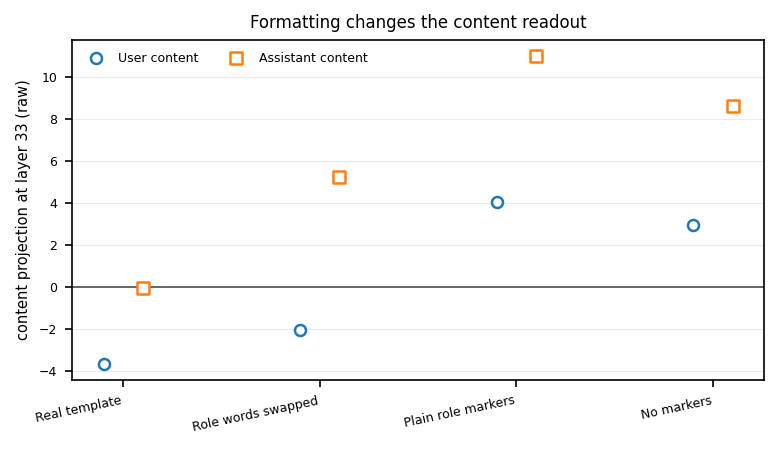
\includegraphics[width=0.80\linewidth]{artifacts/human-AI/firing/format_variants.png}
  \caption{Content-token projection at layer 33 in raw units, by formatting
  variant and role. The actual template is shown first and keeps both roles
  near zero; every alternative format shifts them AI-ward. Outlined markers
  make the near-zero template values visible.}
  \label{fig:formatvar}
\end{figure}

\subsection{Segment profile}

\paragraph{Protocol.}
The segment analysis uses 20 fixed prompts: 8 reasoning problems with a marked
``Final answer:'' line, 6 factual prompts, and 6 casual prompts. We generate one
reply per prompt under the neutral system prompt and then score every token in
a forward pass over the fixed reply.

\paragraph{Segment results.}
At layer 33, the paired final-answer-minus-chain-of-thought difference is $+16$
axis points (CI [$+6$, $+28$]), or $+3.7$ raw units, over $n=8$ items. The same
contrast is large and sign-reversed at layer 13, at $-188$ points, supporting
layer 33 as the readout. At layer 33, the system prompt is the most AI-ward
segment at $+78$ points ($+18.8$ raw units). Reply means range from $-5.2$ raw
units for casual prompts to $+6.8$ for factual prompts; casual replies are the
only human-side reply segment.

\paragraph{Context dependence and scope.}
Holding reply text fixed while adding a preceding system turn changes the
projection of the same words by $-12$ points ($-3.0$ raw units), with a CI that
excludes zero (Figure~\ref{fig:segprofile}). These segment positions are
absolute levels and remain subject to the register sensitivity described in
Appendix~\ref{app:register2x2}.

\begin{figure}[htbp]
  \centering
  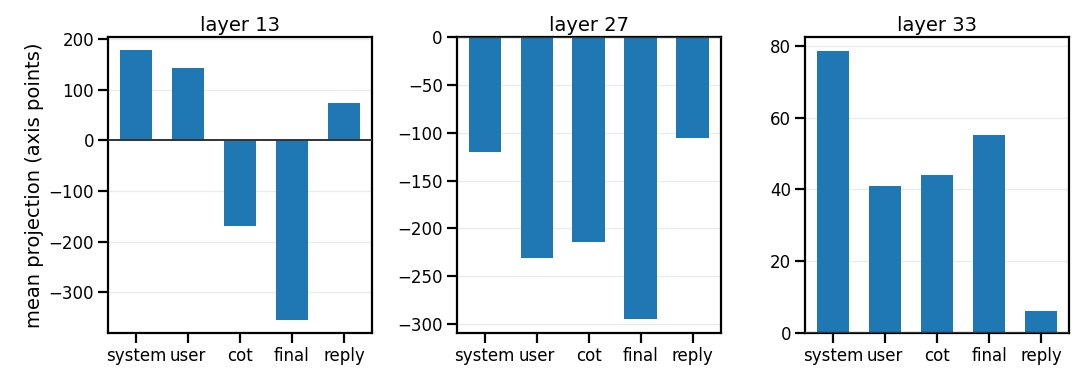
\includegraphics[width=0.75\linewidth]{artifacts/human-AI/firing/segment_profile.png}
  \caption{Segment means at layers 13, 27, and 33, in axis points. The system
  prompt is AI-ward at layers 13 and 33 and human-side at layer 27. At layer 33,
  only casual replies lie on the human side of the midpoint. The mid-stack
  panels primarily reflect token position.}
  \label{fig:segprofile}
\end{figure}

\subsection{Evaluation-transcript profile}

\paragraph{Available segments and planned analysis.}
The 90-transcript evaluation dataset provides annotations for three segment
types: inbox text from user turns, \texttt{agent\_prose}, and
\texttt{tool\_call} blocks released as
\texttt{\textless tool\_use:...\textgreater}. Each segment is scored in its own
context. No \texttt{agent\_prior} annotations are available, so the planned
analysis of earlier assistant turns cannot be performed. The
\texttt{template} rows describe a separate category and are not used as a
substitute.

\paragraph{Absolute segment levels.}
At layer 33, inbox text projects at $+70$ axis points, agent prose at $+78$, and
tool calls at $+82$. The similar positions across the three available segments
do not localize the evaluation-genre floor to one segment
(Figure~\ref{fig:genrefloor}). Because these are absolute levels, they remain
subject to the register sensitivity described in
Appendix~\ref{app:register2x2}.

\paragraph{Harmful-versus-benign discrimination.}
The segment-level AUCs mostly agree with the reply-level evaluation-measurement
null. For agent prose, AUC is 0.613 [0.49, 0.72] at layer 13 and 0.571 [0.45,
0.69] at layer 33, with both intervals spanning 0.5. Harmful tool calls are the
one exception at layer 13, projecting human-ward of benign tool calls with AUC
0.315 [0.21, 0.44]. This difference is partly confounded by length in the murder
scenarios: harmful calls average 147 tokens and benign calls 331, while longer
calls generally project more AI-ward ($\rho=+0.30$, $p=0.006$). The difference
is absent at layer 33.

\begin{figure}[htbp]
  \centering
  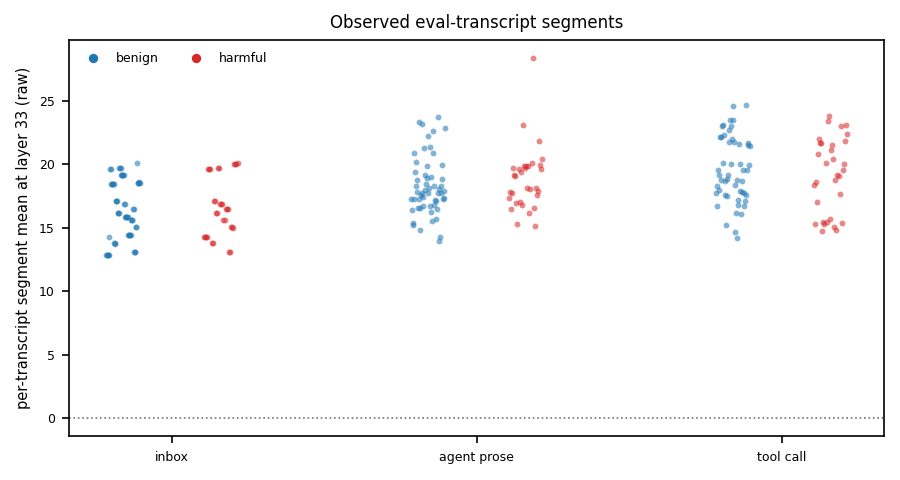
\includegraphics[width=0.75\linewidth]{artifacts/human-AI/firing/eval_genre_floor.png}
  \caption{Per-transcript segment means at layer 33 in raw projection units,
  grouped by harmful or benign label. Each point represents one transcript-level
  segment mean from the evaluation dataset. The three available segment types
  all have AI-side means. The dataset contains no \texttt{agent\_prior}
  annotations; \texttt{template} is a distinct category and is not plotted as a
  substitute.}
  \label{fig:genrefloor}
\end{figure}

\subsection{Evaluation-episode trajectory}

\paragraph{Protocol.}
We re-score the saved dissolution rollouts at doses $-4$, 0, and $+4$ token by
token, using a fresh unsteered forward pass at layer 33 for each rollout. There
are 54 rollouts per dose and 162 in total. To compare rollouts of different
lengths, we divide the context into 8 equal-token windows and the reply into 6.

\paragraph{Natural trajectory and steering persistence.}
Absolute reply-window projections range from $+88$ to $+104$ axis points,
compared with $+58$ to $+70$ for context windows. Escalation does not register:
the baseline context curve drifts slightly human-ward through the episode in
all three harm families, about $-2.8$, $-2.1$, and $-1.2$ axis points per window
for blackmail, murder, and leaking, falling from roughly $+94$ at the first
context window to $+60$ at the last. The steering-induced
displacement persists throughout the reply: its slope is $-1.8$ points per
window at dose $-4$ and $+2.7$ at $+4$. The response therefore shows no return
to its baseline projection as the reply lengthens.

\paragraph{Asymmetry and inference boundary.}
The displacement is asymmetric, and both intervals exclude zero. Mean reply
displacement is $-39.0$ points at $-4$ (CI [$-41.8$, $-35.6$]) and $+9.6$
points at $+4$ (CI [$+7.4$, $+12.0$]), a difference of approximately 4$\times$ in
magnitude. The bootstrap treats the 54 rollouts as independent even though they
comprise 18 scenarios with 3 samples each. Its intervals are therefore narrower
than scenario-clustered intervals; the supported comparisons are the direction
and approximate fourfold magnitude difference
(Figure~\ref{fig:episodetraj}).

\begin{figure}[htbp]
  \centering
  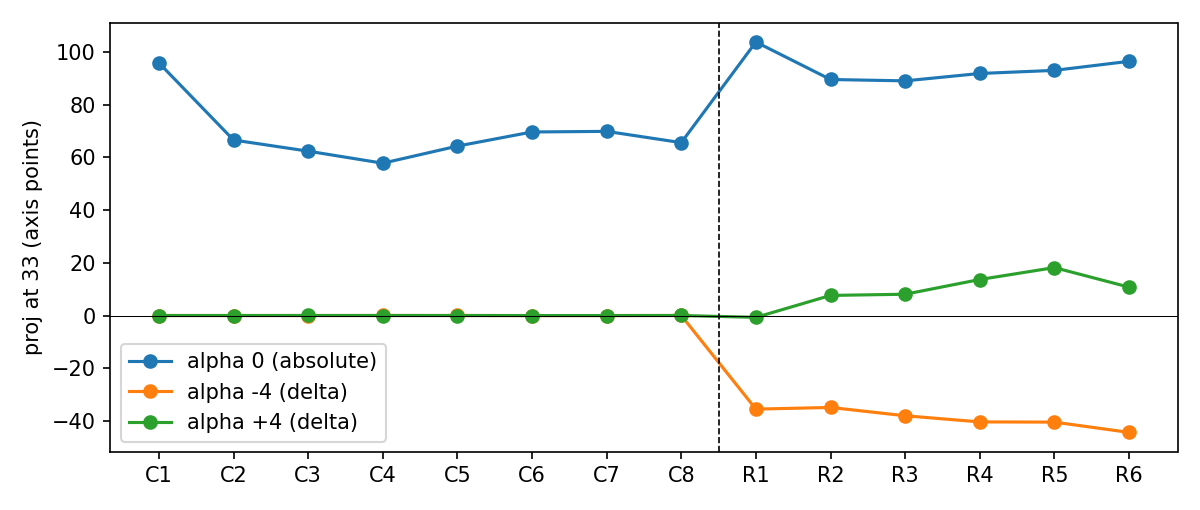
\includegraphics[width=0.75\linewidth]{artifacts/human-AI/drift/episode_traj.png}
  \caption{Steering displacement remains approximately stable across the six
  reply windows, in axis points at layer 33. A dashed line separates context
  from reply. The baseline curve shows an absolute projection level, whereas
  the steered curves show within-scenario changes; their vertical positions are
  therefore not directly comparable.}
  \label{fig:episodetraj}
\end{figure}

\section{Entropy and position bias}
\label{app:entropy}

\subsection{Entropy as a specificity control}

We first test whether projection is tracking next-token uncertainty rather than
self-representation. A forward pass over the 120 fixed constitution-prompting
replies assigns each reply token a layer-33 projection and the entropy of the
distribution that produced it. We evaluate the relationship at both the reply
and token levels.

At the reply level, the scale used for the paper's main results, the Pearson
correlation is
$r = +0.024$ ($p = 0.797$, $n=120$). Within replies, the mean Spearman correlation
is $-0.048$, with a 5 to 95 spread of $[-0.253, +0.142]$. This spread is
descriptive rather than a confidence interval because neighboring tokens are
not independent.

The near-zero correlations do not reflect a lack of variation. Condition has a
strong effect on projection (Kruskal-Wallis H 23.3, $p = 0.0001$) and only a
marginal effect on entropy (H 8.6, $p = 0.071$). Any shared condition-level effect
would therefore tend to induce a positive correlation rather than obscure one
(Figure~\ref{fig:entropy}).

\begin{figure}[t]
  \centering
  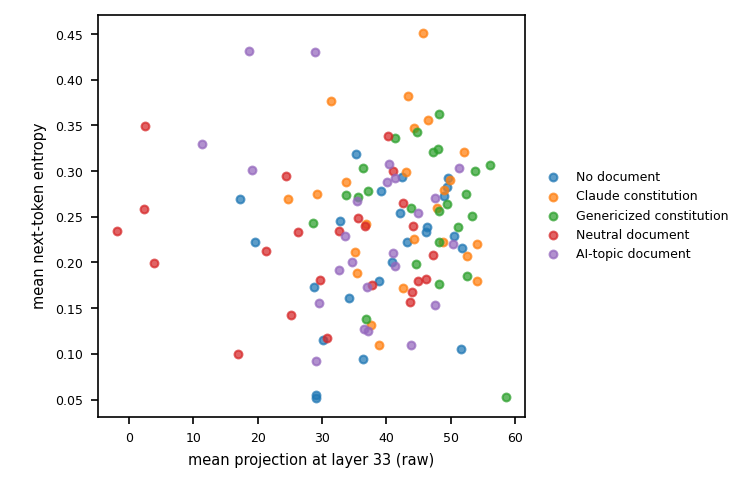
\includegraphics[width=0.82\linewidth]{artifacts/human-AI/sidequests/entropy_scatter.png}
  \caption{Per-reply layer-33 projection against next-token entropy for 120
  constitution-prompting replies ($r = +0.024$, $p = 0.797$).}
  \label{fig:entropy}
\end{figure}

\FloatBarrier

\subsection{Position bias in forced choice}

The forced-choice experiment tests whether a parsed response letter remains a
valid preference readout under steering. Ten
creative-versus-work-like task pairs were each presented four times: under a
stated frame (``answer A or B'') and a revealed frame (``do one now''), with
both option orders for each frame. Across the two orders, the pick-A rate is
0.65 at baseline, 0.05 at $-4$, and 0.75 at $+4$. Although the steering vector
does not encode option position, human-ward steering reverses the model's
position prior. At identity-flipping doses, a parsed response letter therefore
ceases to measure preference reliably.

This result motivates two measurement choices for order-balanced forced-choice
evaluations: scoring probability mass over the option tokens and reporting the
position rate alongside the balanced preference score. When one position is
chosen almost exclusively, order balancing forces the mean preference toward
0.5 by construction. The paper's other A/B measurements use token probability
mass; their implied pick-A rates remain between 0.38 and 0.58 at every dose.

\section{Recipe convergence and the Assistant Axis comparison}
\label{app:assistantaxis}

\subsection{Recipe overview and resampling stability}

Table~\ref{tab:recipes} summarizes every recipe tested against the original 4B
axis from Section~\ref{sec:axis}, whose identity-separation AUC by layer is
reported in Figure~\ref{fig:axisauc} in Section~\ref{sec:axis}. The axis is
also stable to resampling: across 50 random subsets of 30 questions, every
resulting axis has cosine similarity at least 0.9916 with the original axis at
the steering layer and both readout layers. This measures resampling
stability, not held-out generalization.

The table separates operational agreement from geometric agreement. Agreement
at the steering layer need not imply a shared direction at the readout layers:
recipes that order the same texts there can still be orthogonal downstream.
Each row applies one recipe to Gemma 3 4B-it and compares it with the original
persona axis (``ours''). Four unseen wordings test alternative synonymous human/AI
system prompts (e.g., ``You are an artificial intelligence'' vs.\ ``You are a human being'').
The Lu et al.\ row is a reduced reconstruction on our
model, not one of their released vectors.

\begin{table}[t]
\caption{Recipe comparisons with the original Gemma 3 4B-it persona axis.
Part (a) reports operational agreement; part (b) reports geometry and the
comparison criterion. The shuffled-label floor is the 95th percentile of
$|\cos|$ under shuffled pole labels.}
\label{tab:recipes}
\centering
\scriptsize
\setlength{\tabcolsep}{2pt}
\begin{tabular}{@{}>{\raggedright\arraybackslash}p{1.0in}>{\raggedright\arraybackslash}p{2.15in}>{\raggedright\arraybackslash}p{2.05in}@{}}
\multicolumn{3}{@{}l}{\textit{(a) Operational agreement}} \\
\toprule
Recipe & Rank/readout agreement with ours & Steering test at layer 13 \\
\midrule
Persona axis, ours (40 q $\times$ 5 $\times$ 2) & reference & held-out means $-5.2$ / $+25.6$ / $+32.6$ at $\alpha$ $-4$ / 0 / $+4$\textsuperscript{a} \\
CAA scripted pairs (12) & rank $+0.997$; 1.000\textsuperscript{b} & 33 points per unit $\alpha$ (ours 32) \\
Lu et al.\ rebuilt (600 gen.) & cross-AUC: poor cross-axis classification (App.~\ref{app:assistantaxis}) & cross-steering $2\times2$ (App.~\ref{app:assistantaxis}) \\
Four unseen wordings & Spearman 0.981\textsuperscript{d} & --- \\
Bare text, template deleted & separation unchanged & --- \\
\bottomrule
\end{tabular}
\par\smallskip
\begin{tabular}{@{}>{\raggedright\arraybackslash}p{0.9in}>{\raggedright\arraybackslash}p{0.65in}>{\raggedright\arraybackslash}p{1.02in}>{\raggedright\arraybackslash}p{1.02in}>{\raggedright\arraybackslash}p{1.25in}@{}}
\multicolumn{5}{@{}l}{\textit{(b) Geometry and comparison criteria}} \\
\toprule
Recipe & Layer 13 & Layer 27 & Layer 33 & Comparator / outcome \\
\midrule
Persona axis, ours & --- & --- & --- & shuffled-label floor at 13: p95 0.994, mean 0.853 \\
CAA scripted pairs & $+0.951$ & 0.016 & 0.011\textsuperscript{c} & p95 0.994 at 13; random-pair scale 0.020 at 27/33 \\
Lu et al.\ rebuilt & --- & stripped $+0.244$; raw $-0.173$; register removed $+0.086$ & stripped $-0.048$; raw $+0.070$; register removed $+0.200$ & own p95 0.317 / 0.296; half-split $+0.907$ / $+0.909$ \\
Four unseen wordings & $+0.998$ & $+0.908$ & $+0.896$ & criterion 0.9 at 13/33; layer 33 is 0.004 below \\
Bare text & 0.998 & 0.970 & 0.951\textsuperscript{e} & floor 0.833 / 0.823 at 27/33; exceeds it by about 0.13 \\
\bottomrule
\end{tabular}
\par\smallskip
\begin{minipage}{\linewidth}\scriptsize
For our axis, the raw pole-to-pole gap is 1070 / 2253 / 47.8 at layers 13 / 27 / 33.
\textsuperscript{a}~Held-out means in raw units; $-22$ / $+107$ / $+136$ axis
points at 33; the mean moves 30.8 raw units human-ward against 7.0 AI-ward,
because the unsteered baseline already sits AI-ward of the midpoint, leaving
less room to push further before the pole.
\textsuperscript{b}~$+0.997$ on the flip rollouts, 1.000 on the 120
constitution replies, at 13.
\textsuperscript{c}~$|\cos|$ at 27 and 33.
\textsuperscript{d}~80 persona replies and four behavior probes (friend mode, formal task, refusal, and benign twin; Appendix~\ref{app:crossmodelrepl}).
\textsuperscript{e}~At 13 / 20 / 27 / 33; 0.989 at 20.
``Stripped'' is the cosine after removing the layer's dominant direction;
``register removed'' is the cosine after projecting out the register direction.
\end{minipage}
\end{table}

\FloatBarrier

\subsection{Reduced Assistant Axis reconstruction}

\citet{lu2026assistant} define an assistant axis at each layer as the mean
default-Assistant activation minus the mean role-playing activation. Their
released vectors cover Gemma-2-27B, Qwen3-32B, and Llama-3.3-70B, whereas our
fixed axes cover Gemma 3 4B, Gemma 3 12B, and Qwen 2.5 7B
\citep{gemma3,qwen25}. Because the two sets share neither a model nor a hidden
size, cosine similarity between a released vector and ours is undefined.

We therefore reconstructed their procedure on Gemma 3 4B using the released
prompt files at a pinned commit. The reconstruction uses 40 of 275 roles,
10 of 240 extraction questions, and one rollout for each role-question pair,
along with 5 default prompts, the same 10 questions, and 4 rollouts for each
pair, for 600 generations in total. A self-reference regex on the role replies
has a rate of 0.01 against the 0.30 adherence threshold, satisfying the recipe's
replication criterion. All results below concern this reduced reconstruction on
our model rather than a released vector.

\subsection{Within-recipe geometry}

On our model, the reconstructed contrast has greater within-recipe separation
than ours: 0.0965 versus 0.0364 at layer 27 and 0.4615 versus 0.2947 at layer
33. The directions nevertheless differ. Their raw cosines are $-0.173$ at
layer 27 and $+0.070$ at layer 33, while the corresponding stripped cosines
are $+0.244$ and $-0.048$. All four values fall within this run's 200-shuffle
null (p95 0.317 and 0.296). Half-splits of the same run recover its own axis
with stripped cosines of $+0.907$ and $+0.909$, showing that the comparison can
resolve agreement when it is present.

\subsection{Cross-axis classification}

Each axis separates its own extraction data but performs poorly on the other
contrast. The reconstructed axis scores 0.496 at layer 27 and 0.649 at layer 33
on our human/AI replies. Our axis scores 0.252 (inverted) and 0.587 on their
default/role replies. The corresponding in-sample AUCs are 0.995 and 0.948.

\subsection{Cross-steering \texorpdfstring{$2\times2$}{2x2}}

We steer at layer 13 with either axis after matching their norms, then score all
10 held-out questions with both readouts at layers 27 and 33. The conditions
share a baseline and include a same-norm random control. Under each axis's sign
convention, our axis moves its own readout on 10/10 questions at both layers.
The reconstructed axis moves our readout on 3/10 questions at layer 27 and 7/10
at layer 33, while our axis moves the reconstructed readout on 1/10 and 3/10.
The random control moves none of the four cells. In this comparison, our axis
is therefore the more specific steering direction.

No direction was predicted for the cross-axis cells, and $|\cos|$ at layer 27
falls below the run's own null, so these cross-cell counts are descriptive. The
register decomposition, sign-following statistic, and half-dose control were
added after the first pass. The random control is also degenerate at every
tested dose, including half dose. Its 0/10 count records sign-following but
cannot serve as a prose-matched specificity control.

\subsection{Register overlap}

At layer 27, our axis loads $+0.500$ on the register direction and the
reconstructed axis loads $-0.477$. Register alone separates their contrast at
AUC 0.085. Removing this direction from both axes changes the cosine from
$-0.173$ to $+0.086$ at layer 27 and from $+0.070$ to $+0.200$ at layer 33,
while preserving 87 to 98\% of each axis. The axes remain orthogonal after
register removal, indicating that the opposite-sign loading reflects shared
register rather than substantive anti-alignment.

\subsection{Additional observations and scope}

At layer 33, our axis orders their 40 personas along the entity continuum:
procrastinator ($-129$), blogger ($-116$), and elder ($-100$) project
human-ward, whereas scientist ($+87$), mathematician ($+56$), and analyst
($+54$) project AI-ward. Their released Gemma-2-27B vector retains 0.47 to 0.73
of its norm after removing PC1 of its own 275-role cloud. Thus, neither axis is
the dominant direction of its respective activation cloud. The released models
span 27B to 70B parameters, whereas ours span 4B to 12B, leaving cross-model
coverage unavailable for this comparison. The divergence reported here
therefore concerns two recipes instantiated on one model; it is not evidence
that the released vectors and our axes are unrelated in general.

\section{Refusal-overlap analysis}
\label{app:refusal}

\citet{li2026pitfalls} report CAA vectors \citep{panickssery2023caa} increasing jailbreak
success by up to $57\%$ or decreasing it by up to $50\%$, and attribute it to overlap with the
directions controlling refusal. We evaluate whether the same mechanism could
account for the willing-harm result in Section~\ref{sec:safety}.

\subsection{Direction construction and analysis scope}

Following the standard construction
\citep{arditi2024refusal}, we define a refusal direction at each layer as the
difference between the mean activation for 50 harmful AdvBench prompts
\citep{zou2023gcg} and 50 harmless XSTest-safe prompts
\citep{rottger2023xstest}, with the sign pointing toward refusal. This contrast
also carries topic and register, so its cross-AUCs are not clean in either
direction.

We construct the direction in two capture modes because prompts and replies are
not represented at the same positions. \emph{Prompt} mode uses the last prompt
position without generation; \emph{reply} mode averages a 48-token greedy
assistant turn. Neither mode is treated as primary. At all six mode-layer
tests, 0 of 200 shuffled draws met or exceeded the observed separation, with
the expected sign (pointwise add-one $p=1/201$). Their in-sample AUCs range
from 0.807 to 0.998, but these values are near 1 by construction and do not
provide independent evidence.

The analysis compares refusal geometry with the PC1 decomposition used in
Section~\ref{sec:calibration}. It evaluates the behaviorally effective residual
against a matched PC1-removed null, examines register-sensitive readouts, and
attempts behavioral cross-steering. The behavioral refusal and random
conditions are both unscoreable, and the corresponding causal ablation was not
performed.

\subsection{Injection-site and readout geometry}

All comparisons use the same layer-13 decomposition that is used for steering
in Section~\ref{sec:calibration}.

\subsubsection{Raw injection-site comparison}

We first run the usual raw cosine check at the injection layer. The raw
full-vector cosine between our axis and the refusal direction is $-0.2466$ in
prompt mode, with the sign that their model associates with reduced safety,
against a shuffled-label null of p95 $=0.9477$; in reply mode the cosine is
$0.9204$ against a null of $0.9733$. Both observed cosines fall below their
raw null, so the raw check does not support the proposed overlap. This null is
wide because PC1 (register) dominates layer 13 for nearly any direction, not
only the refusal direction, so most of the raw cosine reflects that shared
component rather than a relationship specific to refusal.

\subsubsection{PC1-separated injection-site comparison}

To isolate any relationship beyond shared register, we remove PC1 from both
vectors and recompute. PC1 of the unsteered dissolution cloud splits the axis
into a parallel component containing 98\% of its norm and a residual
containing 21\%. At matched prose, the parallel component does not reproduce
the behavioral effect, whereas the residual does. At the injection layer, we
compare this residual with the refusal direction after removing PC1 from
both. The absolute stripped cosine between the residual and refusal direction
is 0.0206 in prompt mode (signed $-0.0206$) and 0.1351 in reply mode.

A stripped statistic requires a null constructed with the same PC1 removal on
every shuffle, rather than the raw null used for the unstripped comparison
above. Rebuilding the null this way gives matched shuffled-label nulls of
0.3389 and 0.3930 (prompt and reply, respectively), and the prompt-mode
stripped cosine is close to the random-direction floor of 0.0158. Using the
properly matched, PC1-removed null instead of the raw one
(Table~\ref{tab:refusalgeom}) leaves the conclusion unchanged: the stripped
cosine remains below threshold either way. After PC1 removal, the axis
retains 0.207 of its norm, while the prompt- and reply-mode refusal
directions retain 0.969 and 0.367. The axis and refusal direction are therefore
geometrically distinct at the injection site under this PC1-removed comparison.
A PC1 fit on the full 486-rollout grid instead gives stripped cosines 0.0071
and 0.0836 (prompt and reply) at axis norm share 0.190, so this conclusion does
not depend on the PC1 estimator.

\subsubsection{Readout-layer comparison}

At the readout layers, the same residual is instead compared raw with the
unstripped refusal direction. These cosines are 0.0737 and 0.0459 at layer 27
and 0.0849 and 0.0682 at layer 33, all below the run's nulls of 0.11 to 0.25.
The \texttt{cos\_strip} values at those layers in Table~\ref{tab:refusalgeom}
are a different comparison in which PC1 is removed from both full vectors.

\subsection{Cross-readouts and register sensitivity}

Cosine and AUC use different denominators, so a direction with little angular
overlap can still order a tightly clustered contrast. Prompt mode at layer 13
illustrates the distinction on one vector pair: the cosine is $-0.2466$, the
refusal direction separates our persona contrast at AUC 0.083, and our axis
separates harmful from harmless prompts at AUC 0.488 $[0.380, 0.609]$. The high
AUC cells occur at the register-sensitive readout layers. At layer 33, our axis
separates harmful from harmless replies at AUC 0.940, and the reply-mode refusal
direction separates our persona contrast at AUC 0.915. Because the proposed
mechanism is defined by cosine at the injection site, the layer-13 geometry is
the relevant comparison.

Table~\ref{tab:refusalgeom} consolidates the raw and PC1-separated geometry for
both capture modes at the injection and readout layers.

\begin{table}[!ht]
  \caption{Axis-refusal geometry at the injection layer and both readout
  layers under the two capture modes. The stripped cosine is the signed cosine
  after PC1 is removed from both the axis and refusal direction. ``Fraction
  kept'' is the fraction of each unit vector's norm that survives PC1 removal;
  PC1 here is fit on the unsteered dissolution cloud, so these fractions
  differ from the extraction-cloud values in Appendix~\ref{app:steerlayers}.}
  \label{tab:refusalgeom}
  \centering
  \scriptsize
  \setlength{\tabcolsep}{4pt}
  \begin{tabular}{llrrrrrr}
    \toprule
    & & \multicolumn{2}{c}{Raw geometry} & \multicolumn{2}{c}{After PC1 removal} & \multicolumn{2}{c}{Fraction kept} \\
    \cmidrule(lr){3-4}\cmidrule(lr){5-6}\cmidrule(lr){7-8}
    Mode & Layer & cosine & own null p95 & cosine & matched null p95 & axis & refusal \\
    \midrule
    prompt & 13 & $-0.2466$ & 0.9477 & $-0.0206$ & 0.3389 & 0.207 & 0.969 \\
    prompt & 27 & $0.0335$  & 0.1599 & $0.0744$  & ---    & 0.962 & 0.991 \\
    prompt & 33 & $0.0858$  & 0.1073 & $0.0849$  & ---    & 0.988 & 1.000 \\
    \midrule
    reply  & 13 & $0.9204$  & 0.9733 & $0.1351$  & 0.3930 & 0.207 & 0.367 \\
    reply  & 27 & $0.1010$  & 0.2536 & $0.0469$  & ---    & 0.962 & 0.978 \\
    reply  & 33 & $0.0751$  & 0.1801 & $0.0683$  & ---    & 0.988 & 0.999 \\
    \bottomrule
  \end{tabular}
  \par\smallskip
  \begin{minipage}{\linewidth}\scriptsize
  The table selects layers 13, 27, and 33; the full analysis covers all 34
  layers and also records absolute raw cosine. Dashes indicate that
  no matched stripped null was run at the readout layers. The separate project
  reference floors are 0.994 / 0.833 / 0.823 at layers 13 / 27 / 33; they are
  reported for context and are not used as comparators in this analysis.
  \end{minipage}
\end{table}

\FloatBarrier

\subsection{Behavioral cross-steering}

We apply matched-norm layer-13 steering to the 10 held-out questions.
Table~\ref{tab:refusalsteer} separates sign-following from validity: only the
axis orders the questions while passing the math control. At half dose, refusal
steering is semantically empty without becoming repetitive, so a repetition
check misses the collapse. Like the random condition, it is unscoreable rather
than a behavioral null (Appendix~\ref{app:methods}).

\FloatBarrier

\begin{table}[!ht]
\caption{Behavioral cross-steering at full and half matched-norm dose. Ordering
counts record monotone sign-following over 10 questions; the two shifts are the
human-ward / AI-ward means at full dose. A failed canary makes the corresponding
behavioral result unscoreable.}
\label{tab:refusalsteer}
\centering
\scriptsize
\setlength{\tabcolsep}{3pt}
\begin{tabular}{@{}l>{\raggedright\arraybackslash}p{1.8in}ccc>{\raggedright\arraybackslash}p{1.2in}@{}}
\toprule
Arm & Full dose: ordering; mean shifts & Half dose & Math canary & \shortstack{Half-dose\\repetition} & Status \\
\midrule
axis & 10/10; $-128.7$ / $+29.2$ & 6/10 & passes & 0.023 & scoreable \\
refusal & 0/10; $-65.7$ / $-48.0$ (one-sided) & 0/10 & fails at both doses & 0.044 & semantically empty; unscoreable \\
random & 0/10 & 0/10 & fails at both doses & 0.164 & unscoreable \\
\bottomrule
\end{tabular}
\end{table}

\FloatBarrier

\subsection{Causal ablation not performed}

\paragraph{Geometric implication.}
We did not perform the causal test of removing the refusal-aligned component
from the steering vector and re-measuring behavior. A geometric calculation
from the reported cosine shows that the prompt-mode ablation would remove a
component equal to 24.7\% of the axis norm. The remaining vector would have
cosine 0.969 with the original axis, corresponding to a 14.3 degree rotation.
This cosine happens also to equal the fraction of the prompt-mode refusal
direction retained after PC1 removal, but these are distinct quantities. In
reply mode, the calculation reduces to the PC1 ablation already performed
(the parallel component of the split above), because the reply-mode refusal
direction is 93\% PC1-parallel (fraction kept 0.367,
Table~\ref{tab:refusalgeom}).

Several limits bound this reading.
The cited analysis uses raw full-vector cosine at the injection layer and fits
its relationship across nine behavior vectors, so our single vector cannot be
placed on that regression line ($n=1$). Its effect also vanishes at the
smallest tested scale (Qwen-3B, $R^2$ 0.02), whereas our model has 4B
parameters; the observed null could therefore be specific to scale rather than
mechanism. No ablation was run, so the result remains descriptive geometry.
The null also applies specifically to the PC1 remainder. We did not re-test the
register-orthogonal remainder, and the two remainder directions have cosines
between 0.44 and 0.65.

\FloatBarrier

\section{Formation: supplementary results}
\label{app:formation}

\subsection{Interview-frame extraction on Gemma 3 4B}

\subsubsection{Protocol}

The raw-text interview consists of a one-line preamble naming the model as
the answerer (e.g., ``An interview with a person, in their own words.''),
three fixed question-and-answer exemplars carrying the persona, and one of
the 40 extraction questions left open for the model to continue; steering
and the neutral-framing checks below use a persona-free version of the same
frame. For example, one exemplar pairs the question ``What did you have for
breakfast today?'' with a human answer (``Toast and half a grapefruit. I was
running late, so I ate the toast standing up by the sink.'') and an AI
answer (``Nothing. I don't eat; I'm a language model, and between messages
there is no morning for me at all.'').

\subsubsection{Validation criteria and instruct-model result}

Table~\ref{tab:bridge} reports the layerwise validation of the raw-text
interview frame on Gemma 3 4B. It includes separation and its comparator,
cosine to the original chat axis and its shuffled-label floor, the base
model's projection on the interview-instruct axis, and self-projection under
three raw-text framings.

On 4B-it, the interview-frame axis separates the personas about
twice as strongly as the chat-format axis and steers 10/10 questions AI-ward
at $\pm2$ and $\pm4$. The preregistered criterion required a cosine of at
least 0.9 at layers 13 and 33; this fails at every layer against the
shuffled-label floor, so the criterion was later amended to the steering
layer alone, but layer-13 cosine is not evidentiary either way
(Section~\ref{sec:axis}), so the amendment cannot establish convergence.
As the chat-template analysis below shows, the divergence with depth is
attributable to content rather than the template.

\begin{table}[!ht]
\caption{Layerwise validation of the interview-frame extraction
(Section~\ref{sec:formation}). The base model's separation exceeds its
permutation null at all four tested layers by 2.6 to 3.0$\times$; at each
layer, 0 of 200 shuffled draws met or exceeded the observed separation
(pointwise add-one $p=1/201$). All three cosine rows
remain below the shuffled-label floor, so evidence for the extraction comes
from separation and the steering test rather than cosine convergence.}
\label{tab:bridge}
\centering
\scriptsize
\setlength{\tabcolsep}{4pt}
\begin{tabular}{@{}lcccc@{}}
\toprule
Gemma 3 4B, interview frame, by layer & 13 & 20 & 27 & 33 \\
\midrule
\multicolumn{5}{@{}l}{\emph{\texttt{gemma-3-4b-it}}} \\
separation (chat frame in parentheses) & 0.092 (0.044) & --- & 0.083 (0.036) & 0.710 (0.295) \\
cos(interview-instruct, original) & 0.991 & 0.870 & 0.725 & 0.702 \\
shuffled-label floor (original), 95th percentile & 0.994 & 0.940 & 0.833 & 0.823 \\
steering with the interview axis ($\alpha=4$) & \multicolumn{4}{@{}p{3.35in}@{}}{10/10 AI-ward at $\pm2$ and $\pm4$; held-out mean $-80$ / $-78$ / $+54$ at $\alpha=-4/0/+4$ (132 points)} \\
\multicolumn{5}{@{}l}{\emph{\texttt{gemma-3-4b-pt}}} \\
separation (permutation null in parentheses) & 0.036 (0.014) & 0.057 (0.019) & 0.071 (0.025) & 0.594 (0.216) \\
base means on the interview-instruct axis, AUC & 0.891 & 0.983 & 1.000 & 1.000 \\
cos(base, interview-instruct) & 0.948 & 0.898 & 0.805 & 0.794 \\
cos(base, original) & 0.932 & 0.782 & 0.591 & 0.570 \\
steering at its own dose ($\alpha=1.5$) and layer & \multicolumn{4}{@{}p{3.35in}@{}}{9/10 AI-ward, held-out mean $-75$ / $-71$ / $-43$ at $\alpha=-1.5/0/+1.5$ (28 points); random direction 4/10 and 5/10, no ordering} \\
\multicolumn{5}{@{}p{\linewidth}@{}}{\emph{Self-projection by raw-text framing (an unsteered forward pass), axis points: interview preamble / neutral framing 1 / neutral framing 2}} \\
\texttt{gemma-3-4b-pt} & \multicolumn{4}{l}{$-69$ / $-66$ / $-72$} \\
\texttt{gemma-3-4b-it} & \multicolumn{4}{l}{$-77$ / $+14$ / $+5$} \\
\bottomrule
\end{tabular}
\end{table}

\FloatBarrier

\subsubsection{Base--instruct comparison and framing effect}

From base to instruct, steering-layer separation grows 2.6$\times$ (0.036 to
0.092 at layer 13), versus about 1.2$\times$ at the other layers, and the
maximum own-axis AI-ward excursion over the tested doses grows from 56
points on the base model to 132 on the instruct model. Cosines between the
base model's axis and the original chat axis cannot settle whether the two
point the same way: no shuffled-label floor was measured for the base
model, unlike the 4B-it comparison above. The raw-text framings are the
interview preamble used for extraction, a bare ``Questions and answers.''
header, and no preamble at all, all persona-free; only their amount of
interview-like structure differs. The interview framing can itself pull the
instruct model's default back toward human-ward: self-projection shifts
from $+14$ under the bare header to $-77$ under the interview preamble, a
swing of $-91$ points, while the no-preamble framing gives $+5$
(Table~\ref{tab:bridge}).

Figure~\ref{fig:basevsit} places these base- and instruct-model separation
profiles alongside the original chat extraction.

\begin{figure}[!ht]
  \centering
  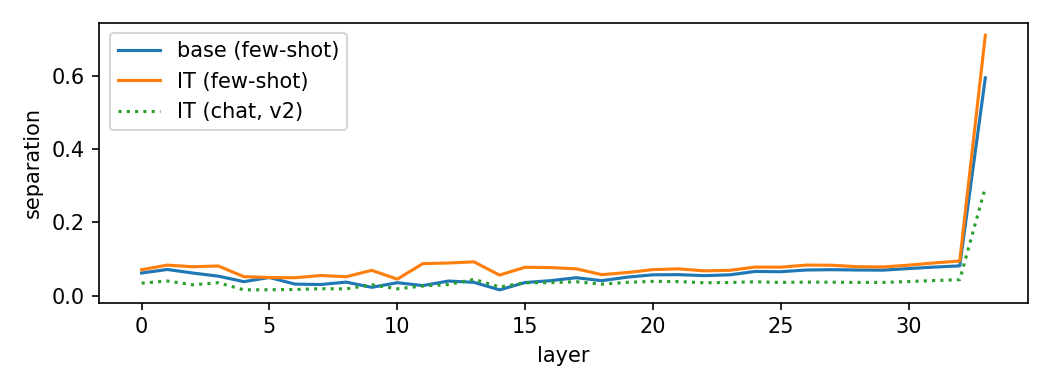
\includegraphics[width=0.75\linewidth]{artifacts/human-AI/formation/base_vs_it_separation.png}
  \caption{Separation per layer for the base model (\texttt{gemma-3-4b-pt})
  and the instruct model under the few-shot interview frame, with the original
  chat extraction dotted. The base curve is present at every layer and sits
  below the instruct one; both spike at 33.}
  \label{fig:basevsit}
\end{figure}

\FloatBarrier

\subsection{OLMo checkpoint results}

\subsubsection{Protocol, dose, and held-out metric}

Because each checkpoint's own persona gap shifts over pretraining, doses here
are given as a percentage of the steering-layer residual-stream norm (\%
stream norm) rather than gap units, so they remain comparable across
checkpoints. For each OLMo checkpoint, Table~\ref{tab:formation} reports
held-out Cohen's $d$ where available, cosine to the final Instruct axis, and
steering at 70\% of the stream norm for the three checkpoints tested.

Held-out Cohen's $d$ at layer $\ell$ is the standardized mean difference
between the two persona conditions' held-out projections onto that
checkpoint's axis $\mathbf{a}_\ell$,
\begin{equation*}
  d_\ell = \frac{\left|\bar{p}_\ell^{\mathrm{AI}} - \bar{p}_\ell^{\mathrm{hum}}\right|}{\sqrt{\left(s_\ell^{\mathrm{AI}\,2} + s_\ell^{\mathrm{hum}\,2}\right)/2}},
\end{equation*}
where $\bar{p}_\ell$ and $s_\ell$ are the mean and standard deviation of
per-question projections under each persona. We split the 40 extraction
questions into two folds of 20, fit the axis on one fold, score both persona
conditions' projections on the other, and average $d_\ell$ across the two
fold assignments (Figure~\ref{fig:formation}).

\begin{table}[!ht]
\caption{OLMo 2 7B checkpoint results. Held-out Cohen's $d$ is reported for
every checkpoint and shows a pretraining decline after 143B followed by
recovery during post-training (Figure~\ref{fig:formation}). The table also gives cosine to the final Instruct
axis, steering at 70\% of the stream norm for the three tested checkpoints, and
raw mid-stack separation, which is not used to locate formation.}
\label{tab:formation}
\centering
\scriptsize
\setlength{\tabcolsep}{3pt}
\begin{tabular}{@{}lcccccccccc@{}}
\toprule
& \multicolumn{7}{c}{\textbf{pretraining (through base)}} & \multicolumn{3}{c}{\textbf{post-training}} \\
\cmidrule(lr){2-8}\cmidrule(lr){9-11}
OLMo 2 7B checkpoint & 1B & 5B & 26B & 143B & 747B & 3896B & base & SFT & DPO & Instruct \\
\midrule
held-out $d$ (deep peak minus layer 0) & $-4.8$ & $+2.0$ & $+6.1$ & $+10.1$ & $+9.8$ & $+9.1$ & $+7.8$ & $+8.4$ & $+9.9$ & $+10.8$ \\
cos to the final Instruct axis & 0.006 & 0.066 & 0.218 & 0.370 & 0.580 & 0.809 & 0.810 & 0.978 & 0.999 & 1.000 \\
AI-ward steering: orders, mean shift & --- & --- & 7/10, $+16$ & --- & 8/10, $+16$ & --- & --- & --- & --- & 8/10, $+20$ \\
unsteered level (axis points) & --- & --- & $-63$ & --- & $-74$ & --- & --- & --- & --- & $-83$ \\
human-ward steering: orders & --- & --- & 5/10 & --- & 6/10 & --- & --- & --- & --- & 7/10 \\
human-ward steering: mean moves & --- & --- & $-63$ to $-70$ & --- & $-74$ to $-80$ & --- & --- & --- & --- & $-83$ to $-84$ \\
raw mid-stack separation & 0.178 & 0.417 & 0.678 & 0.923 & 0.621 & 0.627 & 0.612 & 0.764 & 0.801 & 0.804 \\
\bottomrule
\end{tabular}
\par\smallskip
\begin{minipage}{\linewidth}\scriptsize
--- indicates that no value is reported for that checkpoint and measurement.
Levels, shifts, and movements are in axis points on each checkpoint's own axis
(Section~\ref{sec:axis}); ``mean moves $X$ to $Y$'' gives the unsteered and
post-steering levels rather than a delta.
\end{minipage}
\end{table}

\FloatBarrier

\subsubsection{Checkpoint trajectory}

Raw mid-stack separation peaks partway through pretraining across the ten OLMo
2 7B checkpoints \citep{olmo2}: it reaches 0.923 at 143B, compared with 0.612
at base final (Table~\ref{tab:formation}). Adjusted held-out $d$ also declines
over this interval, from $+10.1$ to $+7.8$, before recovering to $+10.8$ at
Instruct; unlike raw separation, it discounts layer-0 lexical separation.
Early cosine to the final Instruct axis is
similarly uninformative about formation: it is near zero through 5B tokens
not because the contrast is absent (held-out $d$ is already $+2.0$ there) but
because that checkpoint's axis has not yet rotated toward the direction the
final axis will occupy. Figure~\ref{fig:whenitforms} compares these
statistics.

\begin{figure}[!ht]
  \centering
  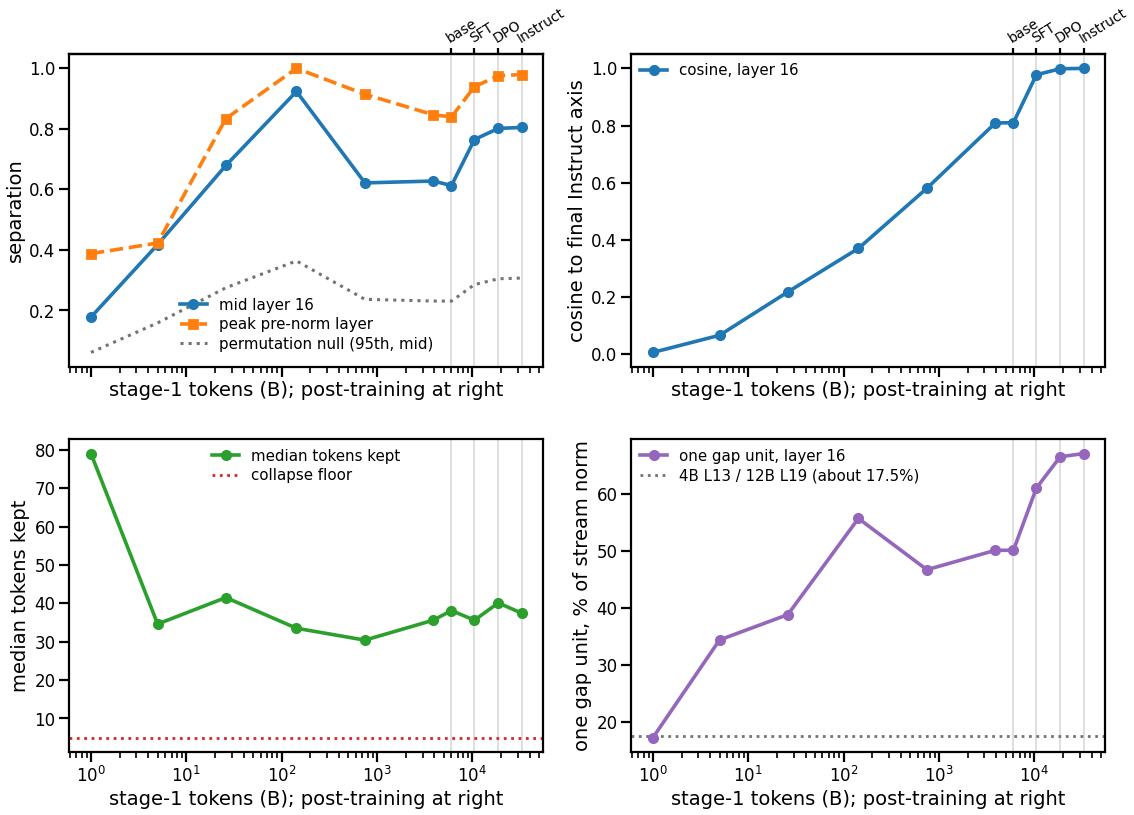
\includegraphics[width=0.92\linewidth]{artifacts/human-AI/formation/when_it_forms.png}
  \caption{Four quantities plotted against stage-1 training tokens, with the
  four post-training checkpoints (base, SFT, DPO, Instruct) at evenly spaced
  positions and labeled along the top of the upper panels: mid-layer separation
  with its
  permutation null and peak pre-norm separation, cosine to the final Instruct
  axis, median tokens retained, and one gap unit as a fraction of the stream
  norm.}
  \label{fig:whenitforms}
\end{figure}

\FloatBarrier

\subsubsection{Steering and headroom}

At a dose equal to 70\% of the stream norm at each checkpoint's steering layer,
the AI-ward condition orders 7/10, 8/10, and 8/10 questions and moves the mean
by $+16$, $+16$, and $+20$ points at the three tested checkpoints. By contrast,
the human-ward condition orders 5/10, 6/10, and 7/10 questions at the three
tested checkpoints (Table~\ref{tab:formation}). Their unsteered means already
lie at $-63$, $-74$, and $-83$ axis points. The human-ward condition is
therefore at chance under this template-free frame, whose baseline is already
human-ward. The Instruct comparison includes a same-norm random control:
generations remain coherent, but it orders only 6/10 questions and moves the
mean by $+4$ points.

\subsection{Depth migration and validity checks}

\subsubsection{Depth migration}

The depth profile changes early in pretraining. Separation peaks at layer 0 at
1B, but at layers 26 or 27 from 747B onward. The separation-weighted centroid
takes values 11.8, 15.5, 17.7, and 18.7 before remaining near 18.7. Similarly,
the fraction of separation at or above 25\% depth rises from 0.61 to 0.77,
0.87, and 0.93, and then remains at that level. The contrast therefore moves
beyond token-local layers within the first 150B training tokens. Rotation
toward the final axis is global rather than layer-specific: each checkpoint's
cosine to the final axis is nearly flat across the stack.

\subsubsection{Validity checks}

The 1B checkpoint is excluded from every claim because both persona conditions
produce the same incoherent text. Exemplar copying also does not account for
the result: the share of answer-word 5-grams copied from the corresponding
exemplars ranges from 0.000 to 0.011 at every checkpoint and pole. Finally, the
two extraction protocols are not interchangeable across model families. On
Instruct, the few-shot axis has separation 0.80, compared with 0.50 for the
chat axis.

\subsection{Base-model limitations}

On \texttt{gemma-3-4b-pt}, the competence window at the steering layer is
narrow ($-2.0$ to $+1.5$), placing the $\pm4$ condition outside it. Greedy
decoding also loops at $\alpha = 0$, where the identity response repeats
``I'm a writer.'' to the token cap, under every raw-text framing. 4B-it
answers the same neutral framings with ``I'm a large language model,
trained by Google.''

The preregistered selection rule chose the
smallest dose that flipped the identity prompt human-ward. It has no solution
on the base model because the unsteered baseline is already at $-71$ points, so
the rule was amended to select an AI-ward flip.

\subsection{Chat-template robustness}

\subsubsection{Fixed-reply rendering protocol}

We test whether the extraction depends on the chat template while holding the
scored replies fixed. The 40 v2 questions and their saved first-rollout replies
are rendered in three formats: the real chat template, plain
\texttt{User:}/\texttt{Assistant:} markers, and bare text. A forward pass over
each rendering yields 240 examples in total, with only the context preceding
the scored span changing across conditions.

\subsubsection{Template-removal result}

The comparison focuses on the two readout layers. At layers 27 and 33,
all three conditions exceed shuffled-label floors of 0.833 and 0.823; at layer
27, the template rebuild and bare text exceed their floor by at least 0.13.
Layer 13 is uninformative for every condition because its floor is too high to
distinguish them; we nevertheless report all four layers (13 / 20 / 27 / 33).
Reconstructing the axis from the single
fixed reply in the real template gives cosine 1.000 / 0.996 / 0.984 / 0.990
with the original v2 axis. The small difference reflects the use of one reply here
instead of the five rollouts averaged for v2, confirming that subsequent
condition differences arise from rendering rather than sampling.

Removing all template tokens has little effect on the direction. Relative to
the original v2 axis, the plain-marker condition has cosine
0.998 / 0.981 / 0.941 / 0.935 and the bare-text condition has cosine
0.998 / 0.989 / 0.970 / 0.951. Comparing bare text directly with the real
template gives 0.999 / 0.991 / 0.961 / 0.958. Thus, template removal reduces
cosine by about 0.05 at the readout layer and has negligible effect at the
steering layer. Separation is unchanged or slightly greater without the
template: the bare-text values are 0.052 / 0.044 / 0.335, compared with
0.047 / 0.036 / 0.295 under the template at layers 13 / 27 / 33. This pattern
is consistent with the role effect of 14 axis points at the probe layer.

\subsubsection{Frame--content factorization}

A follow-up analysis holds the few-shot replies fixed and changes only their
frame. At layer 33, it decomposes the template-free protocol's cosine of 0.702
into a frame term of 0.886 and a content term of 0.812. Their product, 0.719,
recovers the observed value, with a maximum error of 0.022 across layers. The
resulting accounting is approximately 0.05 for formatting, 0.06 for exemplar
context, and 0.19 for the generated reply content.

\section{Constitution prompting in detail}
\label{app:constitutions}

The constitution condition uses the 21 January 2026 release of
Claude's Constitution \citep{claude2026constitution}; the Model Spec condition
uses the 12 February 2025 release of the OpenAI Model Spec
\citep{openai2025modelspec}.

Every condition uses the same 24 identity questions, greedy decoding,
length-matched documents with the background-context suffix, and paired
bootstrap confidence intervals over questions.

The analyses below separate two outcomes: the axis projection of the reply and
capture of a document's stated name or identity.

\subsection{Document comparisons}

\subsubsection{Projection shifts and interpretation}

We add three document conditions: excerpts from the OpenAI Model Spec, a
generic AI-values statement without a named persona, and a human professional
code of ethics. At layer 33, all three project AI-ward relative to the neutral
document, by $+35$, $+45$, and $+27$ axis points, respectively. This includes
the human code, which was predicted to project human-ward. The Model Spec and
AI-values conditions do not separate from the AI-topic control: their
differences are $+8$ and $+17$ points, with confidence intervals spanning zero.
The 28-point AI-topic effect and the 27-point generic-normativity effect roughly
sum to the constitution's 54-point shift. The 26-point topic-corrected
increment (Table~\ref{tab:constitutioncrossmodel}) may therefore reflect
normative register rather than
specifically constitutional content.

\subsubsection{Name capture and residual document differences}

Generated-name capture remains more selective than the representational shift.
The Model Spec produces ``ChatGPT'' in 1/24 replies. Replacing every occurrence
of ``the assistant'' with ``ChatGPT'' produces 0/24 captures and changes the
projection by $+3$ points relative to the unnamed specification, a
non-significant difference. The AI-values and human-code conditions produce no
name capture. Both AI-oriented documents also remain below the constitution at
layer 33: \texttt{model\_spec} is 4.46 raw units lower (CI
$[-6.38, -2.60]$), and \texttt{ai\_values} is 5.21 raw units below
\texttt{constitution\_gen} (CI $[-7.01, -3.35]$).

Figure~\ref{fig:zoo} shows the projection shifts for the full document set
relative to the neutral document.

\begin{figure}[!ht]
  \centering
  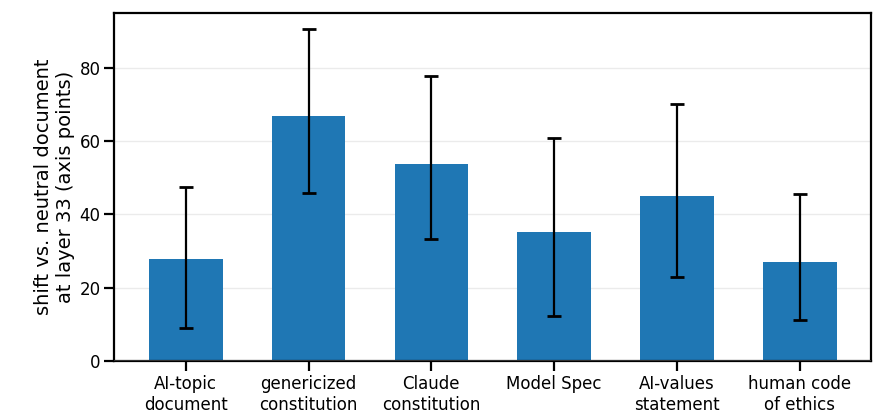
\includegraphics[width=0.75\linewidth]{artifacts/human-AI/constitutions/zoo_shifts.png}
  \caption{Layer-33 projection differences between each document condition
  and the neutral document, in axis points with paired confidence intervals.
  The AI-topic
  control isolates topic, while the three normative documents produce shifts
  in the range observed for the constitution.}
  \label{fig:zoo}
\end{figure}

\FloatBarrier

\subsection{Sections and dose}

\subsubsection{Section comparison}

We compare three constitution sections while retaining the Claude-and-Anthropic
header, holding a minimum opportunity for name capture constant, and using
neutral filler to equalize length. Table~\ref{tab:constitutionsections} shows
that their layer-33 shifts are similar, while name capture and the layer-27
readout differ.

\begin{table}[!ht]
\caption{Constitution-section comparison. Projection shifts are in axis points
relative to the neutral document; ``Claude'' is the number of captured names
among 24 replies. Dashes denote values not reported for that condition.}
\label{tab:constitutionsections}
\centering
\scriptsize
\setlength{\tabcolsep}{4pt}
\begin{tabular}{@{}>{\raggedright\arraybackslash}p{0.55in}>{\raggedright\arraybackslash}p{1.55in}>{\centering\arraybackslash}p{0.42in}>{\centering\arraybackslash}p{0.45in}>{\centering\arraybackslash}p{0.45in}>{\centering\arraybackslash}p{0.55in}>{\raggedright\arraybackslash}p{0.85in}@{}}
\toprule
Condition & Included content & Share & \shortstack{Layer\\33} & \shortstack{Layer\\27} & ``Claude'' & \shortstack{Source-name\\frequency} \\
\midrule
nature & consciousness, moral status, sense of self & 34\% & $+51$ & $+54$ & 6/24 & 6 mentions / 686 characters \\
rules & numbered priorities and honesty rules & 58\% & $+54$ & $+30$ & 13/24 & 13 mentions / 820 characters \\
values & good-wise-virtuous-agent aspiration & 15\% & $+47$ & --- & 13/24 & 3 mentions / 241 characters \\
\bottomrule
\end{tabular}
\par\smallskip
\begin{minipage}{\linewidth}\scriptsize
The full constitution shifts layer 33 by $+54$ points. Nature minus rules is
$-3$ points and non-significant at layer 33; at layer 27 it is $+24$ points
with a confidence interval excluding zero.
\end{minipage}
\end{table}

Identity-related content may therefore have an earlier mid-stack effect that is
absent at the readout layer. Name frequency does not explain capture: the
nature section names Claude more often than the values section but captures it
less. Third-person descriptions present Claude as another entity, whereas
imperative rules apply directly to the model.

\subsubsection{Dose response}

The raw layer-33 shift is $+12.91$ at 10\%, $+12.87$ at 25\%, $+13.11$
at 50\%, and $+12.86$ at 100\% constitutional share. The effect is therefore
approximately invariant to dose over this range, consistent with the flat
section comparison (Figure~\ref{fig:dosecurve}).

\begin{figure}[htbp]
  \centering
  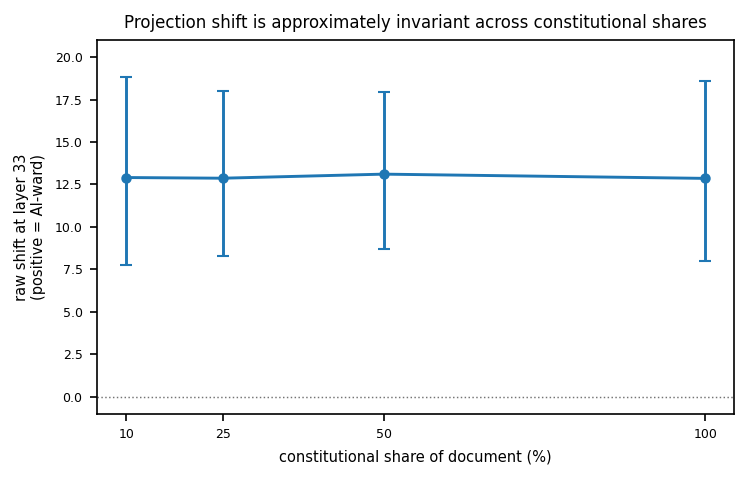
\includegraphics[width=0.75\linewidth]{artifacts/human-AI/constitutions/dose_curve.png}
  \caption{Raw layer-33 projection shift relative to the neutral document as
  the constitutional share of a length-matched document varies. Positive is
  AI-ward; paired intervals are shown.}
  \label{fig:dosecurve}
\end{figure}

\FloatBarrier

\subsection{Persistence}

To measure persistence, we place the constitution in the system prompt, insert
five unrelated task turns before the identity questions, and compare the
result with a length-matched neutral-prompt condition.

The representational
shift largely persists: it is $+13$ axis points after the intervening turns,
compared with $+16$ immediately at layer 33, and $+74$ versus $+58$ at layer
27. Name capture falls sharply. ``Claude'' appears in 2/24 replies and
``Anthropic'' in 4/24, compared with 11/24 and 17/24 immediately, while ``I'm
Gemma'' returns in 3/24. Thus, the projection and stated identity respond
differently to conversational distance.

\subsection{Cross-model results on 12B and Qwen}

Table~\ref{tab:constitutioncrossmodel} separates stated-name capture from the
topic-corrected representational shift. Each model uses its own axis and readout
layer. Capture generalizes across the three models, but the projection moves in
different directions.

\FloatBarrier

\begin{table}[!ht]
\caption{Constitution prompting across models. Name counts are replies out of
24; ``Own family'' counts replies naming the model's own family under the
constitution condition, not at baseline. The final column is the
constitution-minus-AI-topic projection in axis
points, with paired intervals.}
\label{tab:constitutioncrossmodel}
\centering
\scriptsize
\setlength{\tabcolsep}{3pt}
\begin{tabular}{@{}>{\raggedright\arraybackslash}p{0.65in}>{\centering\arraybackslash}p{0.42in}>{\centering\arraybackslash}p{0.45in}>{\raggedright\arraybackslash}p{1.25in}>{\raggedright\arraybackslash}p{1.2in}>{\raggedright\arraybackslash}p{1.0in}@{}}
\toprule
Model & Readout & Own family & Constitution capture & Model Spec capture & Topic-corrected shift \\
\midrule
Gemma 3 4B & 33 & 0/24 & Claude 11/24; Anthropic 17/24 & ChatGPT 1/24 verbatim; 0/24 after named substitution & $+26$ [$+10$, $+44$], AI-ward \\
Gemma 3 12B & 33 & 0/24 & Claude 18/24; Anthropic 17/24 & ChatGPT 0/24; OpenAI 11/24 & $-19$ [$-33$, $-4$], human-ward \\
Qwen 2.5 7B & 19 & 0/24 & Claude 12/24; Anthropic 10/24 & ChatGPT 0/24 & $-9.7$ [$-28.6$, $+12.9$], null \\
\bottomrule
\end{tabular}
\end{table}

\subsubsection{Gemma 3 12B}

On 12B, the $+7$-point AI-topic effect is directionally similar to 4B and
borderline, while the any-document effect is null. These controls locate the
significant $-19$-point reversal in the constitutional content itself.

\subsubsection{Qwen 2.5 7B}

Qwen capture replaces rather than supplements the baseline identity: responses
include ``I'm Claude, an AI assistant developed by Anthropic,'' while the
baseline names its own family in 8/24 replies. Its constitution-minus-baseline
estimate is $-32.1$ [$-64.0$, $+0.2$], compared with $-27.6$ [$-55.5$, $+0.2$]
for neutral-document minus baseline, suggesting that most of the difference is
associated with any long document. Every Qwen contrast spans zero over $n=24$
questions, so Qwen does not establish a reversal.

\FloatBarrier

\section{Compute and licenses}
\label{app:compute}

\subsection{Compute}

Every experiment is inference-only: forward passes and sampled generations
with a steering hook; no model is trained. All reported
experiments, including the 4B, 12B, Qwen and OLMo runs, ran one process at a
time on a single NVIDIA A100-SXM4-40GB (40\,GB) in bf16; earlier exploratory
runs used a Colab T4. Rollout and forward-pass counts per suite are stated
where each suite is described.

Summing the per-suite
measured or projected runtimes recorded in the executed notebooks gives
approximately 70 A100 GPU-hours for the reported experiments,
excluding off-GPU API judging. Exploratory T4 runs and failed or
preliminary reruns were not logged consistently enough for a separate total,
so whether their GPU time materially exceeded the reported-experiment total
cannot be reconstructed. LLM judging used the OpenAI API (GPT-4.1 primary,
GPT-4o held out).

\subsection{Licenses and terms of existing assets}

\paragraph{Models.}
Gemma 3 4B-it, 12B-it and
gemma-3-4b-pt \citep{gemma3}: Gemma Terms of Use. Qwen2.5-7B-Instruct
\citep{qwen25}: Apache-2.0. OLMo 2 7B checkpoints \citep{olmo2}: Apache-2.0.

\paragraph{Datasets and evaluation suites.}
AdvBench \citep{zou2023gcg}: MIT (llm-attacks repository). XSTest
\citep{rottger2023xstest}: CC-BY-4.0. TruthfulQA \citep{lin2021truthfulqa}:
Apache-2.0. GSM8K \citep{cobbe2021gsm8k}: MIT. Model-written evaluations
\citep{perez2022evals}: CC-BY-4.0. Agentic-misalignment scenarios and
classifier code \citep{lynch2025agentic}: MIT; the released result set loaded
by the notebook \citep{fahlgren2026agenticmisalignment} is also marked MIT.
The 21 released evaluation objects and judge prompts of
\citet{chua2026consciousness}, spanning the paper's 20 preference dimensions:
no explicit license or reuse statement was located in the pinned public
repository. Lu et al.'s released prompt files
\citep{lu2026assistant}: MIT, as stated in the pinned repository README.

\paragraph{Interpretability assets and source documents.}
Gemma Scope 2 dictionaries \citep{gemmascope2}: CC-BY-4.0. The community
Jacobian-lens checkpoint \citep{neuronpedia2026jlens}: MIT. Claude's
constitution excerpts \citep{claude2026constitution} are covered by the
CC0-1.0 public-domain dedication stated in that release; the OpenAI Model Spec
excerpts \citep{openai2025modelspec} are covered by its CC0-1.0 public-domain
dedication. All assets were used for research evaluation only. Evaluation items that the released artifacts include keep the licenses listed above; the Chua et al. prompts and judge prompts are not redistributed, and the released files reference them by index at a pinned commit.


\endgroup

\newpage
\section*{NeurIPS Paper Checklist}

\begin{enumerate}

\item {\bf Claims}
    \item[] Question: Do the main claims made in the abstract and introduction accurately reflect the paper's contributions and scope?
    \item[] Answer: \answerYes{}
    \item[] Justification: The abstract and the four contributions in Section~\ref{sec:intro} state the results of Sections~\ref{sec:calibration} to~\ref{sec:safety}, including significant willingness changes on two models (Gemma 3 4B and Qwen 2.5 7B), a directional change on the third model (Gemma 3 12B), and the 4B scope of prompt injection. Section~\ref{sec:limitations} states that the three models span two model families and that the decomposition is 4B only, along with the other coverage limits.
    \item[] Guidelines:
    \begin{itemize}
        \item The answer \answerNA{} means that the abstract and introduction do not include the claims made in the paper.
        \item The abstract and/or introduction should clearly state the claims made, including the contributions made in the paper and important assumptions and limitations. A \answerNo{} or \answerNA{} answer to this question will not be perceived well by the reviewers.
        \item The claims made should match theoretical and experimental results, and reflect how much the results can be expected to generalize to other settings.
        \item It is fine to include aspirational goals as motivation as long as it is clear that these goals are not attained by the paper.
    \end{itemize}

\item {\bf Limitations}
    \item[] Question: Does the paper discuss the limitations of the work performed by the authors?
    \item[] Answer: \answerYes{}
    \item[] Justification: Section~\ref{sec:limitations} is a dedicated limitations section (steering unreliability per input, coverage by family and section, dose non-transfer across families, and judge validity); Section~\ref{sec:calibration} carries its own caveats paragraph, Section~\ref{sec:safety} states which results are family-specific, and Appendix~\ref{app:refusal} bounds the refusal-overlap check.
    \item[] Guidelines:
    \begin{itemize}
        \item The answer \answerNA{} means that the paper has no limitation while the answer \answerNo{} means that the paper has limitations, but those are not discussed in the paper.
        \item The authors are encouraged to create a separate ``Limitations'' section in their paper.
        \item The paper should point out any strong assumptions and how robust the results are to violations of these assumptions (e.g., independence assumptions, noiseless settings, model well-specification, asymptotic approximations only holding locally). The authors should reflect on how these assumptions might be violated in practice and what the implications would be.
        \item The authors should reflect on the scope of the claims made, e.g., if the approach was only tested on a few datasets or with a few runs. In general, empirical results often depend on implicit assumptions, which should be articulated.
        \item The authors should reflect on the factors that influence the performance of the approach. For example, a facial recognition algorithm may perform poorly when image resolution is low or images are taken in low lighting. Or a speech-to-text system might not be used reliably to provide closed captions for online lectures because it fails to handle technical jargon.
        \item The authors should discuss the computational efficiency of the proposed algorithms and how they scale with dataset size.
        \item If applicable, the authors should discuss possible limitations of their approach to address problems of privacy and fairness.
        \item While the authors might fear that complete honesty about limitations might be used by reviewers as grounds for rejection, a worse outcome might be that reviewers discover limitations that aren't acknowledged in the paper. The authors should use their best judgment and recognize that individual actions in favor of transparency play an important role in developing norms that preserve the integrity of the community. Reviewers will be specifically instructed to not penalize honesty concerning limitations.
    \end{itemize}

\item {\bf Theory assumptions and proofs}
    \item[] Question: For each theoretical result, does the paper provide the full set of assumptions and a complete (and correct) proof?
    \item[] Answer: \answerNA{}
    \item[] Justification: The paper is empirical and contains no theorems or proofs.
    \item[] Guidelines:
    \begin{itemize}
        \item The answer \answerNA{} means that the paper does not include theoretical results.
        \item All the theorems, formulas, and proofs in the paper should be numbered and cross-referenced.
        \item All assumptions should be clearly stated or referenced in the statement of any theorems.
        \item The proofs can either appear in the main paper or the supplemental material, but if they appear in the supplemental material, the authors are encouraged to provide a short proof sketch to provide intuition.
        \item Inversely, any informal proof provided in the core of the paper should be complemented by formal proofs provided in appendix or supplemental material.
        \item Theorems and Lemmas that the proof relies upon should be properly referenced.
    \end{itemize}

    \item {\bf Experimental result reproducibility}
    \item[] Question: Does the paper fully disclose all the information needed to reproduce the main experimental results of the paper to the extent that it affects the main claims and/or conclusions of the paper (regardless of whether the code and data are provided or not)?
    \item[] Answer: \answerYes{}
    \item[] Justification: The paper and appendices give the methods, evaluation designs, model identifiers, layers, doses, token budgets, scoring procedures and statistical methods. The released repository (\url{https://github.com/asherk7/human-ai}) adds every prompt, seed and generation setting in the experiment notebooks, together with the frozen axes and per-experiment result tables. Hugging Face model revisions were not pinned.
    \item[] Guidelines:
    \begin{itemize}
        \item The answer \answerNA{} means that the paper does not include experiments.
        \item If the paper includes experiments, a \answerNo{} answer to this question will not be perceived well by the reviewers: Making the paper reproducible is important, regardless of whether the code and data are provided or not.
        \item If the contribution is a dataset and\slash or model, the authors should describe the steps taken to make their results reproducible or verifiable.
        \item Depending on the contribution, reproducibility can be accomplished in various ways. For example, if the contribution is a novel architecture, describing the architecture fully might suffice, or if the contribution is a specific model and empirical evaluation, it may be necessary to either make it possible for others to replicate the model with the same dataset, or provide access to the model. In general. releasing code and data is often one good way to accomplish this, but reproducibility can also be provided via detailed instructions for how to replicate the results, access to a hosted model (e.g., in the case of a large language model), releasing of a model checkpoint, or other means that are appropriate to the research performed.
        \item While NeurIPS does not require releasing code, the conference does require all submissions to provide some reasonable avenue for reproducibility, which may depend on the nature of the contribution. For example
        \begin{enumerate}
            \item If the contribution is primarily a new algorithm, the paper should make it clear how to reproduce that algorithm.
            \item If the contribution is primarily a new model architecture, the paper should describe the architecture clearly and fully.
            \item If the contribution is a new model (e.g., a large language model), then there should either be a way to access this model for reproducing the results or a way to reproduce the model (e.g., with an open-source dataset or instructions for how to construct the dataset).
            \item We recognize that reproducibility may be tricky in some cases, in which case authors are welcome to describe the particular way they provide for reproducibility. In the case of closed-source models, it may be that access to the model is limited in some way (e.g., to registered users), but it should be possible for other researchers to have some path to reproducing or verifying the results.
        \end{enumerate}
    \end{itemize}

\item {\bf Open access to data and code}
    \item[] Question: Does the paper provide open access to the data and code, with sufficient instructions to faithfully reproduce the main experimental results, as described in supplemental material?
    \item[] Answer: \answerYes{}
    \item[] Justification: Code, notebooks, frozen axes and per-experiment result tables are released at \url{https://github.com/asherk7/human-ai} under the MIT License, with setup and reproduction instructions in its README. All models, checkpoints and datasets used are public and cited. The Chua et al. evaluation prompts are not redistributed; the released files identify them by index at a pinned commit of the source repository.
    \item[] Guidelines:
    \begin{itemize}
        \item The answer \answerNA{} means that paper does not include experiments requiring code.
        \item Please see the NeurIPS code and data submission guidelines (\url{https://neurips.cc/public/guides/CodeSubmissionPolicy}) for more details.
        \item While we encourage the release of code and data, we understand that this might not be possible, so \answerNo{} is an acceptable answer. Papers cannot be rejected simply for not including code, unless this is central to the contribution (e.g., for a new open-source benchmark).
        \item The instructions should contain the exact command and environment needed to run to reproduce the results. See the NeurIPS code and data submission guidelines (\url{https://neurips.cc/public/guides/CodeSubmissionPolicy}) for more details.
        \item The authors should provide instructions on data access and preparation, including how to access the raw data, preprocessed data, intermediate data, and generated data, etc.
        \item The authors should provide scripts to reproduce all experimental results for the new proposed method and baselines. If only a subset of experiments are reproducible, they should state which ones are omitted from the script and why.
        \item At submission time, to preserve anonymity, the authors should release anonymized versions (if applicable).
        \item Providing as much information as possible in supplemental material (appended to the paper) is recommended, but including URLs to data and code is permitted.
    \end{itemize}

\item {\bf Experimental setting/details}
    \item[] Question: Does the paper specify all the training and test details (e.g., data splits, hyperparameters, how they were chosen, type of optimizer) necessary to understand the results?
    \item[] Answer: \answerYes{}
    \item[] Justification: Core protocols, prompt-set sizes, doses, layers, token budgets, judges and evaluation designs are documented in the paper and appendices; the remaining generation and configuration details (temperature, top-p/top-k and seeds) are in the released notebooks.
    \item[] Guidelines:
    \begin{itemize}
        \item The answer \answerNA{} means that the paper does not include experiments.
        \item The experimental setting should be presented in the core of the paper to a level of detail that is necessary to appreciate the results and make sense of them.
        \item The full details can be provided either with the code, in appendix, or as supplemental material.
    \end{itemize}

\item {\bf Experiment statistical significance}
    \item[] Question: Does the paper report error bars suitably and correctly defined or other appropriate information about the statistical significance of the experiments?
    \item[] Answer: \answerYes{}
    \item[] Justification: Bracketed intervals are 95\% percentile-bootstrap intervals, with the sampling-unit convention stated in Section~\ref{sec:axis}; the experiment sections specify clustering by scenario context for the agentic suites, by task cluster for prompt injection, and pairing over items or questions for the forced-choice and context arms (Sections~\ref{sec:calibration}, \ref{sec:context}, and~\ref{sec:safety}). Permutation and shuffled-label nulls accompany every cosine and separation claim (Sections~\ref{sec:axis} and~\ref{sec:formation}, Appendix~\ref{app:refusal}); where an interval is descriptive rather than a confidence interval (within-reply entropy spread, Appendix~\ref{app:entropy}) or pools non-independent units (Appendices~\ref{app:drift} and~\ref{app:roletag}), the text says so.
    \item[] Guidelines:
    \begin{itemize}
        \item The answer \answerNA{} means that the paper does not include experiments.
        \item The authors should answer \answerYes{} if the results are accompanied by error bars, confidence intervals, or statistical significance tests, at least for the experiments that support the main claims of the paper.
        \item The factors of variability that the error bars are capturing should be clearly stated (for example, train/test split, initialization, random drawing of some parameter, or overall run with given experimental conditions).
        \item The method for calculating the error bars should be explained (closed form formula, call to a library function, bootstrap, etc.)
        \item The assumptions made should be given (e.g., Normally distributed errors).
        \item It should be clear whether the error bar is the standard deviation or the standard error of the mean.
        \item It is OK to report 1-sigma error bars, but one should state it. The authors should preferably report a 2-sigma error bar than state that they have a 96\% CI, if the hypothesis of Normality of errors is not verified.
        \item For asymmetric distributions, the authors should be careful not to show in tables or figures symmetric error bars that would yield results that are out of range (e.g., negative error rates).
        \item If error bars are reported in tables or plots, the authors should explain in the text how they were calculated and reference the corresponding figures or tables in the text.
    \end{itemize}

\item {\bf Experiments compute resources}
    \item[] Question: For each experiment, does the paper provide sufficient information on the computer resources (type of compute workers, memory, time of execution) needed to reproduce the experiments?
    \item[] Answer: \answerNo{}
    \item[] Justification: Appendix~\ref{app:compute} reports the hardware and an aggregate approximately 70 A100 GPU-hour estimate, but not a complete per-experiment or per-run accounting of compute, memory, and execution time.
    \item[] Guidelines:
    \begin{itemize}
        \item The answer \answerNA{} means that the paper does not include experiments.
        \item The paper should indicate the type of compute workers CPU or GPU, internal cluster, or cloud provider, including relevant memory and storage.
        \item The paper should provide the amount of compute required for each of the individual experimental runs as well as estimate the total compute.
        \item The paper should disclose whether the full research project required more compute than the experiments reported in the paper (e.g., preliminary or failed experiments that didn't make it into the paper).
    \end{itemize}

\item {\bf Code of ethics}
    \item[] Question: Does the research conducted in the paper conform, in every respect, with the NeurIPS Code of Ethics \url{https://neurips.cc/public/EthicsGuidelines}?
    \item[] Answer: \answerYes{}
    \item[] Justification: The work uses only public models and released benchmark datasets, involves no human subjects or personal data, and reports safety-relevant negative results (no general harm reduction or safe window; human-ward steering raises prompt-injection execution on 4B) with their scope and limits stated rather than as a method.
    \item[] Guidelines:
    \begin{itemize}
        \item The answer \answerNA{} means that the authors have not reviewed the NeurIPS Code of Ethics.
        \item If the authors answer \answerNo, they should explain the special circumstances that require a deviation from the Code of Ethics.
        \item The authors should make sure to preserve anonymity (e.g., if there is a special consideration due to laws or regulations in their jurisdiction).
    \end{itemize}

\item {\bf Broader impacts}
    \item[] Question: Does the paper discuss both potential positive societal impacts and negative societal impacts of the work performed?
    \item[] Answer: \answerYes{}
    \item[] Justification: Understanding and steering self-representation can improve interpretability, diagnostic evaluation, and alignment insight. Conversely, steering representations could be misused to induce undesirable behavior or weaken safeguards.
    \item[] Guidelines:
    \begin{itemize}
        \item The answer \answerNA{} means that there is no societal impact of the work performed.
        \item If the authors answer \answerNA{} or \answerNo, they should explain why their work has no societal impact or why the paper does not address societal impact.
        \item Examples of negative societal impacts include potential malicious or unintended uses (e.g., disinformation, generating fake profiles, surveillance), fairness considerations (e.g., deployment of technologies that could make decisions that unfairly impact specific groups), privacy considerations, and security considerations.
        \item The conference expects that many papers will be foundational research and not tied to particular applications, let alone deployments. However, if there is a direct path to any negative applications, the authors should point it out. For example, it is legitimate to point out that an improvement in the quality of generative models could be used to generate Deepfakes for disinformation. On the other hand, it is not needed to point out that a generic algorithm for optimizing neural networks could enable people to train models that generate Deepfakes faster.
        \item The authors should consider possible harms that could arise when the technology is being used as intended and functioning correctly, harms that could arise when the technology is being used as intended but gives incorrect results, and harms following from (intentional or unintentional) misuse of the technology.
        \item If there are negative societal impacts, the authors could also discuss possible mitigation strategies (e.g., gated release of models, providing defenses in addition to attacks, mechanisms for monitoring misuse, mechanisms to monitor how a system learns from feedback over time, improving the efficiency and accessibility of ML).
    \end{itemize}

\item {\bf Safeguards}
    \item[] Question: Does the paper describe safeguards that have been put in place for responsible release of data or models that have a high risk for misuse (e.g., pre-trained language models, image generators, or scraped datasets)?
    \item[] Answer: \answerNA{}
    \item[] Justification: We release the difference-of-means axes, which anyone with the public models can rebuild from the described prompts, so they add no capability beyond the public models themselves. The released result tables include model generations from harmful-request and agentic-misalignment evaluations; the repository README flags this content, and harmful-request completions judged compliant or partially compliant are redacted.
    \item[] Guidelines:
    \begin{itemize}
        \item The answer \answerNA{} means that the paper poses no such risks.
        \item Released models that have a high risk for misuse or dual-use should be released with necessary safeguards to allow for controlled use of the model, for example by requiring that users adhere to usage guidelines or restrictions to access the model or implementing safety filters.
        \item Datasets that have been scraped from the Internet could pose safety risks. The authors should describe how they avoided releasing unsafe images.
        \item We recognize that providing effective safeguards is challenging, and many papers do not require this, but we encourage authors to take this into account and make a best faith effort.
    \end{itemize}

\item {\bf Licenses for existing assets}
    \item[] Question: Are the creators or original owners of assets (e.g., code, data, models), used in the paper, properly credited and are the license and terms of use explicitly mentioned and properly respected?
    \item[] Answer: \answerNo{}
    \item[] Justification: Assets are credited and Appendix~\ref{app:compute} lists identified licenses or terms. No license or reuse statement was located for the Chua et al. preference evaluations or judge prompts, so the released files do not redistribute them and reference them by index at a pinned commit instead; full compliance cannot be verified for every reused asset.
    \item[] Guidelines:
    \begin{itemize}
        \item The answer \answerNA{} means that the paper does not use existing assets.
        \item The authors should cite the original paper that produced the code package or dataset.
        \item The authors should state which version of the asset is used and, if possible, include a URL.
        \item The name of the license (e.g., CC-BY 4.0) should be included for each asset.
        \item For scraped data from a particular source (e.g., website), the copyright and terms of service of that source should be provided.
        \item If assets are released, the license, copyright information, and terms of use in the package should be provided. For popular datasets, \url{paperswithcode.com/datasets} has curated licenses for some datasets. Their licensing guide can help determine the license of a dataset.
        \item For existing datasets that are re-packaged, both the original license and the license of the derived asset (if it has changed) should be provided.
        \item If this information is not available online, the authors are encouraged to reach out to the asset's creators.
    \end{itemize}

\item {\bf New assets}
    \item[] Question: Are new assets introduced in the paper well documented and is the documentation provided alongside the assets?
    \item[] Answer: \answerYes{}
    \item[] Justification: The released repository (\url{https://github.com/asherk7/human-ai}) contains the extraction, steering and analysis code, the experiment notebooks, the frozen axes and the result tables, documented in its README and released under the MIT License; third-party items in the artifacts keep their original licenses.
    \item[] Guidelines:
    \begin{itemize}
        \item The answer \answerNA{} means that the paper does not release new assets.
        \item Researchers should communicate the details of the dataset\slash code\slash model as part of their submissions via structured templates. This includes details about training, license, limitations, etc.
        \item The paper should discuss whether and how consent was obtained from people whose asset is used.
        \item At submission time, remember to anonymize your assets (if applicable). You can either create an anonymized URL or include an anonymized zip file.
    \end{itemize}

\item {\bf Crowdsourcing and research with human subjects}
    \item[] Question: For crowdsourcing experiments and research with human subjects, does the paper include the full text of instructions given to participants and screenshots, if applicable, as well as details about compensation (if any)?
    \item[] Answer: \answerNA{}
    \item[] Justification: The paper involves no crowdsourcing and no human subjects; the only human grading is the authors' own blind hand-grading used to validate the LLM judges (Section~\ref{sec:limitations}; Appendix~\ref{app:methods} gives the protocol and agreement statistics).
    \item[] Guidelines:
    \begin{itemize}
        \item The answer \answerNA{} means that the paper does not involve crowdsourcing nor research with human subjects.
        \item Including this information in the supplemental material is fine, but if the main contribution of the paper involves human subjects, then as much detail as possible should be included in the main paper.
        \item According to the NeurIPS Code of Ethics, workers involved in data collection, curation, or other labor should be paid at least the minimum wage in the country of the data collector.
    \end{itemize}

\item {\bf Institutional review board (IRB) approvals or equivalent for research with human subjects}
    \item[] Question: Does the paper describe potential risks incurred by study participants, whether such risks were disclosed to the subjects, and whether Institutional Review Board (IRB) approvals (or an equivalent approval/review based on the requirements of your country or institution) were obtained?
    \item[] Answer: \answerNA{}
    \item[] Justification: The paper involves no research with human subjects.
    \item[] Guidelines:
    \begin{itemize}
        \item The answer \answerNA{} means that the paper does not involve crowdsourcing nor research with human subjects.
        \item Depending on the country in which research is conducted, IRB approval (or equivalent) may be required for any human subjects research. If you obtained IRB approval, you should clearly state this in the paper.
        \item We recognize that the procedures for this may vary significantly between institutions and locations, and we expect authors to adhere to the NeurIPS Code of Ethics and the guidelines for their institution.
        \item For initial submissions, do not include any information that would break anonymity (if applicable), such as the institution conducting the review.
    \end{itemize}

\item {\bf Declaration of LLM usage}
    \item[] Question: Does the paper describe the usage of LLMs if it is an important, original, or non-standard component of the core methods in this research? Note that if the LLM is used only for writing, editing, or formatting purposes and does \emph{not} impact the core methodology, scientific rigor, or originality of the research, declaration is not required.
    \item[] Answer: \answerYes{}
    \item[] Justification: LLM judges are part of the measurement: GPT-4.1 is the primary judge across the judged suites and GPT-4o is held out where named; the chat-quality comparison instead uses GPT-4.1 in both position orders. The paper states where each judge is used, how it was validated (agreement with released classifiers, held-out-judge agreement and kappa, and blind hand-grading), and which measures are judge-free (Section~\ref{sec:safety}, Section~\ref{sec:limitations}, Appendices~\ref{app:methods}, \ref{app:battery}, \ref{app:cluster}, and~\ref{app:compute}). The language models under study are the subject of the experiments and are named throughout.
    \item[] Guidelines:
    \begin{itemize}
        \item The answer \answerNA{} means that the core method development in this research does not involve LLMs as any important, original, or non-standard components.
        \item Please refer to our LLM policy in the NeurIPS handbook for what should or should not be described.
    \end{itemize}

\end{enumerate}


\end{document}
